\chapter{Teoría}

 En esta sección se estudia la interacción de la luz con la materia considerando las propiedades físicas del objeto, como lo son su respuesta electromagnética (EM), así como su geometría y  tamaño. En la primera subsección se presentan la  solución de ondas planas a las ecuaciones de Maxwell y las condiciones que se imponen a los campos EMs al propagarse a través de un medio homogéneo, lineal e isótropo, y al cruzar una interfaz arbitraria a otro medio con las mismas características, así como el caso particular de la reflexión y transmisión de una onda plana al cruzar una interfaz plana, que deviene en las fórmulas de Fresnel. En la segunda subsección se presenta la solución de Mie, que resuelve el problema de absorción y esparcimiento de luz debido a una partícula esférica de tamaño y material arbitrario al ser iluminada por una onda plana, dando como resultado los campos EMs esparcidos por la partícula. En la tercera subsección se presenta el modelo de Drude-Sommerfeld para la descripción de las propiedades EMs de materiales plasmónicos, mediante la función dieléctrica, así como un método para ajustar las mediciones experimentales de la función dieléctrica y poder hacer la corrección de tamaño para partículas esféricas \emph{pequeñas}; asimismo se presentan los plasmones, acoplamiento de la luz con los electrones libres de un material, al considerar materiales cuya respuesta EM es descrita por el modelo de Drude-Sommerfeld, así como el caso para materiales más realistas. Finalmente, en la cuarta subsección, se presenta la respuesta EM de una monocapa de partículas esféricas, descrita por el modelo de esparcimiento coherente (Coherent Scattering Model, CSM) en donde se calculan los coeficientes de amplitud y reflexión para un sistema que considere una monocapa de NPs esféricas idénticas, inmersa en un medio dieléctrico, denominado matriz, y soportado por un sustrato dieléctrico.

\section{Nociones básicas}

Las ecuaciones de Maxwell en su forma diferencial son   \cite{griffiths2013electrodynamics}  \index{Maxwell!ecuaciones de} \vspace*{-.75em}
%
	\begin{subequations} \label{eqs:Maxwell}
	\begin{tcolorbox}[title = Ecuaciones de Maxwell (Forma diferencial),
	ams align, breakable]
	\nabla \cdot\vb{E} &= \frac{\rho_{tot}}{\varepsilon_0}, &\mbox{(Ley de Gauss eléctrica)}  
	\label{seq:GE} \\
	\nabla \cdot\vb{B} &= 0,						&\mbox{(Ley de Gauss magnética)}   
	\label{seq:GM} \\
	\nabla \times\vb{E} &= -\pdv{\vb{B}}{t}, 	&\mbox{(Ley de Faraday-Lenz)}		
	\label{seq:FL}\\
	\nabla \times\vb{B} &= \mu_0 \vb{J}_{tot} +\varepsilon_0\mu_0 \pdv{\vb{E}}{t}, &
	\mbox{(Ley de Ampère-Maxwell)} \label{seq:AM}
	\end{tcolorbox}\end{subequations}\vspace*{-.75em}\noindent
%
donde $\vb{E}$ es el campo eléctrico; $\vb{B}$, el campo magnético; $\rho_{tot}$ es la densidad volumétrica de carga total  y $\vb{J}_{tot}$, la densidad volumétrica de corriente total; $\varepsilon_0$, la permitividad eléctrica del vacío y $\mu_0$, la permeabilidad magnética del vacío.

Al desacoplar las ecuaciones de Maxwell, los campos EMs obedecen la ecuación de onda \cite{hecht1998optics}, \index{Ecuación!de onda} que al emplear la transformada Fourier\footnote{\setstretch{1.0} $\mathcal{F}[f(\vb{r},\omega)] = \int_{-\infty}^\infty f(\vb{r},t) e^{i(\vb{k}\cdot\vb{r} -\omega t)} dt$, con $\vb{k}$ una función de $\omega$. La transformada de Fourier inversa es entonces $\mathcal{F}^{-1}[f(\vb{r},t)] =\frac{1}{2\pi} \int_{-\infty}^\infty f(\vb{r},t) e^{i(\vb{k}\cdot\vb{r} -\omega t)} d\omega$.\index{Fourier!transformada de}} para su resolución, y considerar una región del espació sin fuentes ($\rho_{tot}=0$ y $\vb{J}_{tot}=\vb{0}$) se obtiene la ecuación de Helmholtz \index{Ecuación!de Helmholtz} para $\vb{E}$ y $\vb{B}$ \cite{griffiths2013electrodynamics}

	\begin{subequations}\eqhalf{\nabla^2\vb{E} + k^2 \vb{E}=\vb{0},}
	\eqhalf{\nabla^2\vb{B} + k^2 \vb{B}=\vb{0}.}\end{subequations}\vspace*{-1em}

\noindent Una de las soluciones a la ecuación de Helmholtz para los campos EMs son las ondas planas, es decir, que los campos EMs son de la forma \cite{jackson1999electrodynamics} \index{Maxwell!ecuaciones de!solución de ondas 
planas a las}\index{Onda!plana}\index{Onda!plana!en la base cartesiana canónica}

	\begin{subequations}\eqhalf{\vb{E}(\vb{r},t) =\vb{E_0}e^{i(\vb{k}\cdot\vb{r} -\omega t)},}
	\eqhalf{\vb{B}(\vb{r}, t) =\vb{B_0}e^{i(\vb{k}\cdot\vb{r} -\omega t),}}	
	\label{eqs:ondasPlanas}\end{subequations}\vspace*{-1em}
		
\noindent en donde  $\vb{E}_0$ y $\vb{B}_0$ son las amplitudes de los campos EMs, $\vb{k}$ es el vector de onda y $\omega$ es la frecuencia angular; la triada de vectores \{$\vb{k},\, \vb{E},\, \vb{B}$\} constituye una base ortogonal derecha en el vacío \cite{griffiths2013electrodynamics}. Las ondas planas se propagan a través de un medio, cuyas propiedades EMs se describen por su función dieléctrica $\varepsilon(\omega)$ y su permeabilidad magnética $\mu$, y en general, se define el índice de refracción del medio $n(\omega)$ como \index{Índice de refracción}\index{Índice de refracción|seealso{Función dieléctrica}}\index{Función dieléctrica}\vspace*{-.75em}
%
	\begin{tcolorbox}[title = Índice de refracción, ams align]
	n(\omega) = \sqrt{\frac{\mu\varepsilon(\omega)}{\varepsilon_0 \mu_0}}.
		\label{eq:indice} 
	\end{tcolorbox}\vspace*{-.75em}\noindent
%
Tanto $n(\omega)$, como $\varepsilon(\omega)$ y $\mu$ se determinan de forma experimental y son, en general, cantidades complejas. Para que las ondas planas sean solución de las ecuaciones de Maxwell, se impone la relación de dispersión, que fuerza a  la magnitud del vector de onda $k$ y la frecuencia angular $\omega$ a obedecer la expresión \vspace*{-.75em}\index{Relación de dispersión}\index{Relación de dispersión!de una onda plana}
%
	\begin{tcolorbox}[title = Relación de dispersión, ams align]
	k(\omega) = \frac{\omega}{c}n(\omega)
	\label{eq:dispersion}
	\end{tcolorbox}\vspace*{-.75em}\noindent
%
en donde  $c=\sqrt{1/\varepsilon_0\mu_0}$ es la velocidad de la luz.

A partir de las ecuaciones de Maxwell se deduce el teorema de conservación de la energía \cite{griffiths2013electrodynamics}, escrito en términos del vector de Poynting $\vb{S}$\index{Poynting!vector de}, que corresponde al flujo de energía EM por unidad de tiempo y unidad de área. Al considerar campos EMs tipo ondas planas [Ec. \eqref{eqs:ondasPlanas}], el vector de Poynting es \vspace*{-.75em}
%
	\begin{tcolorbox}[title = Vector de Poynting considerando ondas planas, ams align]
	\vb{S} = \vb{E}\times\vb{H}^*.  \label{eq:Poynting}
	\end{tcolorbox} \vspace*{-.75em}\noindent
%
en donde $\vb{H}=\vb{B}/\mu$ es el campo H y $*$ corresponde a la operación complejo conjugado \cite{hecht1998optics}.

Adicional al terorema deconservación de la energía, las ecuaciones de Maxwell imponen condiciones a la frontera sobre los campos EMs cuando estos cruzan la frontera entre dos medios distintos, denominada interfaz. En la Fig. \ref{fig:GaussAmpere} se muestra la interfaz entre dos medios arbitrarios caracterizados por la función dieléctrica $\varepsilon_i$ y la permeabilidad magnética $\mu_i$, con $i = 1,\,2$ según sea el caso. Para deducir las condiciones a la frontera de los campos EMs sobre la interfaz, con vector normal $\vu{u}$, se evalúan los campos EMs en el cilindro con caras de área $A$ y altura $\delta$ [ver Fig. \ref{sfig:GaussPillbox}], así como  en el circuito de largo $l$ y altura $\delta$ [ver Fig. \ref{sfig:AmperianLoop}]. Al considerar el límite $\delta \to 0$, evaluando los campos EMs sobre la interfaz, la ausencia de fuentas externas ($\sigma_{ext} = 0$ y $\vb{K}_{ext} = \vb{0}$), y que los medios que conforman a la interfaz son lineales, homogéneos e isótropos, los campos EMs obedecen las  expresiones \cite{griffiths2013electrodynamics} \vspace*{-.75em} \index{Electromagnéticos!campos!condiciones a la frontera de los}
%
	\begin{subequations}
	\begin{tcolorbox}[title = Condiciones de frontera de los campos EMs sin fuentes externas]
	\eqhalf{\varepsilon_1 E^\perp_1 - \varepsilon_2 E^\perp_2 = 0, \label{seq:Eperp}}
	\eqhalf{\vb{E}_1^\parallel -\vb{E}_2^\parallel = \vb{0},\label{seq:Epara}}\vspace*{.5em}
	\eqhalf{B_1^{\perp} - B_2^{\perp} = 0, \label{seq:Bperp} }
	\eqhalf{\frac{\vb{B}^\parallel_1}{\mu_1} - \frac{\vb{B}^\parallel_2}{\mu_2} =\vb{0}.\label{seq:Bpara}} 
	\end{tcolorbox} \label{eqs:CFrontera}	\end{subequations}\vspace*{-.75em}\noindent
donde $\perp$ corresponde a la componente perpendicular a la interfaz y $\parallel$, a la paralela.
%
	\begin{figure}[b!]\centering
	\begin{subfigure}{.05\textwidth}\vspace{-3cm}\caption{}\label{sfig:GaussPillbox}	\end{subfigure}
	\begin{subfigure}{.43\textwidth} \hspace*{-1cm}
\begin{tikzpicture}[scale=1]
%\draw (3.46,1.9) circle(2pt);ESTA ES LAREFERENCIA PARA ANTES DE MOVER LAS COSAS

%%%%%%%%%%%%%%%%%%%%%%%%%%%%%%%%%%%%%%%%%%%%%%%% 	SUPERFICIE
\shadedraw[	top color =lblue,				%%%%	Color de arriba
			bottom color =lblue,				%%%%	Color de abajo
			middle color = bone, 			%%	Color de en medio
			shading angle = -22]			%%%%	Ángulo de gradiente
			
(-1,1) ..controls (2, 0) and (3,3.5) .. (4.5,3.5) %	Aquí se dan las lineas
-- (7,3.2) .. controls (5,3) and (4,-.5) .. (2.5,.5)%	A .. ctrls P and Q.. B 
--(-1,1);								%%%%%%%%%	P y Q jalan la linea de A a B
\node[color = black] at (3,.6) { $\sigma_{tot}$};
\node  at (0,1.2) {\small Medio 1};
\node at (0,.3) {\small Medio 2};

%%%%%%%%%%%%%%%%%%%%%%%%%%%%%%%%%%%%%%%%%%%%%%%%%%%%%%%%%	PILL-BOX
\fill[dgreen, opacity = .3]						%%%%%%%%	Cara del cilindro
 (3.46-.7,2.05) arc(180: 0: .7 and .2)			%%%%%%%% 	se pone el principio pero es
-- (3.46+.7,1.75) arc(0: -180: .7 and .2)		%%%%%%%		lo ultimo que puedo escribir
-- (3.46-.7,2.05);

\draw[black](3.46,2.05) circle (.7 and .2)		%%%%%%		Centro y radios de curvatura
(4.1,2.15)node[above]{ $A$};	%%%%		Etiqueta del área
\fill[dgreen, opacity = .1] (3.46,2.05) circle (.7 and .2); 

\draw[black](3.46,1.9)  circle (.7 and .2);
\fill[dgreen,opacity = .1](3.46,1.9)  circle (.7 and .2);

\draw[densely dotted, black](3.46,1.75)  circle (.7 and .2);
\fill[dgreen,opacity = .1](3.46,1.75)  circle (.7 and .2);

\draw[black, line width = .2mm]						%%%%%%	Lineas que faltó llenar
(3.46-.7,2.05) -- (3.46-.7,1.9)		(3.46+.7,2.05) -- (3.46+.7,1.9);
\draw[densely dotted, black, line width = .2mm]
(3.46-.7,1.9) -- (3.46-.7,1.75)		(3.46+.7,1.9) -- (3.46+.7,1.75);
 
  
%%%%%%%%%%%%%%%%%%%%%%%%%%%%%%%%%%%%%%%%%%%%%%%%%%%%%%%%%%%%	VECTOR NORMAL (Perp)
%\draw[ -latex ,line width=.2mm, black]	
% (3.46,2.05)--(3.46,2.6+.1);	%%%%	Se toma un punto medio y se desplaza para dar profundidad
%\node[color = black, right] at (3.46-.1,2.6+.2) { $\vb{a}_\perp$};%	Se etiqueta la flecha

\draw[ -latex ,line width=.2mm, black]	
 (3.46,2.05)--(3.46,2.6+.1);	%%%%	Se toma un punto medio y se desplaza para dar profundidad
\node[color = black, right] at (3.46-.1,2.6+.2) { $\vu{u}$};%	Se etiqueta la flecha

%%%%%%%%%%%%%%%%%%%%%%%%%%%%%%%%%%%%%%%%%%%%%%%%%%%%%%%%%%%%	VECTOR NORMAL (Paralelo)
%\draw[-latex ,line width=.2mm, black]	
% (3.46-.7+.3, 1.9-.15)-- (3.46-.7-.1,1.95-.4);	
%\node[color = black, left] at (3.46-.1,1.95-.6) { $\vb{a}_\parallel$};%	Se etiqueta la flecha

%%%%%%%%%%%%%%%%%%%%%%%%%%%%%%%%%%%%%%%%%%%%%%%%%%%%%%%%%	LINEA DE ALTURA
\draw[|-, line width=.2mm,black]
(3.46+.7+.15,2.05) -- (3.46+.7+.15, 1.9);
\draw[-|, densely dotted, line width=.2mm,black]
(3.46+.7+.15,1.9) -- (3.46+.7+.15,1.7);
\node[color = black, right] at (3.46+.7+.15,1.9) { $\delta$};
\end{tikzpicture}	
	\end{subfigure}
	\begin{subfigure}{.05\textwidth}\vspace{-3cm}\caption{}\label{sfig:AmperianLoop}\end{subfigure}
	\begin{subfigure}{.43\textwidth}  \hspace*{-1cm}
\begin{tikzpicture}[scale=1]
%--------------------------------------------------- 	SUPERFICIE

\shadedraw[	top color =lblue,				%		Color de arriba
			bottom color =lblue,				%		Color de abajo
			middle color = bone, 			%		Color de en medio
			shading angle = -18]			%		Ángulo de gradiente
			
	(-1,1) ..controls (2, 0) and (3,3.5) .. (4.5,3.5) %	Aquí se dan las lineas
	-- (7,3.2) .. controls (5,3) and (4,-.5) .. (2.5,.5)%	A .. ctrls P and Q.. B 
	--(-1,1);								%%%%%%%%%	P y Q jalan la linea de A a B

\node[color = black] at (3,.7) { $\vb{K}_{tot}$};
\node  at (0,1.2) {\small Medio 1};
\node at (0,.3) {\small Medio 2};
\draw[- latex, thick, shift={(-.2,.15)}]  (2.4,.78)  -- (1.4,.9) ;  
\draw[- latex, thick, shift={(-.2,.15)}]  (2.7,.88)  -- (1.7,1) ; 
\draw[- latex, thick, shift={(-.2,.15)}]  (3,.98)  -- (2,1.1) ; 

%---------------------------------------------------	CIRCUITO
\draw[densely dotted, line width=.2mm,black, reverse directed] 
(3.0,1.4)-- (3.92,2.4)
		-- (3.92,2.1)
		-- (3.0,1.1)
		-- (3.0,1.4);
\draw[line width=.2mm, black, directed] 
(3.0,1.4)--(3.92,2.4)		 
 		-- (3.92,2.7)		
 		-- (3.0,1.7) 
 		-- (3.0,1.4);
 							%%%%%%%%%	Estos ultimos son para colorear el circuitp
\fill[dgreen,opacity = .3] (3.0,1.4)--(3.92,2.4)-- (3.92,2.7)-- (3.0,1.7)-- (3.0,1.4);
\fill[dgreen,opacity = .2](3.0,1.1)--(3.92,2.1)-- (3.92,2.4)-- (3.0,1.4)-- (3.0,1.1);
 
%---------------------------------------------------	VECTOR NORMAL
\draw[ - latex ,line width=.2mm, black]	
 (3.46,1.9)--(3.46,2.6);	%%%%	Se toma un punto medio y se desplaza para dar profundidad
\path (3.5,2.5) node[color = black, above]{ $\vu{u}$};%	Se etiqueta la flecha

%---------------------------------------------------      LINEA DE LONGITUD
\draw[|-|,line width=.2mm,black] (3.08+.1,1.1-.1)--(4+.1,2.1-.1);%		Se escogieron puntos arbitrarios
\path (3.34+.4 ,1.8-.4) node[color = black]{ $l$}  ;%	Se toma el punto medio y se traslada

%---------------------------------------------------	LINEA DE ALTURA
\draw[|-, densely dotted, line width=.2mm,black] (3.92+.2,2.1+.1)--(3.92+.2,2.4+.1);
\draw[-|, line width=.2mm,black] (3.92+.2,2.4+.1)--(3.92+.2,2.7+.1);
\path (3.92+.2,2.4+.1) node[color = black, right]{ $ \delta$};
\end{tikzpicture}
	\end{subfigure} \vspace*{-.7cm}
	\caption{Esquema de una interfaz entre dos medios distintos y arbitrarios con {\bf a)} una densidad de carga superficial $\sigma_{tot}$ y {\bf b)} una densidad de corriente superficial $\vb{K}_{tot}$. Los campos EMs son evaluados en \textbf{a)} en el cilindro de área $A$ y altura $\delta \to 0$ y en \textbf{b)} en el circuito de largo $l$ y altura $\delta\to 0$. En ambas figuras el vector normal a la superficie es $\vu{u}.$}	\label{fig:GaussAmpere}	
	\end{figure}	
		
		\subsection{Fórmulas de Fresnel}		
		
Cuando una onda plana [Ec. \eqref{eqs:ondasPlanas}] incide sobre la interfaz entre dos medios lineales, homogéneos e isótropos, ésta se descompone en una onda plana reflejada y una transmitida. Al describir el medio de incidencia y de transmisión por su índice de refracción $n_i$ y $n_t$, respectivamente, e imponer las condiciones a la frontera del los campos EMs [Ecs. \eqref{eqs:CFrontera}], válidas para todo tiempo y todo punto en la interfaz, las fases de las tres ondas son iguales, por lo que se cumple \vspace*{-.75em} \index{Ley!de la reflexión}\index{Ley!de Snell}
%
	\begin{tcolorbox}[title = Ley de la reflexión y ley de Snell ]
	\eqhalf{\theta_i = \theta_r  \label{eq:LeyReflexion}}
	\eqhalf{ n_i \sin\theta_i = n_t \sin\theta_t,\label{eq:LeySnell}}
	\end{tcolorbox}	 \vspace*{-.75em}\noindent
%
en donde $\theta_i$ es el ángulo de incidencia; $\theta_r$, el de reflexión y $\theta_t$, el de transmisión; los tres medidos desde la dirección normal a la interfaz. La Ec. \eqref{eq:LeyReflexion} es la ley de la reflexión, y la Ec. \eqref{eq:LeySnell} es la ley de Snell\footnote{La ley fue nombrada así debido al físico holandés Willebroerd Snellius aunque investigaciones más recientes indican que el registro más antiguo de esta ley (correctamente formulada) fue en el año 984 en el libro \emph{On the Burning Instruments} del matemático persa Ibn Sahl \cite{kwan2002really}.}, que determinan la dirección de propagación de las ondas planas reflejada y el transmitida.

 Para comparar los campos eléctricos de las ondas planas reflejada y transmitida con el de la onda incidente, se calculan  los coeficientes de amplitud de reflexión $r$ y de transmisión $t$, que son el cociente de las amplitudes del campo eléctrico reflejado $E^r$, o transmitido $E^t$, entre el campo eléctrico incidente $E^i$ \index{Fresnel!ecuaciones de}. El valor de los coeficientes de amplitud $r$ y $t$ depende de la polarización del campo eléctrico incidente, es decir, de la dirección en la que $\vb{E}^i$ oscila respecto al plano definido por el vector normal a la interfaz y la dirección de propagación de la onda plana incidente, denominado plano de incidencia\index{Plano!de incidencia}. En la Fig. \ref{fig:Polarizaciones} se muestra una onda plana que se propaga en el medio de incidencia (con índice de refracción $n_i$) en la dirección $\vb{k}^i$ e incide en la interfaz a un ángulo $\theta_i$ respecto al vector normal a la interfaz. La onda plana se refleja con un ángulo $\theta_r = \theta_i$ y se propaga en una dirección $\vb{k}^r$, y se refracta en un ángulo $\theta_t$, dado por la Ec. \eqref{eq:LeySnell}, y se propaga en una dirección $\vb{k}^t$. En la Fig. \ref{sfig:Pols} el campo eléctrico oscila en una dirección perpendicular al plano de incidencia, por lo que se le denomina polarización \emph{s} (del alemán \emph{senkrecht}), mientras que en la Fig. \ref{sfig:Polp} el campo eléctrico oscila paralelo al plano de incidencia, por lo que se le denomina polarización \emph{p}.\index{Fresnel!amplitud, coeficientes de ($r,t$)}
 \index{Polarización!de una onda plana}\index{Polarización!respecto al plano de incidencia!paralela (\emph{p})}\index{Polarización!respecto al plano de incidencia!perpendicular (\emph{s})}
%
	\begin{figure}[h!]\centering
	\begin{subfigure}{.05\textwidth}\vspace{-4.5cm}\caption{}\label{sfig:Pols}\end{subfigure}
	\begin{subfigure}{.43\textwidth} \hspace*{-1cm}
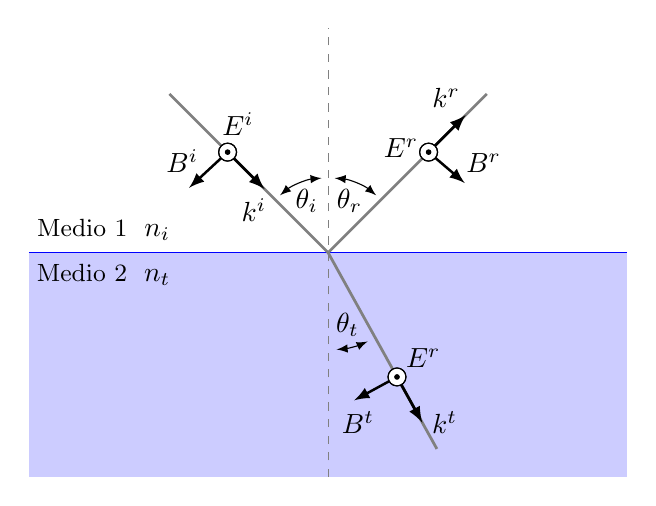
\begin{tikzpicture}[scale=.95]

%-------------------------------------------- Incidence media
\fill[blue!20] (-4,-3) rectangle (4,0);
% Interface
\draw[blue,line width=.5pt](-4,0)--(4,0); %%..5pt, interface]
% Vertical dashed line
\draw[dashed,gray,](0,-3)--(0,3);
% Media names
\node at (-3,.3) {{\small Medio 1} $\; n_i$}; 
\node at (-3,-.3) {{\small Medio 2} $\; n_t$};

%--------------------------------------------  Incident Wave
\draw[gray, line width=1pt](0:0cm)--(135:3cm);  % Light trajectory
\path (0,0)++(112.5:.75cm)node{$\theta_i$};       % Angle
\draw[latex-latex](95:1.cm)arc(95:130:1.cm);
 
    \draw[-latex,line width=1pt](135:1.9cm)--(135:1.2cm);    %Wave vector
    \path (0,0)++(141:0.9cm)node[left]{$\vb{k}^i$};     %Wave vector label
    
    \draw[-latex,line width=.9pt](135:1.9cm)--(155:2.05cm);  %B vector
    \path (0,0)++(148:2.3cm)node{$\vb{B}^i$}; 
    
    \path (0,0)++(125:2.1cm)node{$\vb{E}^i$};       % E vector
    
    \draw [fill= white](135:1.9cm)circle (0.12cm); % Vector perp. to surface
    \draw [black](135:1.9cm)circle (0.12cm);
    \filldraw[fill=black](135:1.9cm) circle(0.03cm); %%
    
%--------------------------------------------  Reflected Wave
\draw[gray,line width=1pt](0:0cm)--(45:3cm);  % Light trajectory
\path (0,0)++(67.5:.75cm)node{$\theta_r$};       % Angle
\draw[latex-latex](85:1.cm)arc(85:50:1.cm);
 
    \draw[-latex,line width=1pt](45:1.9cm)--(45:2.6cm);    %Wave vector
    \path (0,0)++(47.5:2.8cm)node[left]{$\vb{k}^r$};     %Wave vector label
    
    \draw[-latex,line width=.9pt](45:1.9cm)--(27:2.05cm);  %B vector
    \path (0,0)++(30:2.4cm)node{$\vb{B}^r$}; 
    
    \path (0,0)++(55:1.7cm)node{$\vb{E}^r$};       % E vector
    
    \draw [fill= white](45:1.9cm)circle (0.12cm); % Vector perp. to surface
    \draw [black](45:1.9cm)circle (0.12cm);
    \filldraw[fill=black](45:1.9cm) circle(0.03cm); %%

%--------------------------------------------  Transmitted Wave
\draw[gray,line width=1pt](0:0cm)--(-61:3cm);  % Light trajectory
\path (0,0)++(-75:1cm)node{$\theta_t$};       % Angle
\draw[latex-latex](-85:1.3cm)arc(-85:-66:1.3cm);
 
    \draw[-latex,line width=1pt](-61:1.9cm)--(-61:2.6cm);    %Wave vector
    \path (0,0)++(-61:2.6cm)node[right]{$\vb{k}^t$};     %Wave vector label

    \draw[-latex,line width=.9pt](-61:1.9cm)--(-80:2.005cm);  %B vector
    \path (0,0)++(-80:2.3cm)node{$\vb{B}^t$}; 
    
    \path (0,0)++(-48:1.9cm)node{$\vb{E}^r$};       % E vector
    
    \draw [fill= white](-61:1.9cm)circle (0.12cm); % Vector perp. to surface
    \draw [black](-61:1.9cm)circle (0.12cm);
    \filldraw[fill=black](-61:1.9cm) circle(0.03cm); %%     
 
\end{tikzpicture}
	\end{subfigure}
	\begin{subfigure}{.05\textwidth}\vspace{-4.5cm}\caption{}\label{sfig:Polp}	\end{subfigure}
	\begin{subfigure}{.43\textwidth}  \hspace*{-1cm}
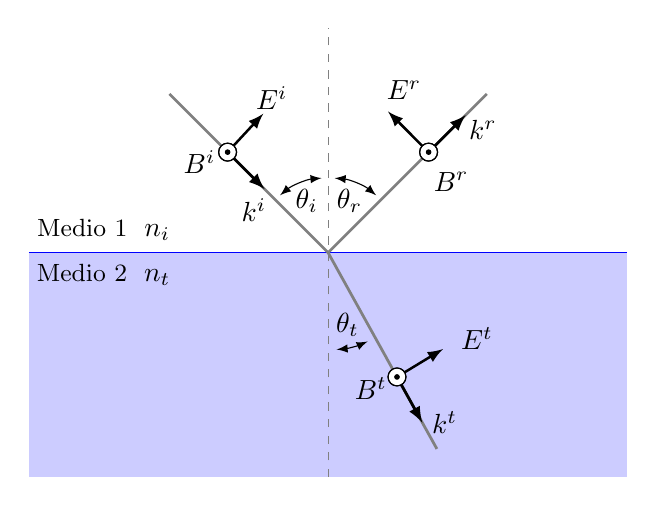
\begin{tikzpicture}[scale=.95]
%-------------------------------------------- Incidence media
\fill[blue!20] (-4,-3) rectangle (4,0);
% Interface
\draw[blue,line width=.5pt](-4,0)--(4,0); %%..5pt, interface]
% Vertical dashed line
\draw[dashed,gray,](0,-3)--(0,3);
% Media names
\node at (-3,.3) {{\small Medio 1} $\; n_i$}; 
\node at (-3,-.3) {{\small Medio 2} $\; n_t$};

%--------------------------------------------  Incident Wave
\draw[gray, line width=1pt](0:0cm)--(135:3cm);  % Light trajectory
\path (0,0)++(112.5:.75cm)node{$\theta_i$};       % Angle
\draw[latex-latex](95:1.cm)arc(95:130:1.cm);
 
    \draw[-latex,line width=1pt](135:1.9cm)--(135:1.2cm);    %Wave vector
    \path (0,0)++(141:0.9cm)node[left]{$\vb{k}^i$};     %Wave vector label
    
    \draw[-latex,line width=.9pt](135:1.9cm)--(115:2.05cm);  %E vector
    \path (0,0)++(110:2.2cm)node{$\vb{E}^i$}; 
%    \draw[-latex,line width=.9pt, red]((135:1.9cm)--(117:1.55cm); 

    
    \path (0,0)++(145:2.1cm)node{$\vb{B}^i$};       % B vector
    
    \draw [fill= white](135:1.9cm)circle (0.12cm);
    \draw [black](135:1.9cm)circle (0.12cm);
    \filldraw[fill=black](135:1.9cm) circle(0.03cm); %%    
    
    
%    \draw[line width=.6pt] (135:1.9cm)   % Esto esra paea hacer el vector salir de la hoja
%                         +(-135:.12cm) -- +(45:.12cm)
%                         +(-45:.12cm) -- +(135:.12cm);    
   
    
%--------------------------------------------  Reflected Wave
\draw[gray,line width=1pt](0:0cm)--(45:3cm);  % Light trajectory
\path (0,0)++(67.5:.75cm)node{$\theta_r$};       % Angle
\draw[latex-latex](85:1.cm)arc(85:50:1.cm);
 
    \draw[-latex,line width=1pt](45:1.9cm)--(45:2.6cm);    %Wave vector
    \path (0,0)++(43:2.4cm)node[right]{$\vb{k}^r$};     %Wave vector label
    
    \draw[-latex,line width=.9pt](45:1.9cm)--(67:2.05cm);  %E vector
    \path (0,0)++(65:2.4cm)node{$\vb{E}^r$};
  %  \draw[-latex,line width=.9pt, red](45:1.9cm)--(59:1.55cm); 
   % \draw[dashed,red,line width=.9pt](59:1.55cm)--(67:2.05cm);
    
    \path (0,0)++(30:1.9cm)node{$\vb{B}^r$};       % B vector
    
    \draw [fill= white](45:1.9cm)circle (0.12cm);
    \draw [black](45:1.9cm)circle (0.12cm);
    \filldraw[fill=black](45:1.9cm) circle(0.03cm); %%  


%--------------------------------------------  Transmitted Wave
\draw[gray,line width=1pt](0:0cm)--(-61:3cm);  % Light trajectory
\path (0,0)++(-75:1cm)node{$\theta_t$};       % Angle
\draw[latex-latex](-85:1.3cm)arc(-85:-66:1.3cm);
 
    \draw[-latex,line width=1pt](-61:1.9cm)--(-61:2.6cm);    %Wave vector
    \path (0,0)++(-61:2.6cm)node[right]{$\vb{k}^t$};     %Wave vector label
 
    \draw[-latex,line width=.9pt](-61:1.9cm)--(-40:2.005cm);  %E vector
%      \draw[-latex,line width=.9pt, red](-61:1.9cm)--(-45:2.3cm); 
    \path (0,0)++(-30:2.3cm)node{$\vb{E}^t$}; 
    
    \path (0,0)++(-72.5:1.9cm)node{$\vb{B}^t$};       % B vector
    
    \draw [fill= white](-61:1.9cm)circle (0.12cm);
    \draw [black](-61:1.9cm)circle (0.12cm);
    \filldraw[fill=black](-61:1.9cm) circle(0.03cm); %% 
\end{tikzpicture}
	\end{subfigure} 
	\caption{ Esquema de de una onda plana en polarización \textbf{a)} \emph{s} y \textbf{b)} \emph{p} que se propaga en una dirección $\vb{k}^i$ e incide con un ángulo de incidencia $\theta_i$ en una interfaz plana entre dos medio lineales, homogéneos e isótropos, donde el medio de incidencia tiene un índice de refracción $n_i$ y el de transmisión, $n_t$. El haz reflejado se propaga con un ángulo $\theta_r=\theta_i$ según la ley de reflexión [Ec. \eqref{eq:LeyReflexion}] y el ángulo transmitido se propaga con un ángulo $\theta_t$ dado por la ley de Snell [Ec. \eqref{eq:LeySnell}]. En el esquema se asume que la orientación de los campos EMs incidentes  ($\vb{E}^i,\,\vb{B}^i$) es la misma para los campos EMs reflejados ($\vb{E}^r,\,\vb{B}^r$) y transmitidos ($\vb{E}^t,\,\vb{B}^t$).}	\label{fig:Polarizaciones}	
	\end{figure}	
%

Para polarización \emph{s} y medios no magnéticos ($\mu=\mu_0$),  el campo eléctrico es perpendicular al plano de incidencia y paralelo a la interfaz por lo que, mediante la Ec. \eqref{seq:Epara}, $E^i + E^r = E^t$, en donde se asume que la orientación del campo eléctrico incidente se preserva tras la reflexión y la transmisión, como se observa en la Fig. \ref{sfig:Pols}. Al emplear la continuidad de la componente paralela a la interfaz de $\vb{B}/\mu$ [Ec. \eqref{seq:Bpara}], la relación $E = (c/n) B$ y la ley de la reflexión [Ec. \eqref{eq:LeyReflexion}] y de Snell [Ec. \eqref{eq:LeySnell}] se obtienen los coeficientes de amplitud $r$ y $t$ para  polarización \emph{s}, dados por\vspace{-.5em}\index{Fresnel!amplitud, coeficientes de ($r,t$)!$s$}
%
	\begin{tcolorbox}[title = Coeficientes de amplitud para polarización \emph{s} ]
	\vspace*{-1em}	
	\eqhalf{r_s =
		\frac{n_i\cos\theta_i-\sqrt{n_t^2-n_i^2\sin ^2\theta_i}}
 			{n_i \cos\theta_i + \sqrt{ n_t^2-n_i^2\sin ^2\theta_i}}, 
 			\label{eq:rs}}
	\eqhalf{ t_s =
		\frac{2n_i\cos\theta_i}
 			{n_i\cos\theta_i + \sqrt{ n_t^2-n_i^2\sin ^2\theta_i}}.
 			\label{eq:ts}}
	\end{tcolorbox}	 \vspace*{-.75em}\noindent
%
Cuando el campo eléctrico es paralelo al plano de incidencia, y por tanto perpendicular a la interfaz como se observa en la Fig. \ref{sfig:Polp}, se cumple la relación $E^i\cos\theta_i-E^r\cos\theta_r = E^t \cos\theta_t$ por la Ec. \eqref{seq:Epara}. Al asumir nuevamente que la orientación de oscilación del campo eléctrico reflejado y transmitido coincide con la del campo eléctrico incidente, y al emplear las Ecs. \eqref{seq:Bpara},  \eqref{eq:LeyReflexion} y  \eqref{eq:LeySnell}, así como la relación $E = (c/n) B$, se calculan los  coeficientes de amplitud $r$ y $t$ para  polarización \emph{p}, dados por \index{Fresnel!amplitud, coeficientes de ($r,t$)!$p$} \vspace*{-.75em}
	\begin{tcolorbox}[title = Coeficientes de amplitud para polarización \emph{p} ]
	\vspace*{-1em}
	\eqhalf{ r_p =
				\frac{n_t^2\cos\theta_i -n_i\sqrt{n_t^2-n_i^2\sin^2\theta_i}}
 				{n_t^2\cos\theta_i +n_i\sqrt{n_t^2-n_i^2\sin^2\theta_i}}, \label{eq:rp}}
	\eqhalf{ t_p =
				\frac{ 2 n_i n_t \cos\theta_i}
 				{n_t^2\cos \theta_i+n_i\sqrt{n_t^2-n_i^2\sin^2\theta_i}}.
 				\label{eq:tp}}
	\end{tcolorbox}	

Dado que los coeficientes  de amplitud dependen de los índices de refracción de los medios que conforman la interfaz, es posible hacer la distinción entre dos casos al analizar el término dentro de la raíz cuadrada en las Ecs. \eqref{eq:rs}--\eqref{eq:tp}: incidencia externa ($n_t>n_i$) e incidencia interna ($n_t<n_i$). En la Fig. \ref{fig:coefAmp} se grafican los coeficientes de amplitud $r$ (líneas continuas) y $t$ (líneas discontinuas) como función del ángulo de incidencia $\theta_i$ para una interfaz de entre aire ($n= 1$) y un medio con un índice de refracción $n = 1.5$, en configuración de incidencia externa [Fig. \ref{sfig:coefExt}] e interna [Fig. \ref{sfig:coefInt}] para ambas polarizaciones, en donde las líneas azules corresponden a la polarización \emph{s} y las rojas a \emph{p}. Dado que se cumple para amos medios que $n = \sqrt{\varepsilon}>0$, ninguno de los dos medios es absorbente. \index{Incidencia!interna}\index{Incidencia!externa}
%
\begin{figure}[h!]\centering\hspace*{-1.5em}
	\begin{subfigure}{.05\textwidth}\vspace{-4.5cm}\caption{}\label{sfig:coefExt}\end{subfigure}
	\begin{subfigure}{.43\textwidth} \hspace*{-.8cm}
	\includegraphics[scale=1]{1-Teoria/figs/1-1-ampCoefExt}
	\end{subfigure}
	\begin{subfigure}{.05\textwidth}\vspace{-4.5cm}\caption{}\label{sfig:coefInt}\end{subfigure}
	\begin{subfigure}{.43\textwidth} \hspace*{-.9cm}
	\includegraphics[scale=1]{1-Teoria/figs/1-1-ampCoefInt}
	\end{subfigure}\vspace*{-.7em}
	\caption{ Coeficientes de amplitud $r$ (líneas continuas) y $t$ (líneas discontinuas), como función del ángulo de incidencia $\theta_i$, en configuración de incidencia \textbf{a)} externa e \textbf{b)} interna para una interfaz entre  aire ($n=1$) y un medio con índice de refracción $n = 1.5$. Los cálculos para polarización  \emph{s} se muestran  en azul y  para \emph{p} en rojo. }	\label{fig:coefAmp}	
	\end{figure}	

En la Fig. \ref{fig:coefAmp} el coeficiente de amplitud de reflexión $r_p$ [Ec. \eqref{eq:rp}] toma un valor nulo para el ángulo de incidencia  denominado ángulo de Brewster $\theta_B$, que cumple con la expresión\index{Ángulo!de Brewster} \index{Brewster!ángulo de}
%
	\begin{align}
	\tan\theta_B = \frac{n_t}{n_i},
	\label{eq:Brewster}
	\end{align}
%	
tanto para incidencia externa [Fig. \ref{sfig:coefExt}], donde $\theta_B \approx 56^\circ$, como para interna [Fig. \ref{sfig:coefInt}], donde $\theta_B \approx 33^\circ$. El cambio de signo del coeficiente de reflexión $r_p$ para $\theta_i>\theta_B$ corresponde a un cambio de fase de $\pi$ radianes del campo eléctrico reflejado respecto al campo eléctrico incidente. De la Ec. \eqref{eq:Brewster} se deduce que el ángulo de Brewster de incidencia externa $\theta_B^{ext}$ es complementario al de incidencia interna $\theta_B^{int}$, es decir, $\theta_B^{ext}+\theta_B^{int} = 90^\circ$ como se observa en las gráficas de la Fig. \ref{fig:coefAmp}. Cuando se considera una configuración de incidencia interna, se cumple la relación $n_i>n_t$, por lo que los coeficientes de amplitud  [Ecs. \eqref{eq:rs}--\eqref{eq:tp}] son cantidades complejas para un ángulos de incidencia mayores al ángulo crítico $\theta_c$ que cumple la expresión\index{Ángulo!crítico|see {Incidencia interna}}\index{Ángulo!crítico}
% 
	\begin{align}
	\sin\theta_c = \frac{n_t}{n_i}.
	\label{eq:Criticp}
	\end{align}
%
Al sustituir la Ec. \eqref{eq:Criticp} en la ley de Snell [Ec. \eqref{eq:LeySnell}] se obtiene que $\theta_t = 90^\circ$ por lo que para $\theta_i>\theta_c$ toda la luz es reflejada y no transmitida, es decir, se está en el régimen \emph{reflexión total interna} \index{Reflexión total!interna}. En la Fig. \ref{sfig:coefInt} se observa que los coeficientes de amplitud son máximos en $\theta_c \approx 48^\circ$ sin embargo, para $\theta_i>\theta_c$, los coeficientes de amplitud  [Ecs. \eqref{eq:rs}--\eqref{eq:tp}] son cantidades complejas, lo que indica que los campos eléctricos reflejado y transmitido tienen un desfase, distinto de $\pi$ radianes, respecto al campo eléctrico incidente.  Para corroborar que toda la luz es reflejada en incidencia interna para $\theta_i>\theta_c$ se considera la conservación de la energía transportada por los campos EMs al cruzar la interfaz.

El análisis del comportamiento de las ondas EMs al cruzar una interfaz plana, entre dos medios lineales homogéneos e isótropos, en términos de las amplitudes de los campos eléctricos describen el comportamiento de la magnitud y los cambios de fase en los campos eléctricos y no la energía transportada por los campos EMs reflejados y transmitidos. Al emplear vector de Poynting [Ec. (\ref{eq:Poynting})] y calcular su promedio temporal\footnote{El promedio temporal del vector de Poynting es $\langle\vb{S}\rangle_t = (1/\tau)\int_t^{t+\tau}\vb{S}(t')dt'$, y para campos EMs tipo ondas planas es $\langle\vb{S}\rangle_t = (1/2) \Re[\vb{E}\times\qty(\vb{B}/\mu)^*]$.\index{Poynting!vector de!promedio temporal del}} se calcula la irradiancia $I$ \cite{hecht1998optics}, dada por
	\begin{align}
	I = \langle S \rangle_t = \frac{nc\varepsilon_0}{2} EE^*,
	\label{eq:Irr}
	\end{align}
que corresponde a la energía promedio por unidad de tiempo y unidad de área, transportada por los campos EMs en la dirección $\vu{k}$ \cite{griffiths2013electrodynamics}. Para calcular la energía por unidad de tiempo $P$ transportada por los campos EMs al cruzar la interfaz se multiplica la Ec. \eqref{eq:Irr} por la sección transversal de un haz de luz. En la Fig. \ref{fig:hazcircular} se muestran las secciones transversales de un haz  que incide a un ángulo $\theta_i$ sobre la interfaz entre dos medios con índice de refracción $n_i$ y $n_t$, respectivamente. Cuando el haz se refleja, a un ángulo $\theta_r=\theta_i$, y se refracta a un ángulo $\theta_t$, la sección transversal del haz cambia. Si el área de los haces justo en la interfaz es $A$, mediante la ley de la reflexión [Ec. \eqref{eq:LeyReflexion}] y la ley de Snell [Ec. \eqref{eq:LeySnell}], la sección transversal del has incidente y el reflejado  es $A\cos\theta_i$, mientras que la del haz transmitido es $A\cos\theta_t$.

	\begin{figure}[h]\centering
\begin{tikzpicture}[scale=.7]
%\draw (3.46,1.9) circle(2pt);ESTA ES LAREFERENCIA PARA ANTES DE MOVER LAS COSAS

%---------------------------------------------------------------------------------------- SUPERFICIE
\fill[blue!20]			
(-5,-1) -- (-3,2) 
-- (3,2) -- (5,-1)
--(-5,-1);						

\draw[dashed,gray](0,-4)--(0,5);  %---------------------------------------------------- Vertical dashed line

\node at (-4,-.5) {Medio 1 $\; n_i$}; %-------------------------------------------------- media names
\node at (-4,-1.5) {Medio 2 $\; n_t$};

%---------------------------------------------------------------------------------------- SPOT INTERFAZ
\fill[lgreen, opacity= .75] (0,.5) circle (2 and .6); 
\draw[black](0,.5) circle (2 and .6)		% -------------------------------------------  Etiqueta área
			(0,.5)node[]{$A$};	
%------------------------------------------------------------- INCIDENTE
\path[shift = {(0,1.7)}] (0,0)++(112.5:1cm)node{$\theta_i$};   %---------- Angle
\draw[latex - latex,shift = {(0,2.1)}](-1,.5)arc(144.5:90:1.1cm);

\draw [-,shift = {(-2,.5)}, rotate = 55.5] (0,0) -- (0,3.2);%Cara del cilindro(Rota desde 90°)
\draw[-, shift = {(2,.5)},rotate = 55.5] (0,0) -- (0,6.3);

\draw[black, rotate = 50.75, shift = {(0,5)}](0,0) circle (1.145 and .3);% Tapa del cilidndro del del área
\node at (-5.1,3.5) { $A\cos\theta_i$};
\fill[lgreen, opacity= .5, rotate = 50.75, shift = {(0,5)}](0,0) circle (1.145 and .3);

%-------------------------------------------------------------- REFLEJADO
\path[shift = {(0,1.7)}] (0,0)++(67.5:1cm)node{$\theta_r$};   %------------- Angle
\draw[latex - latex ,shift = {(0,2.1)}](1,.5)arc(35:90:1.1cm);

\draw [-,shift = {(-2,.5)}, rotate = -55.5] (0,0) -- (0,6.3);  %- Cara del cilindro
\draw[-, shift = {(2,.5)},rotate = -55.5] (0,0) -- (0,3.2);

\draw[black, rotate = -50.75, shift = {(0,5)}](0,0) circle (1.145 and .3); %Tapa del cilidndro del del área
\node at (5.1,3.5) { $A\cos\theta_r$};
\fill[lgreen , opacity= .5, rotate = -50.75, shift = {(0,5)}](0,0) circle (1.145 and .3);

%----------------------------------------------------------------- TRANSMITIDO
\path  (0,0)++(275:4.1)node{$\theta_t$};    %------------------------- Angle
\draw[latex - latex](0,-3.5)arc(270:290:1.5cm);

\draw [-,shift = {(-2,.5)}, rotate = 33.5] (0,0) -- (0,-5);   %------------------------- Cara del cilindro
\draw[-, shift = {(2,.5)},rotate = 33.5] (0,0) -- (0,-3.1);

\draw[black, rotate = 29.2, shift = {(.5,-3.6)}](0,0) circle (1.675 and .3);		%-------- Tapa del cilidndro del del área
\node at (3.5,-3.5) {$A\cos\theta_t$};
\fill[lgreen, opacity= .5,  rotate = 29.2, shift = {(.5,-3.6)}](0,0) circle (1.675 and .3);

\end{tikzpicture}
	\caption{Sección transversal de un haz de luz incidiendo en una interfaz entre dos medio lineales, homogéneos e isótropos con índices de refracción $n_i$ y $n_t$. El haz incide sobre la interfaz a un ángulo de $\theta_i$, se refleja con un ángulo $\theta_r$ y se transmite a un ángulo $\theta_t$, calculados medinate las ley de la reflexión y de Snell, respectivamente. El área del haz sobre la interfaz es $A$, mientras que en los haces, al propagarse, es $A\cos\theta$, en donde $\theta$ es el ángulo de propagación respectivo para cada haz.} \label{fig:hazcircular}
	\end{figure}

 Al emplear la Ec. \eqref{eq:Irr} y multiplicarla por el área de alguno de los tres haces mostrados en la Fig. \ref{fig:hazcircular}, se obtiene que la energía por unidad de tiempo transportada por cada haz de luz es
	\begin{align*}
	P = I A \cos\theta = \frac{n c \varepsilon_0}{2}  EE^* \cos\theta,
	\end{align*}
en donde el ángulo $\theta$ e indice de refracción $n$ toman los valores de $\theta_i$ y $n_i$ para el haz incidente y el reflejado, mientras que  toma los valores de $\theta_t$ y  $n_t$ para el haz transmitido. Cuando se normaliza la energía por unidad de tiempo transportada por el haz reflejado y por el haz transmitido, entre la del haz incidente se obtienen las expresiones de la reflectancia $R$ y la transmitancia $T$ \vspace{-.5em} \index{Fresnel!Reflectancia ($R$)}\index{Fresnel!Transmitancia ($T$)}
	\begin{tcolorbox}[title = Reflectancia y transmitancia]
	\eqhalf{ R =  r r^*, \label{eq:R}}
	\eqhalf{ T = \frac{n_t\cos\theta_i}{n_i \cos\theta_t} t t^*,\label{eq:T}}
	\end{tcolorbox}\vspace*{-.75em}\noindent	
en donde $r$ es el coeficiente de amplitud de reflexión y $t$ el de transmisión, dados por las Ecs. \eqref{eq:rs}--\eqref{eq:tp}.

En la Fig. \ref{fig:frsnel} se presentan la reflectancia (líneas continuas) y transmitancia (líneas discontinuas) como función del ángulo de incidencia $\theta_i$, para la polarización \emph{s} (en azul) y \emph{p} (en rojo), de un haz de luz que incide en la interfaz entre aire ($n=1$) y un medio con índice de refracción $n=1.5$ para una configuración de incidencia externa [Fig. \ref{sfig:frsnelExt}] e incidencia interna [Fig. \ref{sfig:frsnelExt}].
%
\begin{figure}[h!]\centering\hspace*{-1.5em}
	\begin{subfigure}{.05\textwidth}\vspace{-4.5cm}\caption{}\label{sfig:frsnelExt}\end{subfigure}
	\begin{subfigure}{.43\textwidth} \hspace*{-.7cm}
	\includegraphics[scale=1]{1-Teoria/figs/1-2-FrsnelExt}
	\end{subfigure}
	\begin{subfigure}{.05\textwidth}\vspace{-4.5cm}\caption{}\label{sfig:frsenlInt}\end{subfigure}
	\begin{subfigure}{.43\textwidth} \hspace*{-.7cm}
	\includegraphics[scale=1]{1-Teoria/figs/1-2-FrsnelInt}
	\end{subfigure}\vspace*{-.7em}
	\caption{  Reflectrancia (líneas continuas) y transmitancia (líneas discontinuas), como función del ángulo de incidencia $\theta_i$, en configuración de incidencia \textbf{a)} externa e \textbf{b)} interna para una interfaz entre  aire ($n=1$) y un medio con índice de refracción $n = 1.5$. Los cálculos para polarización  \emph{s} se muestran  en azul y  para \emph{p} en rojo.}	\label{fig:frsnel}	
	\end{figure}	
%

El ángulo de Brewster $\theta_B$ es apreciable en las gráficas de la Fig. \ref{fig:frsnel}, en donde se observa $R_p = 0$. Asimismo es apreciable en la Fig. \ref{sfig:frsenlInt} que para ángulos de incidencia mayores al ángulo crítico, se cumple que $R_p = R_s = 1$, mientras que $T_s = T_p = 0$, es decir, que toda la luz es reflejada. En la Fig. \ref{fig:frsnel} se observa que es válida la relación $R + T = 1$ sin embargo, ésta es válida únicamente para índices de refracción $n = \sqrt{\varepsilon}$ que sean cantidades reales, dado que para medios no magnéticos ($\mu_0 = \mu$), la parte imaginaria de la función dieléctrica $\Im[\varepsilon]$ se asocia con la absorción de energía por el material \cite{ibach2003solid}. Cuando la luz se propaga a través de algún medio absorbente, se cumple en general 
	\begin{align*}
	R + T + A = 1,
	\end{align*}
en donde el término $A$ es la energía absorbida por el material, relativa a la energía del haz incidente.\index{Función dieléctrica!Absorción}
	
\section{Solución de Mie}

\index{Mie!solución de}\index{Esparcimiento! de luz|see{Mie}}
El problema de absorción y esparcimiento de luz por una partícula esférica fue resuelto por el físico alemán Gustav Mie en 1908 \cite{mie1908metallosung}. La solución de Mie consiste en expandir una onda plana, que ilumina a una esfera de tamaño y material arbitrario, en una base de armónicos esféricos vectoriales que son una base ortogonal esférica y cuyos elementos satisfacen las ecuaciones de Maxwell \cite{bohren1998absorption}. Al considerar las condiciones de contorno que satisfacen los campos EMs sobre la superficie de la esfera, se escriben los campos EMs dentro de la partícula y los campos esparcidos por ésta como una serie en la base de los armónicos esféricos vectoriales, cuyos coeficientes corresponden a una expanción multipolar y son conocidos como los coeficientes de Mie \cite{bohren1998absorption}. A pesar de que existen publicaciones previas a la de Mie en donde  el problema de la absorción y esparcimiento de luz es tratado de forma semejante, el trabajo de Mie destacó debido al desarrollo de relaciones recursivas que facilitan el cálculo numérico y se discute la convergencia de este resultado \cite{horvath2009historic}. El desarrollo de una solución apta para el cálculo numérico permitió que en el artículo de Mie se describieran diez propiedades de la luz al interactuar con suspenciones diluidas de partículas esféricas \cite{mie1908metallosung}, lo que contribuyó al impacto de su solución sobre el trabajo de otros autores \cite{horvath2009historic}. 

	\begin{figure}[b!]\centering
	\tdplotsetmaincoords{60}{110}
	\pgfmathsetmacro{\rvec}{1. 3}
	\pgfmathsetmacro{\thetavec}{30}
	\pgfmathsetmacro{\varphivec}{60}
\begin{tikzpicture}[scale=3.5,tdplot_main_coords]
%draw the NP
	\draw[tdplot_screen_coords,ball color=yellow, opacity = 1] (0,0,0) circle (.05);
	\draw[tdplot_screen_coords, color=yellow, opacity = 1] (0,0,0) circle (.05);


%set up some coordinates 
	\coordinate (O) at (0,0,0);

%determine a coordinate (P) using (r,\theta,\varphi) coordinates.   This command
%also determines (Pxy), (Pxz), and (Pyz): the xy-, xz-, and yz-projections
%of the point (P). 
%syntax: \tdplotsetcoord{Coordinate name without parentheses}{r}{\theta}{\varphi}
	\tdplotsetcoord{P}{\rvec}{\thetavec}{\varphivec}

%draw figure contents
%--------------------
%draw the main coordinate system axes
	\draw[thick,- latex] (0,0,0) -- (1. 5,0,0) node[anchor=north east]{$x$};
	\draw[thick,- latex] (0,0,0) -- (0,1. 5,0) node[anchor=north west]{$y$};
	\draw[thick,- latex] (0,0,0) -- (0,0,1. 5) node[anchor=south]{$z$};

%draw the main cartesian vector system 
	\draw[thick,- latex, blue] (0,0,0) -- (1,0,0) node[anchor= south east]{$\vu{e}_x$};
	\draw[thick,- latex, blue] (0,0,0) -- (0,1,0) node[anchor=north west]{$\vu{e}_y$};
	\draw[thick,- latex, blue] (0,0,0) -- (0,0,1) node[anchor= east]{$\vu{e}_z$};

%draw a vector from origin to point (P) 
	\draw[thick,color=green, - latex] (O) -- (P);
	\node at (1,. 5,1. 1) {\color{green} $\vb{r}$};

%draw projection on xy plane, and a connecting line
	\draw[dashed, color=green] (O) -- (Pxy);
	\draw[dashed, color=green] (P) -- (Pxy);
	\fill[green, opacity = . 3] (O) --(Pxy)-- (P)--(O);
	\draw[- latex, tdplot_screen_coords,green](.42,.2)--(.8,.2);
	\node[tdplot_screen_coords] at (1.35,.2) {\color{green}\small Plano de esparcimiento};


%draw the angle \varphi, and label it
	%syntax: \tdplotdrawarc[coordinate frame, draw options]{center point}{r}{angle}{label options}{label}
	\tdplotdrawarc[- latex]{(O)}{0. 5}{0}{\varphivec}{anchor=south}{$\varphi$}


%set the rotated coordinate system so the x'-y' plane lies within the
	%"theta plane" of the main coordinate system
	%syntax: \tdplotsetthetaplanecoords{\varphi}
	\tdplotsetthetaplanecoords{\varphivec}

%draw theta arc and label, using rotated coordinate system
	\tdplotdrawarc[tdplot_rotated_coords, - latex]{(0,0,0)}{0. 45}{0}{\thetavec}{anchor=north}{$\theta$}

%draw some dashed arcs, demonstrating direct arc drawing
	\draw[dashed,tdplot_rotated_coords] (\rvec,0,0) arc (0:90:\rvec);
	\draw[dashed] (\rvec,0,0) arc (0:90:\rvec);

%set the rotated coordinate definition within display using a translation
%coordinate and Euler angles in the "z(\alpha)y(\beta)z(\gamma)" euler rotation convention
%syntax: \tdplotsetrotatedcoords{\alpha}{\beta}{\gamma}
	\tdplotsetrotatedcoords{\varphivec}{\thetavec}{0}

%translate the rotated coordinate system
%syntax: \tdplotsetrotatedcoordsorigin{point}
	\tdplotsetrotatedcoordsorigin{(P)}

%use the tdplot_rotated_coords style to work in the rotated, translated coordinate frame
	\draw[thick,tdplot_rotated_coords,- latex, purple] (0,0,0) -- (. 3,0,0) node[anchor=north west]{{\color{black}$\vu{e}_\theta,$}$\vu{e}_{\parallel}^s$};
	\draw[thick,tdplot_rotated_coords,- latex,black] (0,0,0) -- (0,. 3,0) node[anchor=west]{$\vu{e}_\varphi$};
	\draw[thick,tdplot_rotated_coords,- latex,purple] (0,0,0) -- (0,-. 3,0) node[anchor= north west]{$\vu{e}_{\perp}^s$};
	\draw[thick,tdplot_rotated_coords,- latex] (0,0,0) -- (0,0,. 3) node[anchor=south]{$\vu{e}_r$ };



%set the rotated coordinate definition within display using a translation
%coordinate and Euler angles in the "z(\alpha)y(\beta)z(\gamma)" euler rotation convention
%syntax: \tdplotsetrotatedcoords{\alpha}{\beta}{\gamma}
	\tdplotsetrotatedcoords{\varphivec}{0}{0}

%translate the rotated coordinate system
%syntax: \tdplotsetrotatedcoordsorigin{point}
	\tdplotsetrotatedcoordsorigin{(Pxy)}

	\draw[thick,tdplot_rotated_coords,- latex, purple] (0,0,0) -- (. 3,0,0) node[anchor= west]{$\vu{e}_{\parallel}^i$};
	\draw[thick,tdplot_rotated_coords,- latex, blue] (0,0,0) -- (0,0,. 3) node[anchor= west]{$\vu{e}_z$};	
	\draw[thick,tdplot_rotated_coords,- latex, purple] (0,0,0) -- (0,-. 3,0) node[anchor= north west]{$\vu{e}_{\perp}^i$};



% Plane Wave
	\foreach \i in {-7,...,-2}{
		\draw[thick,tdplot_screen_coords,red, - latex] (\i/10,0,0)--(\i/10,1,0);}
	\node[tdplot_screen_coords] at (-4.5/10,1.1,0){\color{red}$\vb{k}_i$};
	\node[tdplot_screen_coords] at (-4.5/10,-.1,0){\small \color{red}Haz incidente};
\end{tikzpicture}
%
\caption{Diagrama del plano de esparcimiento (en verde) definido por el vector $\vb{r}$, posición donde se evalúan los campos EMs, y el vector $\vu{e}_z$, cuando una onda plana propagándose en dirección $z$ (en rojo) ilumina a una partícula arbitraria.  La base canónica cartesiana para vectores se muestra en azul, mientras que la base canónica esférica se muestra en negro.  Las direcciones paralelas $\parallel$ y perpendiculares $\perp$ al plano de incidencia  para el campo eléctro incidente, denotado por el subíndice $i$ y el esparcido, denotado por el subíndice $s$ se muestran en morado.  En ambas figuras, el haz incidente se muestra en rojo.}\label{fig:PlanoEsparcimiento}
	\end{figure}	

Para el estudio del esparcimiento por una partícula arbitraria inmersa en un medio con índice de refracción $n_m$, denominado  matriz, se considera que la partícula es iluminada por una onda plana con una longitud de onda $\lambda$, cuya dirección de propagación define la dirección $z$, es decir,
	\begin{align}
	\vb{E}^i = (E_x^i \vu{e}_x + E_y^i \vu{e}_y)e^{i(k z - \omega t)},
	\label{eq:Exyi}
	\end{align}
donde $k = 2\pi n_m /\lambda$ es el número de onda. En la Fig.  \ref{fig:PlanoEsparcimiento} se muestra  una partícula localizada en el origen iluminada por una onda plana [Ec. \eqref{eq:Exyi}] que se propaga en la dirección $z$.  De forma análoga al plano de incidencia, se define el plano de esparcimiento (en verde en la Fig. \ref{fig:PlanoEsparcimiento}) con el vector de dirección del esparcimiento $\vu{e}_r$ y la dirección del haz incidente $\vu{e}_z$. Con base en el plano de esparcimiento es posible definir las componentes ortogonales $\perp$ y paralelas $\parallel$ de los campos EMs, así como su polarización. \index{Plano!de esparcimiento} \index{Polarización!respecto al plano de esparcimiento}

Como se muestra en la Fig. \ref{fig:PlanoEsparcimiento}, los vectores unitarios perpendicular y paralelo al plano de esparcimiento de la onda incidente, $\vu{e}_{\perp}^i$  y $\vu{e}_{\parallel}^i$, respectivamente, y de los campos EMs esparcidos $\vu{e}_{\perp}^s$ y $\vu{e}_{\parallel}^s$ están dados por%
\begin{subequations} \index{Polarización!respecto al plano de esparcimiento!paralela ($\parallel$)}\index{Polarización!respecto al plano de esparcimiento!perpendicular ($\perp$)}\vspace*{-2em}

	\eqhalf{\vu{e}_{\perp}^i =-\, \hat{e}_\varphi  = \sin\varphi\,\vu{e}_x - \cos\varphi\,\vu{e}_y,}	
	\eqhalf{\vu{e}_{\parallel}^i = \cos\varphi\,\vu{e}_x + \sin\varphi\,\vu{e}_y,}	
	\label{eqs:vecInc}\end{subequations}	\begin{subequations}
	\eqhalf{\vu{e}_{\perp}^s= - \, \vu{e}_\varphi,}	
	\eqhalf{\vu{e}_{\parallel}^s = \vu{e}_\theta.}	
	\label{eqs:vecScat}\end{subequations}\vspace*{-1em}
	
Al despejar $\vu{e}_x$ y $\vu{e}_y$  de las Ecs. \eqref{eqs:vecInc}, y reescribirlos en la base de los vectores unitarios en la dirección perpendicular y normal al plano de esparcimiento como $\vu{e}_x = \sin\varphi\,\vu{e}_{\perp}^i + \cos\varphi\,\vu{e}_{\parallel}^i, $ y $\vu{e}_y = - \cos\varphi \,\vu{e}_{\perp}^i + \sin\varphi\,\vu{e}_{\parallel}^i$ se obtiene que $\vb{E}^i$ [Ec. \eqref{eq:Exyi}] se puede escribir como
\begin{align}
\vb{E}^i = [(\cos\varphi E_{x}^i + \sin\varphi E_{y}^i)\vu{e}_{\perp}^i +
			 (\sin\varphi E_{x}^i - \cos\varphi E_{y}^i)\vu{e}_{\parallel}^i]
			 e^{ikz}
			 = E_{\perp}^i  \vu{e}_{\perp}^i + E_{\parallel}^i\vu{e}_{\parallel}^i
		\label{eq:EIncidente}
\end{align}
en donde se omite el término de la fase temporal $e^{-i\omega t}$ y la fase espacial $e^{ikz}$ se incluye en los coficientes $E_\perp^i$ y $E_\parallel^i$. Adicionalmente, al considerar para el campo eléctrico esparcido  únicamente los términos que corresponden al campo lejano, es decir, el término con componentes transversales y que decae como $r^{-1}$ y cumple con la relación $kr\ll 1$, el campo esparcido $\vb{E}^s$ puede escribirse como \cite{bohren1998absorption}\index{Electromagnéticos!campos!lejano}
	\begin{align}
	\vb{E}^s \propto \frac{e^{ikr}}{-ikr}\vb{E}_0^s 
			=  \frac{e^{ikr}}{-ikr}
			\qty( E_{\perp}^s  \vu{e}_{\perp}^s + E_{\parallel}^s \vu{e}_{\parallel}^s) \label{eq:ELejano}
	\end{align}
en donde  $\vb{E}_0^s$ es la amplitud del campo esparcido,  $ E_{\perp}^s$ y  $ E_{\parallel}^s$ sus componentes en la base de los vectores paralelo y perpendicular al plano de esparcimiento [Ec. \eqref{eqs:vecScat}]. Asimismo, es posible relacionar al campo eléctrico esparcido por una partícula localizada en el centro de coordenadas $\vb{E}^s$ [Ec. \eqref{eq:ELejano}] con el  campo eléctrico incidente $\vb{E}^i$ [Ec. \eqref{eq:EIncidente}]  mediante  la diadica de esparcimiento de campo lejano  $\mathbb{F}(\vu{k}^i,\vu{k}^s)$ \index{Electromagnéticos!campos!diadica de campo lejano} \cite{tsang2000scattering}
	\begin{align}
	\vb{E}^s = \frac{e^{i\vb{k}^s\cdot\vb{r}}}{r}\mathbb{F}(\vu{k}^i,\vu{k}^s)\vb{E}^i
	\label{eq:FarFieldDyadic}
	\end{align}
donde $\mathbb{F}$ depende de de la dirección de la onda plana incidente $\vu{k}^i$ y la dirección del campo eléctrico esparcido $\vu{k}^s$. Al considerar la forma asintótica del campo eléctrico esparcido [Ec. \eqref{eq:ELejano}] y su relación con el campo eléctrico incidente [Ec. \eqref{eq:FarFieldDyadic}], se pueden relacionar las componentes perpendiculares del campo esparcido y el campo incidente de una onda plana en la base de los vectores perpendiculares y paralelos al plano de incidencia mediante la matriz de esparcimiento $\mathbb{S}$ \index{Esparcimiento!matriz de} \cite{bohren1998absorption}
	\begin{align}
	\mqty(E_{\parallel}^s\\E_{\perp}^s) = 
		\frac{e^{ik(r-z)}}{-ikr} \mqty(S_2&S_3\\S_4&S_1)
	\mqty(E_{\parallel}^i\\E_{\perp}^i),\label{eq:MEsparcimientoGral}
	\end{align}
en donde, de forma general, $S_j = S_j(\theta,\varphi)$, con $j=1,2,3$ y $4$, además de que las componentes de la matriz de esparcimiento en la Ec. \eqref{eq:MEsparcimientoGral} dependen de la geometría de la partícula iluminada por la onda plana.

	\subsection{Solución a la ecuación de onda con simetría esférica}


Las ecuaciones de Maxwell, al considerar una región del espacio sin fuentes externas, y campos EMs armónicos en el tiempo, se reescriben como \cite{jackson1999electrodynamics} \index{Maxwell!ecuaciones de!transformada de Fourier de las}

	\begin{subequations}
	\eqhalf{\nabla\cdot \vb{E} = 0, }
	\eqhalf{\nabla\cdot \vb{H} = 0,}
	\eqhalf{\nabla \times \vb{E} = i\omega\mu \vb{H}, \label{seq:FLArm}}
	\eqhalf{\nabla\times\vb{H} = - i \omega\varepsilon(\omega) \vb{E}, }	
	\label{eqs:MaxwellArm}
	\end{subequations} \vspace*{-1em}
	
\noindent	
en donde $\vb{H} = \vb{B}/\mu$ es el campo H, y la función dieléctrica $\varepsilon(\omega)$ y la permeabilidad magnética $\mu$ del material son funciones continuas. Al desacoplar las ecuaciones de Maxwell, se concluye que los campos EMs son soluciones a la ecuación de Helmholz \index{Ecuación!de Helmholtz}

	\begin{subequations}
	\eqhalf{\nabla^2 \vb{E}- k^2 \vb{E} = \vb{0},}
	\eqhalf{\nabla^2 \vb{H}- k^2 \vb{H} = \vb{0},}
	\label{eq:Helmholtz}
	\end{subequations} \vspace*{-1em}

\noindent	
en donde $k = n k_0$ es la magnitud del vector de onda, $n$ es el índice de refracción del material [Ec. \eqref{eq:indice}] y $k_0 = \omega / c$ es la relación de dispersión en el vacío [Ec. \eqref{eq:dispersion}].

Se propone un campo vectorial $\vb{M}$ tal que
	\begin{align}
	\vb{M} &= \nabla \times \left(\vb{r} \psi\right),
	\label{eq:MrotCPsi}
	\end{align}
donde $\psi$ es una función escalar y $\vb{r}$ el vector de posición; dado que $\vb{M}$ es el rotacional de  $\vb{r}\psi$, se cumple que $\nabla\cdot \vb{M} = \vb{0}$ y que $\vb{M}$ y $\vb{r}$ son vectores perpendiculares\footnote{Empleando la convención de la suma de Einstein y con $\epsilon_{ijk}$ el símbolo de  Levi-Civita: $M_i = [\nabla\times(\vb{c}\psi)]_i =  \epsilon_{ijk}\partial_j(r_k\psi) =\psi\epsilon_{ijk}\partial_j(r_k) -\epsilon_{ikj}r_k\partial_j\psi  =\psi[\nabla\times\vb{r}]_i - [\vb{r}\times\nabla\psi]_i = - [\vb{r}\times\nabla\psi]_i$.} La la ecuación de Helmholtz para $\vb{M}$, dado que el operador laplaciano y el rotacional conmutan\footnote{ Para un campo vectorial arbitrario $\vb{A}$ se cumple que $\nabla^2\vb{A} = \nabla(\nabla\cdot\vb{A}) - \nabla\times(\nabla\times\vb{A})$, por lo que el rotacional del laplaciano de $\vb{A}$ es $ \nabla\times( \nabla^2\vb{A})=\nabla\times[\nabla(\nabla\cdot\vb{A})  ]-  \nabla\times[\nabla\times(\nabla\times \vb{A})] = -  \nabla\times[\nabla\times(\nabla\times \vb{A})] $ pues el rotacional del gradiente de cualquier función es nulo. Además, al sustituir $\vb{A}\to \nabla\times\vb{A}$ en la expresión del laplaciano de $\vb{A}$ y  considerando que la divergencia del rotacional de cualquier función es nulo, se obtiene que$ \nabla^2(\nabla\times\vb{A})=\nabla[\nabla\cdot(\nabla\times\vb{A})  ]-  \nabla\times[\nabla\times(\nabla\times \vb{A})] = -  \nabla\times[\nabla\times(\nabla\times \vb{A})] $. Por tanto, $\nabla^2$ y $\nabla\times$ con operadores que conmutan.}, es
	\begin{align*}
	\nabla^2 \vb{M} + k^2 \nabla\vb{M} = \nabla\times \left[ \nabla^2\left(\vb{r} \psi\right)  
											+ k^2  \left(\vb{r} \psi\right) \right],
	\end{align*}
y como $\nabla^2 (\vb{r}\psi)=2\nabla\psi+\vb{r}\nabla^2\psi$\footnote{$[\nabla^2 (\vb{r}\psi)]_i = \partial^2_{jj}(r_i\psi)= \partial_j [\partial_j(r_i)\psi+r_i\partial_j\psi] =\partial_{jj}{r_i} + 2 \partial_jr_i\partial_j\psi+r_i\partial^2_{jj}\psi$, donde $\partial_j r_i = \delta_{ij}$ con $\delta_{ij}$ la delta de Kronecker, po lo que se cumple que $[\nabla^2 (\vb{r}\psi)]_i = 2\partial_i\psi+r_i\partial_{jj}\psi = 2[\nabla\psi]_i + [\vb{r}\nabla^2\psi]_i$.} y  $\nabla\times(\nabla \psi)=0$, la ecuación de Helmholtz para $\vb{M}$ puede reescribirse como
	\begin{align}
	\nabla^2 \vb{M} + k^2 \nabla\vb{M}  = \nabla\times\left[\vb{r}\left( \nabla^2\psi+k^2\psi \right) \right].
	\end{align}
Adicional a $\vb{M}$, se define el vector $\vb{N}$ dado por 
	\begin{align}
	\vb{N} = \frac{\nabla\times \vb{M}}{k}, \label{eq:NrotM/k}
	\end{align}
cuyo laplaciano es $\nabla^2 \vb{N} = \nabla^2( \nabla\times \vb{M} /k) =  \nabla\times (\nabla^2\vb{M} /k) $, y por tanto la ecuación de Helmholtz para $\vb{N}$ es
	\begin{align*}
	\nabla^2 \vb{N} + k^2 \vb{N} =  \nabla\times \left( \frac{\nabla^2 \vb{M}}{k} \right) + k \nabla\times \vb{M} 
		 = \frac{1}{k} \nabla\times \left( \nabla^2 \vb{M} + k^2  \vb{M} \right).
	\end{align*}
	
Los campos $\vb{M}$ y $\vb{N}$ cumplen con la  ecuación de Helmholtz vectorial [Ec. \eqref{eq:Helmholtz}] si, y sólo si, la función escalar $\psi$ cumple con la ecuación de Helmholtz escalar $\nabla^2 \psi + k^2 \psi = 0$. Si este es el caso, entonces, el rotacional de $\vb{N}$ está dado por
	\begin{align}
	\nabla\times \vb{N} &= \nabla\times \qty(\frac{\nabla\times \vb{M}}{k})  
						= \frac{\nabla\qty(\nabla\cdot\vb{M})-\nabla^2\vb{M}}{k}
						= - \frac{\nabla^2 \vb{M}}{k}
						= \frac{k^2 \vb{M}}{k}
						= k \vb{M}.\label{eq:rotN}
	\end{align}
	
Los campos vectoriales $\vb{M}$ y $\vb{N}$ son conocidos como los \emph{armónicos  vectoriales}\index{Armónicos vectoriales}, $\psi$ como su función generadora y $\vb{r}$ como el vector de guía o vector piloto \cite{bohren1998absorption}. Los armónicos vectoriales $\vb{M}$ y $\vb{N}$  cumplen con tener divergencia nula y que el rotacional de uno es proporcional al otro [Ecs. \eqref{eq:NrotM/k} y \eqref{eq:rotN}], es decir, que cumplen con las ecuaciones de Maxwell [Ecs. \eqref{eqs:MaxwellArm}] siempre que se cumpla que\index{Armónicos vectoriales!función generadora de los}\vspace*{-.75em}
	\begin{tcolorbox}[title = $\mathbf{\psi}$: Función generadora de los armónicos  vectoriales, ams align ]
	\nabla^2 \psi + k^2 \psi  = 0.\label{eq:AV_psi}
	\end{tcolorbox}

Cuando se considera una partícula esférica de radio $a$ e índice de refracción $n_p$, inmersa en un medio denominado matriz con índice de refracción $n_m$ (ver Fig. \ref{fig:EsferaA}), iluminada por una onda plana propagándose a lo largo del eje $z$, es conveniente emplear coordenadas esféricas $\{ r, \theta, \varphi\}$, en las que los la función generadora de los armónicos vectoriales es \index{Armónicos esféricos vectoriales!función generadora de los}
	\begin{align}
	\frac{1}{r^2} \pdv{r}\qty(r^2\pdv{\psi}{r})+ 
	\frac{1}{r^2\sin\theta}\pdv{\theta}\qty(\sin\theta\pdv{\psi}{\theta})
	 + \frac{1}{r^2\sin^2\theta}\pdv[2]{\psi}{\varphi} + k^2 \psi =0, \label{eq:AEV_psi}
	\end{align}
Al resolver la Ec. \eqref{eq:AEV_psi} es posible construir un conjunto de funciones linealmente independientes que sean una base para los campos EMs incidente, esparcido y dentro de la esfera, lo que permite determinar mediante las condiciones a la frontera la forma de la matriz de esparcimiento [Ec. \eqref{eq:MEsparcimientoGral}], resolviendo el problema del esparcimiento de luz debido a la partícula.

	\begin{figure}[h!]\centering
	%set the plot display orientation
	%synatax: \tdplotsetdisplay{\theta_d}{\varphi_d}
		\tdplotsetmaincoords{60}{110}
	%define polar coordinates for some vector
	%TODO: look into using 3d spherical coordinate system
		\pgfmathsetmacro{\rvec}{1. 3}
		\pgfmathsetmacro{\thetavec}{30}
		\pgfmathsetmacro{\varphivec}{60}	
\begin{tikzpicture}[scale=4,tdplot_main_coords]

%set up some coordinates 
	\coordinate (O) at (0,0,0);

%determine a coordinate (P) using (r,\theta,\varphi) coordinates.   This command
%also determines (Pxy), (Pxz), and (Pyz): the xy-, xz-, and yz-projections
%of the point (P). 
%syntax: \tdplotsetcoord{Coordinate name without parentheses}{r}{\theta}{\varphi}
	\tdplotsetcoord{P}{\rvec}{\thetavec}{\varphivec}

%draw figure contents
%--------------------

%Draw the NP
	\draw[tdplot_screen_coords,ball color=yellow, opacity = 1] (O) circle (. 25);
	\draw[tdplot_screen_coords, color=yellow, opacity = 1] (O) circle (. 25);
	\draw[color=blue, -, thick] (0,0,0) -- (. 18,-. 18,. 18);	
	\node at (. 09,-. 09,. 15){\color{blue} $a$};
	\node at (. 25,-. 25,-. 05){$n_m$};
	\node at (. 01,-. 18,-. 1){$n_p$};		
	
%draw the main coordinate system axes
	\draw[thick,- latex] (0,0,0) -- (. 8,0,0) node[anchor=north east]{$x$};
	\draw[thick,- latex] (0,0,0) -- (0,. 8,0) node[anchor=north west]{$y$};
	\draw[thick,- latex] (0,0,0) -- (0,0,. 8) node[anchor=south]{$z$};

%draw a vector from origin to point (P) 
	\draw[thick,color=green, - latex] (O) -- (P);
	\node at (1,. 6,1. 2) {\color{green} $\vb{r}$};
	
%draw projection on xy plane, and a connecting line
	\draw[dashed, color=green] (O) -- (Pxy);
	\draw[dashed, color=green] (P) -- (Pxy);
%	\fill[green, opacity = . 3] (O) --(Pxy)-- (P)--(O);	

%draw the angle \varphi, and label it
	%syntax: \tdplotdrawarc[coordinate frame, draw options]{center point}{r}{angle}{label options}{label}
	\tdplotdrawarc[- latex]{(O)}{0. 6}{0}{\varphivec}{anchor=north}{$\varphi$}


%set the rotated coordinate system so the x'-y' plane lies within the
	%"theta plane" of the main coordinate system
	%syntax: \tdplotsetthetaplanecoords{\varphi}
	\tdplotsetthetaplanecoords{\varphivec}

%draw theta arc and label, using rotated coordinate system
	\tdplotdrawarc[tdplot_rotated_coords, - latex]{(0,0,0)}{0. 6}{0}{\thetavec}{anchor=north east}{$\theta$}

% Plane Wave
	\foreach \i in {-3,...,3}{
		\draw[thick,tdplot_screen_coords,red, - latex] (-.8+\i/10,-.3,0)--(-.8+\i/10,.7,0);}
	\node[tdplot_screen_coords] at (-8/10,+.8,0){\color{red}$\vb{k}_i$};
	\node[tdplot_screen_coords] at (-8/10,-.4,0){\small \color{red}Haz incidente};
\end{tikzpicture}	
		\caption{ Esfera de radio $a$ e ínidce de refracción $n_p$, inmersa en una matriz con índice $n_m$. La esfera es iluminada por una onda plana con vector de onda $\vb{k}_i$, que se propaga en la dirección $\hat{e}_z$. Se escoge como vector piloto $\vb{r}$.}\label{fig:EsferaA}
	\end{figure}	
	
Para resolver la Ec. \eqref{eq:AEV_psi} se emplea el método de separación de variables, donde se propone como solución $\psi= R(r)\Theta(\theta) \Phi(\varphi)$. Al despejar los términos que dependen únicamente de $r$ en la Ec. \eqref{eq:AEV_psi} se obtiene como resultado que una función con dependencia radial es igual a una función con dependencia angular, por lo tanto se igualan a una constante $\ell (\ell +1)$
	\begin{align}
\mathrlap{\overbrace{\phantom{\frac{1}{R} \dv{r}\qty(r^2\dv{R}{r})+  k^2 r^2 = \ell (\ell +1)}}^{\text{radial}}}
							 \frac{1}{R} \dv{r}\qty(r^2\dv{R}{r})+  k^2 r^2 = 
\mathrlap{\underbrace{\phantom{\ell (\ell +1)=
											-\frac{1}{\Theta\sin\theta}\dv{\theta}\qty(\sin\theta\dv{\Theta}{\theta})
								 			- \frac{1}{\sin^2\theta}\frac{1}{\Phi}\pdv[2]{\psi}{\varphi}. }}_{\text{angular}}}
						 	\ell (\ell +1)=
											-\frac{1}{\Theta\sin\theta}\dv{\theta}\qty(\sin\theta\dv{\Theta}{\theta})
					 						- \frac{1}{\sin^2\theta}\frac{1}{\Phi}\pdv[2]{\psi}{\varphi}.
					 		\label{eq:radAng}
	\end{align}
Si a su vez, se despejan de la parte angular de la Ec. \eqref{eq:radAng} los términos con dependencia en $\theta$ se obtiene que una función que depende únicamente de $\theta$ es igual a una que depende únicamente de $\varphi$, por lo que ambas partes se igualan a la constante $m^2$. Entonces, las funciones $R(r),\, \Theta(\theta), \mbox{ y } \Phi(\varphi)$ cumplen con las ecuaciones
	\begin{align}
	\frac{1}{\Phi}\dv[2]{\psi}{\varphi} &+ m^2 \Phi =0. \label{eq:Phi}\\
	\frac{1}{\sin\theta}\dv{\theta}\qty(\sin\theta\dv{\Theta}{\theta}) &+ 	\qty[\ell(\ell+1)- \frac{m^2}{\sin^2\theta}]\Theta =0,\label{eq:Theta}\\
	\dv{r}\qty(r^2\dv{R}{r}) &+ \qty[ k^2 r^2 - \ell (\ell +1)] R =0, 	\label{eq:Req}
	\end{align}
tanto $\ell$  como $m$ son constantes que se determinan ante condiciones impuestas a $\psi$. Dado que $\psi$ debe ser una función con periodicidad $2\pi$ en $\varphi$, es decir que $\psi(\varphi) = \psi(\varphi+2\pi)$, las soluciones linealmente independientes de la Ec. \eqref{eq:Phi} son \index{Armónicos esféricos vectoriales!función generadora!solución azimutal de la}

	\begin{subequations}
	\eqhalf{\Phi_e(\varphi) = \cos(m\varphi),}
	\eqhalf{\Phi_o(\varphi) = \sin(m\varphi),}
	\label{eq:SinCos} 
	\end{subequations} \vspace{-1em}
	
\noindent con $m$ un número entero no negativo y donde los subíndices $e$ y $o$ hacen referencia a que son funciones pares (\emph{even}, $e$) e impares (\emph{odd}, $o$), respectivamente. Las funciones $\sin(m\varphi)$ y $\cos(m\varphi)$ obedecen las relaciones de ortogonalidad
 	\begin{subequations}
	\begin{align}
	\int_0^{2\pi} \sin(m\varphi) &\cos(m' \varphi) \dd\varphi = 0 \qquad \forall\, m,m',\label{seq:ortSinCos}\\
	\int_0^{2\pi} \sin(m\varphi) \sin(m'\varphi)\dd\varphi &=  \int_0^{2\pi} \cos(m\varphi) \cos(m'\varphi)\dd\varphi  = \delta_{m,m'}\frac{\pi}{2},\label{seq:ortCos2}
	\end{align}\label{eq:ortSinCos}
 	\end{subequations}
en donde $\delta_{m,m'}$ es la delta de Kronecker.\index{Ortogonalidad!seno y coseno, relaciones de}

Al realizar el cambio de variable $\mu = \cos\theta$ en la Ec. \eqref{eq:Theta} , ésta se reescribe como
	\begin{align*}
	\qty(1-\mu^2) \dv[2]{\Theta}{\mu} - 2 \mu \dv{\Theta}{\mu} + \qty[\ell(\ell+1)-\frac{m^2}{(1-\mu^2)}]\Theta= 0,
	\end{align*}\index{Armónicos esféricos vectoriales!función generadora!solución polar de la}\index{Ecuación!asociada de Legendre}\index{Legendre!ecuación asociada de}
\hspace{-.5em}cuyas soluciones son	las \emph{funciones asociadas de Legendre} $P_\ell^m(\cos\theta)$ de grado $\ell$ y orden $m$  \cite{arfken2001methods}, imponiendo $\ell = m, m+1,m+2,\ldots$ para  que la Ec. \eqref{eq:Theta} sea finita en $\theta = 0$ y $\theta = \pi$ ---o bien $\mu=\pm1$---. Las funciones asociadas de Legendre cumplen con la relación de ortogonalidad 
	\begin{align}
	\int_{-1}^1P_\ell^m(\mu) P_{\ell'}^md\mu = \delta_{\ell,\ell'}\frac{2}{2\ell+1}\frac{(\ell+m)!}{(\ell-m)!},
	\label{eq:ortLegendre}
	\end{align}\index{Legendre!polinomios de}\index{Legendre!funciones asociadas de}\index{Ortogonalidad!funciones asociadas de Legrende, relaciones de}\index{Legendre!funciones asociadas de!relaciones de ortogonalidad de las}
\hspace{-.5em}Asimismo, las funciones asociadas de Legendre se reducen a los polinomios de Legendre cuando $m=0$, ademas de que las funciones asociadas y los polinomios de Legendre se relacionan mediante la identidad  \cite{arfken2001methods}
	\begin{align}
	P_\ell^m (\mu) = (1-\mu^2)^{m/2}\dv[m]{P_\ell(\mu)}{\mu},
	\label{eq:Legendre}
	\end{align}
de donde se deduce  que $P_\ell^m(\pm 1)=0$ para toda $m$ distinta de cero.

Para resolver la Ec. \eqref{eq:Req} se emplea el cambio de variable $\rho = k r$ y de define la función $Z =R\sqrt{\rho}$, por lo que la ecuación radial se reescribe como \index{Armónicos esféricos vectoriales!función generadora!solución radial de la}\index{Ecuación!esférica de Bessel}\index{Bessel!ecuación esférica de}
	\begin{align}
	\rho \dv{\rho}\qty(\rho\dv{Z}{\rho})+\qty[\rho^2-\qty(\ell+\frac12)^2] Z = 0,
	\label{eq:rho}
	\end{align}
cuyas soluciones son las \emph{funciones esféricas de Bessel} $j_\ell$ y $y_\ell$ o cualquier combinación lineal de ellas, por lo que de forma general las soluciones de la Ec. \eqref{eq:rho} son \cite{arfken2001methods} \index{Bessel!funciones esféricas de}

	\begin{subequations}
	\eqhalf{j_\ell (\rho) = \sqrt{\frac{\pi}{2\rho}} J_{\ell+1/2}(\rho), \label{eqs:jn}}
	\eqhalf{y_\ell (\rho) = \sqrt{\frac{\pi}{2\rho}} Y_{\ell+1/2}(\rho), \label{eqs:yn}}
	\eqhalf{h_\ell^{(1)} (\rho) = j_\ell(\rho) + i y_\ell(\rho), \label{eqs:h1}}
	\eqhalf{h_\ell^{(2)} (\rho) =  j_\ell(\rho) - i y_\ell(\rho), \label{eqs:h2}}
	\label{eq:SphBessel}
	\end{subequations}

\noindent	
en donde $J_\ell$ y $Y_\ell$ son las \emph{funciones de Bessel del primer y segundo tipo} respectivamente y $h_\ell$ son las \emph{funciones esféricas de Bessel del tercer tipo}, también denominadas como \emph{funciones esféricas de Hankel}\footnote{Todas las funciones esféricas de Bessel $z_\ell$ ---donde $z_\ell$ es cualquier función de las Ecs. \eqref{eq:SphBessel}--- cumplen con las  relaciones de recurrencia \cite{arfken2001methods}: $	z_{\ell-1}(\rho) + z_{\ell+1}(\rho) =(2\ell+1)z_\ell(\rho)/\rho$ y $(2\ell + 1) \dv*{z_\ell(\rho)}{\rho} = \ell z_{\ell-1}(\rho) - (\ell+1)z_{\ell+1}(\rho)$, con  $j_0(\rho) = \sin\rho / \rho$ y $j_1(\rho) = \sin\rho / \rho^2- \cos\rho/\rho$, $y_0(\rho) = -\cos\rho/\rho$ y $y_1(\rho) = -\cos\rho/\rho^2-\sin\rho/\rho$.\index{Bessel!funciones esféricas de!relaciones de recurrencia de las}}\index{Hankel!funciones esféricas de}\index{Hankel|see{Bessel}}.

Dado que las soluciones para la ecuación azimutal son las Ecs. \eqref{eq:SinCos}, para la polar la Ec. \eqref{eq:Legendre} y para la radial las Ecs. \eqref{eq:SphBessel}, las funciones generadoras de los armónicos esféricos vectoriales son\index{Armónicos esféricos vectoriales!función generadora!solución general}\begin{subequations}\vspace*{-2em}

	\eqhalf{\psi_{em\ell} = \cos(m\varphi) P_\ell^m( \cos \theta) z_\ell(k r),}
	\eqhalf{\psi_{om\ell} = \sin(m\varphi) P_\ell^m( \cos \theta) z_\ell(k r),}
	\label{eq:psieo}	\end{subequations}\vspace*{-1em}

\noindent Al emplear las Ecs. \eqref{eq:psieo} en la Ec. \eqref{eq:MrotCPsi} se obtiene como resultado $\vb{M}_{em\ell}$ y $\vb{M}_{om\ell}$, dados por las expresiones \vspace{-.5em}
	\begin{subequations}
	\begin{tcolorbox}[title = Armónicos esféricos vectoriales $\vb{M}_{em\ell}$ y $\vb{M}_{om\ell}$, ams align ]
	\vb{M}_{em\ell} = &-m\sin(m\varphi)z_\ell(kr) \frac{P_\ell^m(\cos\theta)}{\sin\theta}\,\vu{e}_\theta
					-\cos(m\theta)z_\ell(kr) \dv{P_\ell^m(\cos\theta)}{\theta}(\cos\theta)\,\vu{e}_\varphi,\label{seq:Meml} \\
	\vb{M}_{om\ell} = & m\cos(m\varphi)z_\ell(kr) \frac{P_\ell^m(\cos\theta)}{\sin\theta}\,\vu{e}_\theta
					-\sin(m\theta)z_\ell(kr) \dv{P_\ell^m(\cos\theta)}{\theta}(\cos\theta)\,\vu{e}_\varphi.	\label{seq:Moml}				
	\end{tcolorbox}\vspace*{-.75em} \noindent
%
Para el cálculo $\vb{N}_{em\ell}$ y $\vb{N}_{om\ell}$ se sustituyen las Ecs. \eqref{seq:Meml} y \eqref{seq:Moml} en la Ec. \eqref{eq:NrotM/k}. Para simplificar las expresiones de las componentes radiales de  $\vb{N}_{em\ell}$ y $\vb{N}_{om\ell}$, se agrupan los términos que dependen de $\varphi$ y $kr$ y, dado que las funciones asociadas de Legendre cumplen con la relación 
\begin{align*}
-\ell(\ell+1) P_\ell^m (\cos\theta)= \frac{1}{\sin\theta}\dv{\theta}\qty(\sin\theta\dv{P_\ell^m(\cos\theta)}{\theta}) - \frac{m^2}{\sin^2\theta}P_\ell^m(\cos\theta),
\end{align*}
que es una consecuencia de la Ec. \eqref{eq:Theta}, las expresiones de $\vb{N}_{em\ell}$ y $\vb{N}_{om\ell}$ son \index{Armónicos esféricos vectoriales!$\vb{M}$ y $\vb{N}$} \vspace*{-.75em}
%
	\begin{tcolorbox}[title = Armónicos esféricos vectoriales $\vb{N}_{em\ell}$ y $\vb{N}_{om\ell}$, ams align, breakable ]
	\vb{N}_{em\ell} =&\cos(m\varphi) \frac{z_\ell(kr)}{kr} \ell(\ell+1)P_\ell^m(\cos\theta)\,\vu{e}_r\notag\\
	&+ \cos(m\varphi)  \frac{1}{kr} \dv{(kr)}\qty\Big[kr\, z_\ell(kr)] \dv{P_\ell^m(\cos\theta)}{\theta}(\cos\theta)\,\vu{e}_\theta
	 \label{seq:Neml} \\
		&- m \sin(m\varphi) \frac{1}{kr} \dv{(kr)}\qty\Big[kr\, z_\ell(kr)] \frac{P_\ell^m(\cos\theta)}{\sin\theta}
		 \,\vu{e}_\varphi, \notag\\			
	\vb{N}_{om\ell} =&\sin(m\varphi)\frac{z_\ell(kr)}{kr} \ell(\ell+1)P_\ell^m(\cos\theta)\,\vu{e}_r \notag\\
	&+ \sin(m\varphi)  \frac{1}{kr} \dv{(kr)}\qty\Big[kr\, z_\ell(kr)] \dv{P_\ell^m(\cos\theta)}{\theta}(\cos\theta) \,\vu{e}_\theta
	 \label{seq:Noml} \\
		&+ m \cos(m\varphi) \frac{1}{kr} \dv{(kr)}\qty\Big[kr\, z_\ell(kr)] \frac{P_\ell^m(\cos\theta)}{\sin\theta}
		\, \vu{e}_\varphi. \notag							
	\end{tcolorbox}\label{eq:AEV}
	\end{subequations}

Los armónicos esféricos vectoriales son solución a la ecuación de Helmholtz, por lo que cualquier solución de los campos EM puede escribirse como una serie infinta en términos de las Ecs. \eqref{eq:AEV}. Para resolver el problema de los campos EMs esparcidos por una partícula esférica, esto es, determinar las componentes de la matriz de esparcimiento $\mathbb{S}$ de la Ec. \eqref{eq:MEsparcimientoGral}, se expande una onda plana $\vb{E}^i$ en la base de los armónicos esféricos vectoriales. Para esto, se emplean sus  condiciones de ortogonalidad, calculadas a partir de la relaciones de ortogonalidad de las Ecs. \eqref{eq:SinCos} y \eqref{eq:ortLegendre}, dando como resultado que los armónicos esféricos vectoriales son ortogonales cuando tienen paridad distinta y cuando se realiza el producto interior entre $\vb{M}$ y $\vb{N}$, es decir \index{Armónicos esféricos vectoriales!relaciones de ortogonalidad de los}\index{Ortogonalidad!armónicos esféricos vectoriales, relaciones de}\vspace{-.5em}
%
	\begin{tcolorbox}[ ams align ]
		\langle\vb{M}_{em\ell}, \vb{M}_{om'\ell'} \rangle_{\theta,\varphi} =
		\langle\vb{N}_{em\ell}, \vb{N}_{om'\ell'} \rangle_{\theta,\varphi} = 0
		&\qquad \forall\,  m,m',\ell, \ell',\\
		\langle\vb{M}_{om\ell}, \vb{N}_{em'\ell'} \rangle_{\theta,\varphi} = 
		\langle\vb{M}_{om\ell}, \vb{N}_{om'\ell'} \rangle_{\theta,\varphi} = 	
		\langle\vb{M}_{em\ell}, \vb{N}_{em'\ell'} \rangle_{\theta,\varphi} = 0
		&\qquad \forall\,  m,m',\ell, \ell',	\\
		\langle\vb{M}_{em\ell},  \vb{N}_{om\ell'} \rangle_{\theta,\varphi} =
		\langle\vb{M}_{om\ell},  \vb{N}_{em\ell'} \rangle_{\theta,\varphi} = 0	
		&\qquad \forall\, \ell, \ell'\, m,
	\end{tcolorbox}\vspace{-.5em}\noindent
en donde se definió el producto interior $\langle \vb{A},\vb{B} \rangle_{\theta,\varphi}$ como 
	\begin{align*}
	\langle \vb{A},\vb{B} \rangle_{\theta,\varphi} 
	\equiv 
	\int_0^{2\pi}\int_0^\pi \vb{A}\cdot\vb{B} \sin\theta \dd\theta \dd\varphi.
	\end{align*}
De igual manera, cuando se realiza el producto interior con elementos de los armónicos esféricos vectoriales de la misma paridad, y considerando las combinaciones de  $\langle \vb{M},\vb{M}\rangle$ y $\langle \vb{N},\vb{N}\rangle$  se obtienen las relaciones \vspace{-.5em}
	\begin{tcolorbox}[ ams align ]
	\!\!	\langle\vb{M}_{em\ell},  \vb{M}_{em\ell'} \rangle_{\theta,\varphi} = 
		&\langle\vb{M}_{om\ell},  \vb{M}_{om\ell'} \rangle_{\theta,\varphi} 
			=\delta_{\ell,\ell'}\pi z_\ell (\rho)^2
			\frac{\ell(\ell+1)}{2\ell+1}\frac{(\ell+m)!}{(\ell-m)!}
		\quad \forall\, \ell, \ell',\, m, \label{eq:MM} \\
	\!\!	\langle\vb{N}_{em\ell},  \vb{N}_{em\ell'} \rangle_{\theta,\varphi} = 
		&\langle\vb{N}_{om\ell},  \vb{N}_{om\ell'} \rangle_{\theta,\varphi}
		 \label{eq:NN}\\
			=&\delta_{\ell,\ell'}\pi\frac{\ell(\ell+1)}{2\ell+1}
			\frac{(\ell+m)!}{(\ell-m)!}
			\left\{ \qty[\frac{z_\ell(\rho)}{\rho}]^2 \ell(\ell+1)+
			 \qty[\frac{1}{\rho}\dv{[\rho z_\ell (\rho)]}{\rho}]^2  \right\}
		\quad \forall\, \ell, \ell',\, m.	\notag
	\end{tcolorbox}

%------------------------------

Al considerar una onda plana con longitud de onda $\lambda$, polarizada en la dirección $x$, y caracterizada por el campo eléctrico $\vb{E}^i$ propagándose en la dirección $z$ en una matriz con índice de refracción $n_m = \sqrt{\varepsilon_m\mu_m / \varepsilon_0\mu_0}$ (ver Fig. \ref{fig:EsferaA}), en la base de los vectores ortonormales polares canónicos, así como en la base de los armónicos esféricos vectoriales [Ecs. \eqref{eq:AEV}] es \index{Onda!plana!en la base esférica canónica}
	\begin{align*}
\vb{E}^i = & E_0 e^{ik_mr\cos\theta} \qty(\sin\theta\cos\varphi \vu{e}_r + 
								\cos\theta\cos\varphi\vu{e}_\theta-\sin\varphi\vu{e}_\varphi)\notag\\
	 =& \sum_{m=0}^\infty\sum_{\ell=m}^\infty \qty[ B_{em\ell}\vb{M}_{em\ell} 
	 	+ B_{om\ell}\vb{M}_{om\ell} +A_{em\ell}\vb{N}_{em\ell} + A_{om\ell}\vb{N}_{om\ell}],
	\end{align*}
donde se omite la dependencia temporal $e^{-i\omega t}$, $E_0$ es la magnitud del campo eléctrico, $k_m=2\pi n_m/\lambda$ es el número de onda,  y  $B_{em\ell},\, B_{om\ell},\, A_{em\ell}$ y $ A_{om\ell}$ son los coeficientes en la expansión de armónicos esféricos vectoriales de la onda plana, que se determinan a partir de las Ecs. \eqref{eq:NN} y \eqref{eq:MM}. Dado que en la componente radial de la onda plana en la base canónica es proporcional a $\cos\varphi$, se sigue que $m=1$ al comparar con las expresiones de $\vb{N}_{em\ell}$ [Ec. \eqref{seq:Neml}] y $\vb{N}_{om\ell}$ [Ec. \eqref{seq:Noml}] ---únicos elementos con componente radial---, y además que $A_{om\ell}=0$ pues $\vb{N}_{om\ell}$ es proporcional a $\sin\varphi$ en la componente radial. Asimismo, por la dependencia con $\sin\varphi$ en la componente  $\vu{e}_\varphi$, $B_{em\ell}=0$ pues $\vb{M}_{em\ell}$ es proporcional a $\cos\varphi$ en dicha entrada. Puesto que la onda plana es finita en todo el espacio, se escoge $z_\ell = j_\ell$, denotado en los armónicos esféricos vectoriales con el superíndice $(1)$.\index{Armónicos esféricos vectoriales!$\vb{M}^{(1)}$ y $\vb{N}^{(1)}$} Entonces, la onda plana en la base de los armónicos esféricos vectoriales se escribe como 
	\begin{align*}
	\vb{E}^i = \sum_{\ell=1}^\infty \qty[B_{o1\ell}\vb{M}_{o1\ell}^{(1)} + A_{e1\ell}\vb{N}_{e1\ell}^{(1)}],
	\end{align*}
con $B_{o1\ell} = \langle \vb{E}^i, \vb{M}_{o1\ell}^{(1)}  \rangle_{\theta,\varphi} / \langle \vb{M}_{o1\ell}^{(1)} ,\vb{M}_{o1\ell}^{(1)} \rangle_{\theta,\varphi}$ y $ A_{e1\ell} = \langle \vb{E}^i, \vb{N}_{e1\ell}^{(1)} \rangle_{\theta,\varphi} / \langle \vb{N}_{e1\ell}^{(1)},\vb{N}_{e1\ell}^{(1)} \rangle_{\theta,\varphi}$. Al emplear las Ecs. \eqref{eq:MM} y \eqref{eq:NN} con $m=1$, y las condiciones de ortogonalidad de los armónicos esféricos vectoriales, y la Ley de Faraday-Lenz [Ec. \eqref{seq:FLArm}] se calcula la expresión de los campos EMs de la onda plana incidente en una base esférica, dada por \index{Onda!plana!en la base de los armónicos esféricos vectoriales}\index{Armónicos esféricos vectoriales!expansión de una onda plana en la base de los}

	\begin{subequations}
	\eqhalf{	\vb{E}^i = \sum_{\ell =1}^\infty  E_\ell\qty(\vb{M}_{o1\ell}^{(1)}-i\vb{N}_{e1\ell}^{(1)}).\label{eqs:EiAEV}}
	\eqhalf{\vb{H}^i =\frac{-k_m}{\omega\mu_m} \sum_{\ell =1}^\infty  E_\ell\qty(\vb{M}_{e1\ell}^{(1)}+i\vb{N}_{o1\ell}^{(1)}),	\label{eqs:HiAEV}}
	\label{eq:EHiAEV}		
	\end{subequations}\vspace*{-1em}
	
\noindent con $E_\ell = E_0 i^\ell (2\ell+1)/[\ell(\ell+1)]$.

Para calcular los campos EMs esparcidos ($\vb{E}^s,\,\vb{H}^s$) y los campos EMs dentro de la partícula esférica ($\vb{E}^p,\,\vb{H}^p$), se emplean las condiciones a la frontera de los campos EMs en una interfaz arbitraria [Ecs. \eqref{eqs:CFrontera}], en donde la componente paralela a la interfaz es continua. Es decir \index{Electromagnéticos!campos!condiciones ala frontera de una esfera de los}
	\begin{align}
	\qty(\vb{E}^i+\vb{E}^s -\vb{E}^p)\times\vu{e}_r =
	\qty(\vb{H}^i+\vb{H}^s -\vb{H}^p)\times\vu{e}_r = \vb{0}.
	\label{eq:CFEsfera}
	\end{align}
De las Ecs. \eqref{eq:EHiAEV} y de las condiciones a la frontera [Ec. \eqref{eq:CFEsfera}], se deduce que en la expansión de los campos EMs esparcidos, y los internos, los coeficientes para $m\neq 1$ son nulos. Los campos EMs dentro de la partícula ($\vb{E}^p,\,\vb{H}^p$) son finitos en la esfera, por lo que se emplea como solución a la ecuación de onda las funciones $j_\ell(k_p r)$, con $k_p = 2\pi n_p /\lambda$ el número de onda dentro de la esfera. Las expresiones para los campos EMs son \index{Mie!solución de!campos electromagnéticos dentro de una partícula esférica}
	
	\begin{subequations}
	\eqhalf{\vb{E}^p = \sum_{\ell =1}^\infty E_\ell \qty(c_\ell \vb{M}_{o1\ell}^{(1)}-i d_\ell\vb{N}_{e1\ell}^{(1)}),	\label{eqs:EpAEV}}
	\eqhalf{\vb{H}^p = \frac{-k_p}{\omega\mu_p} \sum_{\ell =1}^\infty E_\ell\qty(d_\ell\vb{M}_{e1\ell}^{(1)}+i c_\ell\vb{N}_{o1\ell}^{(1)}),\label{eqs:HpAEV}}
	\label{eq:EHpAEV}		
	\end{subequations}

Para los campos esparcidos ($\vb{E}^s,\,\vb{H}^s$) las funciones $j_\ell$ y $y_\ell$ no tienen puntos indeterminados, por lo que se emplearan las funciones esféricas de Hankel $h_\ell^{(1)}$ y $h_\ell^{(2)}$, que en su límite asintótico ($\ell^2\ll kr$), son \cite{bohren1998absorption}\index{Hankel!funciones esféricas de!límite asintótico}\index{Onda!esférica}

	\eqhalf{h_\ell^{(1)}(k_m r) \approx -i^\ell \frac{e^{ik_m r}}{ik_m r},\notag}
	\eqhalf{h_\ell^{(2)}(k_m r) \approx -i^\ell \frac{e^{-ik_m r}}{ik_m r},\notag}	

\vspace*{-1em}\noindent
por lo que $h_\ell^{(1)}$ corresponde a una onda esférica saliente, y $h_\ell^{(2)}$ una entrante. Dado que el campo esparcido es una onda saliente, se emplea $h_\ell^{(1)}$ como solución radial a la función generadora de los armónicos esféricos vectoriales. Entonces, los campos EMs esparcidos $(\vb{E}^s,\vb{H}^s)$ son \index{Mie!solución de!campos electromagnéticos esparcidos por una partícula esférica}
	\begin{subequations}
	\eqhalf{\vb{E}^s = \sum_{\ell =1}^\infty E_\ell \qty(i a_\ell \vb{N}_{e1\ell}^{(3)}- b_\ell\vb{M}_{o1\ell}^{(3)}),
		\label{eqs:EsAEV}}
	\eqhalf{\vb{H}^s = \frac{k}{\omega\mu} \sum_{\ell =1}^\infty E_\ell\qty(ib_\ell\vb{N}_{o1\ell}^{(3)}+a_\ell\vb{M}_{e1\ell}^{(3)}),
		\label{eqs:HsAEV}}	
	\label{eq:EHsAEV}		
	\end{subequations}
		
\noindent
en donde se denota mediante el superíndice $(3)$ que se emplea $h_\ell^{(1)}$ para la solución radial\index{Armónicos esféricos vectoriales!$\vb{M}^{(3)}$ y $\vb{N}^{(3)}$}. Como los campos EMs de la onda plana incidente, los campos EMs esparcidos y los campos EMs dentro de la partícula  cumplen con $m= 1$, se definen las funciones   $\pi_\ell$ y $\tau_\ell$ como  \index{Legendre!funciones asociadas de!funciones $\pi_\ell$ y $\tau_\ell$}

	\begin{subequations}
	\eqhalf{\pi_\ell(\cos\theta)= \frac{P_\ell^1(\cos\theta)}{\sin\theta},
		\label{eqs:pi}}
	\eqhalf{\tau_\ell(\cos\theta) = \dv{P_\ell^1(\cos\theta)}{\theta},
		\label{eqs:tau}}	
	\label{eq:pitau}		
	\end{subequations}\vspace*{-1em}

\noindent para expresar la dependencia angular polar en los armónicos esféricos vectoriales [Ecs. \eqref{eq:AEV}]. Las relaciones de recurrencia de las funciones asociadas de Legendre \cite{arfken2001methods} permiten expresar a  $\pi_\ell$ y $\tau_\ell$ como  \cite{bohren1998absorption}  \index{Legendre!funciones asociadas de!relaciones de recurrencia de las}

	\eqhalf{\pi_\ell(\mu) = \frac{2\ell-1}{\ell-1} \mu \pi_{\ell-1}(\mu) - \frac{\ell}{\ell-1}\pi_{\ell-2}(\mu),
		\notag}
	\eqhalf{\tau_\ell(\mu) = \ell \mu\pi_\ell(\mu) - (\ell+1)\pi_{\ell-1}(\mu),
		\notag}	\vspace*{-1em}

\noindent en donde se empleó el cambio de variable $\mu = \cos\theta$ y se define   $\pi_0 =0 $ y $\pi_1 = 1$.  Las funciones $\pi_\ell$ y $\tau_\ell$ son funciones pares e impares, respectivamente, y a pesar de no ser orotogonales, sí lo son la suma aritmética de ellas, es decir \cite{bohren1998absorption}\index{Ortogonalidad!funciones $\pi_\ell$ y $\tau_\ell$, relaciones de}\index{Legendre!funciones asociadas de!funciones $\pi_\ell$ y $\tau_\ell$, ortogonalidad}
	\begin{align}
	\int_{-1}^{1}[\tau_\ell(\mu)\pm\pi_\ell(\mu)]
	[\tau_{\ell'}(\mu)\pm\pi_{\ell'}(\mu)] = 0, \qquad \ell\neq \ell'. 
	\label{eq:ortTauPi}
	\end{align}

Para determinar los coeficientes $a_\ell,b_\ell,c_\ell$ y $d_\ell$ de las Ecs. \eqref{eq:EHpAEV} y \eqref{eq:EHsAEV} se emplean las condiciones a la frontera [Ec. \eqref{eq:CFEsfera}], por lo que se deben de satisfaces las ecuaciones \index{Electromagnéticos!campos!condiciones ala frontera de una esfera de los}

	\eqhalf{E_\theta^i + E_\theta^s = E_\theta^p,\notag}
	\eqhalf{E_\varphi^i + E_\varphi^s = E_\varphi^p,\notag}
	\eqhalf{H_\theta^i + H_\theta^s = H_\theta^p,\notag}
	\eqhalf{H_\varphi^i + H_\varphi^s = H_\varphi^p,\notag}\vspace*{-1em}

\noindent en $r =a$, que es la superficie de la partícula esférica. Al emplear la ortogonalidad de las funciones $\sin\varphi$ y $\cos\varphi$ [Ec. \eqref{eq:ortTauPi}], rescribir los armónicos esféricos vectoriales [Ecs. \eqref{eq:AEV}] en términos de $\pi_\ell$ y $\tau_\ell$ y emplear la ortogonalidad de $\tau_\ell\pm\pi_\ell$ [Ec. \eqref{eq:ortTauPi}], junto con las expresiones de los campos EMs de la onda plana incidente [Ecs. \eqref{eq:EHiAEV}], de los campos EMs dentro de la partícula [Ecs. \eqref{eq:EHpAEV}] y los campos EMs esparcidos [Ecs. \eqref{eq:EHsAEV}] se obtiene el sistema de ecuaciones
	\begin{align*}
	j_\ell(Nx)c_\ell + h_\ell^{(1)}(x)b_\ell &= j_\ell(x),\\
	\mu_m\qty[Nj_\ell(Nx)]'c_\ell + \mu_p [xh_\ell^{(1)}(x)]'b_\ell &= \mu_p [xj_\ell(x)]',\\
	\mu_m N j_\ell(Nx)d_\ell +\mu_p h_\ell^{(1)}(x)a_\ell &=\mu_p j_\ell(x),\\
	\qty[Nj_\ell(Nx)]'d_\ell + N [xh_\ell^{(1)}(x)]'a_\ell &= N [xj_\ell(x)]',
	\end{align*}
en donde $'$ denota la derivada respecto al argumento de las funciones de Bessel, $x = k_m a = 2 \pi n_m a /\lambda$ es el parámetro de tamaño y $N = n_p / n_m$ es el índice de refracción relativo entre la partícula y la matriz. Al determinar los coeficientes $a_\ell$ y $b_\ell$, se obtiene una expresión analítica para los campos EMs esparcidos, por lo que es posible determinar las componentes de la matriz de esparcimiento $\mathbb{S}$ en la Ec. \eqref{eq:MEsparcimientoGral}. La solución para los coeficientes $a_\ell$ y $b_\ell$, los coeficientes de los campo EMs esparcidos\footnote{Las expresiones de los coeficientes para los campos EMs dentro de la partícula esférica [Ecs. \eqref{eq:EHpAEV}] son \index{Mie!solución de!campos electromagnéticos dentro de una partícula esférica}
	\begin{align*}
	c_\ell = \frac{\mu_p j_\ell(x)[xh_\ell^{(1)}(x)]' - \mu_p h_\ell^{(1)}(x) [xj_\ell(x)]'}
				{\mu_pj_\ell(Nx) [xh_\ell^{(1)}(x)]'-\mu_m h_\ell^{(1)}(x) [N x j_\ell(Nx)]' },
	\qquad	
	d_\ell = \frac{\mu_p N j_\ell(x)[xh_\ell^{(1)}(x)]' - \mu_p N h_\ell^{(1)}(x) [xj_\ell(x)]'}
				{\mu_m N^2 j_\ell(Nx) [xh_\ell^{(1)}(x)]'-\mu_p h_\ell^{(1)}(x) [N x j_\ell(Nx)]' }	,
	\end{align*}}, son \index{Mie!solución de!campos electromagnéticos esparcidos por una partícula esférica}
	\begin{subequations}\begin{align}
	a_\ell &= \frac{\mu_m N^2 j_\ell(Nx)[xj_\ell(x)]' - \mu_p j_\ell(x) [Nxj_\ell(x)]'}
				{\mu_mN^2j_\ell(Nx) [xh_\ell^{(1)}(x)]'-\mu_p h_\ell^{(1)}(x) [N x j_\ell(Nx)]' },
	\label{eq:a_ellFULL}\\
	b_\ell &= \frac{\mu_p N j_\ell(Nx)[xj_\ell(x)]' - \mu_m j_\ell(x) [Nxj_\ell(x)]'}
				{\mu_p j_\ell(Nx) [xh_\ell^{(1)}(x)]'-\mu_m h_\ell^{(1)}(x) [N x j_\ell(Nx)]' },
	\label{eq:b_ellFULL}			
	\end{align}\label{eq:MieCoefScattFULL}\end{subequations}
sin embargo, para el caso en el que la partícula esférica no es magnéntica, $n_p = \sqrt{\varepsilon_p/\varepsilon_0}$, y tampoco lo es la matriz $n_m =\sqrt{\varepsilon_m/\varepsilon_0}$, las Ecs. \eqref{eq:MieCoefScattFULL} se reescriben como\index{Mie!coeficientes de}\begin{subequations}\vspace*{-.75em}
	\begin{tcolorbox}[title = Coeficientes de Mie, ams align, breakable ]
	a_\ell &= \frac{N\psi_\ell(Nx)\psi_\ell'(x)-\psi_\ell(x)\psi_\ell' (Nx)}
				{N\psi_\ell(Nx)\xi_\ell'(x)-\xi_\ell(x)\psi_\ell'(Nx)},
				\label{eqs:a_ell}\\
	b_\ell &= \frac{\psi_\ell(Nx)\psi_\ell'(x)-N\psi_\ell(x)\psi_\ell' (Nx)}
			{\psi_\ell(Nx)\xi_\ell'(x)-N\xi_\ell(x)\psi_\ell'(Nx)},
			 \label{eqs:b_ell}	 
	\end{tcolorbox}\label{eq:MieCoef}	\end{subequations}\vspace*{-.75em}\noindent
en donde $\psi_\ell(\rho) = \rho j_\ell(\rho)$ y $\xi_\ell(\rho) = \rho h_\ell^{(1)}(\rho)$  son las funciones de Riccati-Bessel \cite{bohren1998absorption,arfken2001methods}\index{Bessel!funciones de Ricatti-Bessel}\index{Hankel!funciones de Ricatti-Bessel}\index{Ricatti-Bessel!funciones de} y los términos $\psi'_\ell$ y $\xi'_\ell$ denotan las derivadas de las funciones respecto a su argumento. Los armónicos esféricos vectoriales representan una expansión multipolar del campo eléctrico esparcido por una partícula esférica y los coeficientes de Mie [Ec.  \eqref{eq:MieCoef}] modulan la contribución al campo total esparcido de cada término:  $a_\ell$, los multipolos eléctricos; $b_\ell$, los magnéticos \cite{kreibig1995clusters}\index{Mie!expanción multipolar}. En la Fig. \ref{fig:Multipolos} se muestran la contribuciones multipolares del campo eléctrico esparcido\footnote{En el artículo original de Mie (ref. \cite{mie1908metallosung}) se les denomina a la contribuciones multipolares como ondas parciales.} $\vb{E}^s$ [Ec. \eqref{eqs:EsAEV}], considerando únicamente las componentes transversal a una  superficie esférica y concéntrica a la partícula esparcidora. 
%	\begin{figure}[h]\centering
%		\includegraphics[scale=.85]{1-Teoria/figs/EsNorm.pdf}\\
%		\hspace{-4em}
%		\begin{subfigure}{.05\linewidth}\vspace{-3.25cm}\label{figs:ElectricMultipoles} \caption{ } \end{subfigure}
%		\hspace{-3em}
%		\begin{subfigure}{.9\linewidth}
%		\animategraphics[loop, autoplay,scale=.25]{10}{1-Teoria/figs/Ne11/Ne11_crop-}{0}{62}%
%		\animategraphics[loop, autoplay,scale=.25]{10}{1-Teoria/figs/Ne12/Ne12_crop-}{0}{62}%
%		\animategraphics[loop, autoplay,scale=.25]{10}{1-Teoria/figs/Ne13/Ne13_crop-}{0}{62}%
%		\animategraphics[loop, autoplay,scale=.25]{10}{1-Teoria/figs/Ne14/Ne14_crop-}{0}{62}
%		\end{subfigure}\\
%		\hspace{-4em}	
%		\begin{subfigure}{.05\linewidth}\vspace{-3.25cm}\label{figs:MagneticMultipoles} \caption{ } \end{subfigure}
%		\hspace{-3em}
%		\begin{subfigure}{.9\linewidth}			
%		\animategraphics[loop, autoplay,scale=.25]{10}{1-Teoria/figs/Mo11/Mo11_crop-}{0}{62}%
%		\animategraphics[loop, autoplay,scale=.25]{10}{1-Teoria/figs/Mo12/Mo12_crop-}{0}{62}%
%		\animategraphics[loop, autoplay,scale=.25]{10}{1-Teoria/figs/Mo13/Mo13_crop-}{0}{62}%
%		\animategraphics[loop, autoplay,scale=.25]{10}{1-Teoria/figs/Mo14/Mo14_crop-}{0}{62}%
%		\end{subfigure}
%		\caption{Contribuciones multipolares \textbf{a)} eléctricas $a_\ell$ y \textbf{b)} magnéticas $b_\ell$ de orden $\ell = 1,2,3$ y $4$ del campo esparcido $\vb{E}^s$ por una partícula esférica, evaluadas en una superficie matemática esférica y concéntrica a la partícula que radía los campos EMs, en donde el plano de la página corresponde al plano de oscilación del campo eléctrico incidente $\vb{E}^i$. En las gráficas presentadas, el color rojo corresponde a los valores máximos del campo eléctrico, mientras que los azules son los puntos menos intensos, donde se presentan los nodos en la superficie esférica.}
%		\label{fig:Multipolos}
%	\end{figure}
	\begin{figure}[h!]\centering
		\includegraphics[scale=.85]{1-Teoria/figs/EsNorm.pdf}\\
		\hspace{-4em}
		\begin{subfigure}{.05\linewidth}\vspace{-3.25cm}\label{figs:ElectricMultipoles} \caption{ } \end{subfigure}
		\hspace{-3em}
		\begin{subfigure}{.9\linewidth}
			\includegraphics[scale=.25]{1-Teoria/figs/Ne11_static_crop.png}%
			\includegraphics[scale=.25]{1-Teoria/figs/Ne12_static_crop.png}%
			\includegraphics[scale=.25]{1-Teoria/figs/Ne13_static_crop.png}%
			\includegraphics[scale=.25]{1-Teoria/figs/Ne14_static_crop.png}%
		\end{subfigure}\\
		\hspace{-4em}	
		\begin{subfigure}{.05\linewidth}\vspace{-3.25cm}\label{figs:MagneticMultipoles} \caption{ } \end{subfigure}
		\hspace{-3em}
		\begin{subfigure}{.9\linewidth}			
		\includegraphics[scale=.25]{1-Teoria/figs/Mo11_static_crop.png}%
		\includegraphics[scale=.25]{1-Teoria/figs/Mo12_static_crop.png}%
		\includegraphics[scale=.25]{1-Teoria/figs/Mo13_static_crop.png}%
		\includegraphics[scale=.25]{1-Teoria/figs/Mo14_static_crop.png}%
		\end{subfigure}
		\caption{Contribuciones multipolares \textbf{a)} eléctricas $a_\ell$ y \textbf{b)} magnéticas $b_\ell$ de orden $\ell = 1,2,3$ y $4$ del campo esparcido $\vb{E}^s$ por una partícula esférica, evaluadas en una superficie matemática esférica y concéntrica a la partícula que radia los campos EMs, en donde el plano de la página corresponde al plano de oscilación del campo eléctrico incidente $\vb{E}^i$. En las gráficas presentadas, el color rojo corresponde a los valores máximos del campo eléctrico, mientras que los rojos son los puntos menos intensos, donde se presentan los nodos en la superficie esférica.}
		\label{fig:Multipolos}
	\end{figure}

Los campos EMs esparcidos [Ecs. \eqref{eq:EHsAEV}] fueron calculados al considerar una onda plana incidente $\vb{E}^i$ polarizada en la dirección $x$ sin embargo, debido a la simetría de la esfera, una onda plana polarizada en la dirección $y$ se describe mediante la transformación $\varphi\to\varphi+\pi/2$, por lo que los campos EMs esparcidos y dentro de la esfera se calculan mediante el mismo procedimiento \cite{bohren1998absorption}. Entonces, cualquier cantidad relacionada con la absorción y esparcimiento de una esfera se calcula únicamente mediante lo coeficientes de Mie [Ecs. \eqref{eq:MieCoef}]. En particular, para determinar la matriz de esparcimiento $\mathbb{S}$ se relaciona el campos eléctrico esparcido en el límite de campo lejano\index{Electromagnéticos!campos!lejano}, en donde al emplear las funciones de Ricatti-Bessel, y sus derivadas, en el límite asintótico\footnote{\index{Ricatti-Bessel!funciones de!límite asintótico de las}\index{Hankel!funciones esféricas de!límite asintótico de las}En el límite $\ell^2 \ll \rho$, se cumple que $h_\ell^{(1)}(\rho)\approx (-i)^\ell e^{i\rho}/i\rho$ y $\dv*{h_\ell^{(1)}}{\rho} = (-i)^\ell e^{i\rho}/\rho$. Por lo tanto,  $\xi(\rho)\approx (-i)^\ell e^{i\rho}/i$ y $\dv*{\xi}{\rho} = (-i)^\ell e^{i\rho}(1/i\rho + 1)$.} $\ell^2 \ll kr$, las componentes radiales de los campos EMs decaen como $(kr)^{-2}$, por lo que es despreciable. Al escribir los armónicos esféricos  [Ecs. \eqref{eq:AEV}] en términos de $\pi_\ell$, $\tau_\ell$ y las funciones de Ricatti--Bessel $\psi$ y $\xi$ en el límite asintótico despreciando los términos proporcionales a $(kr)^{-1}$, el campo eléctrico esparcido en la componente paralela y perpendicular al plano de esparcimiento (ver Fig. \ref{fig:PlanoEsparcimiento}) es
	\begin{align*}
	E_\theta^s \vu{e}_\parallel^s &=\frac{\cos\varphi}{kr}
								\sum_\ell^\infty E_0i^\ell\frac{2\ell+1}{\ell(\ell+1)}
						(i a_\ell\xi_\ell'\tau_\ell-b_\ell\xi_\ell\pi_\ell)\vu{e}_\theta
			\approx E_0\cos\varphi\frac{e^{ikr}}{-ikr}\sum_\ell^\infty\frac{2\ell+1}{\ell(\ell+1)}
				( a_\ell \tau_\ell + b_\ell\pi_\ell )\vu{e}_\theta \\
		E_\varphi^s \vu{e}_\perp^s &= \frac{\sin\varphi}{kr}
							\sum_\ell^\infty E_0i^\ell\frac{2\ell+1}{\ell(\ell+1)}						
							(-ia_\ell\xi_\ell'\pi_\ell+b_\ell\xi_\ell\tau_\ell)\vu{e}_\varphi 
			\approx E_0\sin\varphi\frac{e^{ikr}}{-ikr}\sum_\ell^\infty\frac{2\ell+1}{\ell(\ell+1)}					(a_\ell\pi_\ell+b_\ell\tau_\ell)(-\vu{e}_\varphi)
	\end{align*}
donde $\vu{e}_\parallel^s =\vu{e}_\theta$ y $\vu{e}_\perp^s=-\vu{e}_\varphi$. Al emplear la Ec. \eqref{eq:EIncidente} para reescribir a la onda plana incidente $\vb{E}^i$ [Ec. \eqref{eqs:EiAEV}] en la base de $\{\vu{e}_\parallel^i,\vu{e}_\perp^i\}$ [Ec. \eqref{eqs:vecInc}] se determina la forma explícita de la matriz de esparcimiento para una partícula esférica\vspace*{-.75em} \index{Mie!matriz de esparcimiento de}\index{Esparcimiento!de Mie, matriz de}
	\begin{tcolorbox}[title = Matriz de esparcimiento de Mie,  breakable ]
	\begin{align}
	\mqty(E_{\parallel}^s\\E_{\perp}^s)  =  
		\frac{e^{ik(r-z)}}{-ikr} \mqty(S_2 (\theta) & 0\\ 0 & S_1 (\theta))
	\mqty(E_{\parallel}^i\\E_{\perp}^i),	
	\label{eq:MieMatrix}
	\end{align}
	donde $E^i_\parallel=E_0\cos\varphi$, $E^i_\perp = E_0\sin\varphi$ y \begin{subequations}\\
	\eqhalf{	S_1 (\theta) = \sum_\ell^\infty\frac{2\ell+1}{\ell(\ell+1)}(a_\ell\pi_\ell+b_\ell\tau_\ell)
				\label{eqs:S_1}}
	\eqhalf{	S_2 (\theta) = \sum_\ell^\infty\frac{2\ell+1}{\ell(\ell+1)}( a_\ell \tau_\ell + b_\ell\pi_\ell )
			 \label{eqs:S_2}	}
	\label{eq:MatrixElements}	\end{subequations}
	\end{tcolorbox}\vspace*{-.75em}\noindent

\section{Respuesta electromagnética de materiales plasmónicos}

En el artículo original de Mie \cite{mie1908metallosung} se emplea la solución a los campos EMs esparcidos para describir las propiedad ópticas de suspenciones coloidales de partículas esféricas de oro\index{Mie!solución de}. En sus cálculos, Mie asumió que la  respuesta electromagnética del oro en bulto, dada por los datos experimentales de la función dieléctrica $\varepsilon(\omega)$,\index{Función dieléctrica} era válida también para nanopartículas (NPs) cuyo radio fuera un orden de magnitud menor al de la longitud de onda de la luz que iluma a la NP \cite{horvath2009historic}. A pesar de que la suposición de Mie es válida para los cálculos que publicó \cite{horvath2009historic}, en general la respuesta electromagnética de los materiales depende de sus dimensiones y a la nanoescala los efecto de superficie toman relevancia respecto a los de bulto \cite{boverhof2015comparative}, por lo que la función dieléctrica de bulto debe corregirse para NPs. Para corregir la respuesta EM de NPs esféricas de materiales plasmónicos a partir de la función dieléctrica experimental de bulto, se emplea el modelo de Drude-Sommerfeld, el cual describe la función dieléctrica de un material en bulto con electrones de conducción a partir de asumir un gas de electrones libres \cite{gross2014festkorperphysik}. Al corregir el modelo de Drude-Sommerferd considerando los efectos de superficie de la NP e introducir esta corrección en los datos experimentales del bulto se construye una función dieléctrica apta para NPs y el cálculo de sus propiedades ópticas mediante la solución de Mie.\index{Drude-Sommerfeld!modelo de}

Para corregir la respuesta EM  en bulto de materiales plasmónicos, se asume que su función dieléctrica corresponde a la suma de la respuesta de la interacción de la radiación EM con los electrones de conducción del material  $\varepsilon^{inter}(\omega) $, correspondiente a las transiciones electrónicas interbanda, y con los electrones ligados  $\varepsilon^{intra}(\omega) $, correspondientes a las transiciones electrónicas intrabanda\index{Función dieléctrica!interbanda}\index{Función dieléctrica!intrabanda} \cite{noguez2007surface}, es decir
	\begin{align*}
	\varepsilon^B_{exp}(\omega) = \varepsilon^{inter}(\omega) + \varepsilon^{intra}(\omega),
	\end{align*}
en donde $\varepsilon^B_{exp}(\omega)$ es la función dieléctrica de bulto que puede se medida de forma experimental \cite{johnson1972constants}. Para describir la contribución de los electrones de conducción en la respuesta EM del material $\varepsilon^{inter}(\omega)$ se emplea el modelo de Drude-Sommerfeld que, desde un enfoque clásico, es la solución a la ecuación de movimiento de los electrones libres en un material ante la presencia de un campo eléctrico externo oscilante \cite{gross2014festkorperphysik}. El efecto de un campo eléctrico externo $\vb{E}$ sobre los electrones libres de un material es un cambio de su posición, por lo que aparecen momentos dipolares $\vb{p}=q_e\vb{r}$; con $q_e$, la carga del electrón y $\vb{r}$, su desplazamiento.  El efecto neto en el material es una polarización $\vb{P} = n_v \vb{p}$, donde $n_v$ es la densidad volumétrica electrónica \cite{novotny2006principles}.  La respuesta óptica del material dada por el modelo de Drude-Sommerfeld, caracterizada por la función dieléctrica $\varepsilon_D(\omega)$, depende de $\vb{E}$ y $\vb{P}$ como \index{Electrón!libre}
	\begin{align}
	\vb{P} = n_v q_e \vb{r} =\varepsilon_0\qty(\frac{\varepsilon_D}{\varepsilon_0}-1)\vb{E},
	\label{eq:PolarizationDrude}
	\end{align}
donde se asume que la polarización ocurre en la dirección del campo eléctrico \cite{novotny2006principles}. Si el material se encuentra ante la presencia de un campo eléctrico oscilante de la forma $\vb{E}_0 e^{-i\omega t}$, la ecuación de movimiento que obedece un electrón libre del material es \cite{kreibig1995clusters,gross2014festkorperphysik}\index{Drude-Sommerfeld!modelo de!ecuación de movimiento}\index{Ecuación!de movimiento de un electrón libre}\index{Ecuación!de movimiento de un electrón libre|seealso{Drude-Sommerfeld}}
	\begin{align}
	m_e^* \pdv[2]{\vb{r}}{t} +  \gamma \pdv{\vb{r}}{t} = q_e\vb{E}_0e^{-i\omega t},
	\label{eq:movementDrude}
	\end{align}
donde $m_e^*$ es \index{Electrón!masa eféctica del}la masa efectiva del electrón\footnote{La masa efectiva es el resultado de la interacción de un electrón con el potencial de la red cristalina que conforma al material, los fonones de la red y con los otros electrones en la red \cite{gross2014festkorperphysik}. } \cite{gross2014festkorperphysik} y $\gamma$ es la \emph{constante fenomenológica de amortiguamiento} \cite{kreibig1995clusters}, que es el inverso del tiempo promedio entre eventos de colisiones  de los electrones \cite{novotny2006principles,gross2014festkorperphysik}.  Al multiplicar la Ec.  \eqref{eq:movementDrude} por $n_v q_e$, resolverla con el \emph{Ansatz} $\vb{r} = \vb{r}_0e^{-i\omega t}$ y compararla con la Ec.  \eqref{eq:PolarizationDrude}, se obtiene la función dieléctrica tipo Drude \cite{novotny2006principles,gross2014festkorperphysik}\index{Drude-Sommerfeld!modelo de}\index{Drude-Sommerfeld!modelo de!frecuencia de plasma $\omega_p$}\index{Función dieléctrica!tipo Drude}  \vspace*{-.75em}
%
	\begin{tcolorbox}[title = Modelo de Drude-Sommerfeld, breakable ]
	\eqhalf{\frac{\varepsilon_D(\omega)}{\varepsilon_0}= 1 - \frac{\omega_p^2}{\omega(\omega+i\gamma)},
	\label{eq:Drude}}
	\eqhalf{	\omega_p =\sqrt{ \frac{n_v e^2}{m_e^* \varepsilon_0}}.
	\label{eq:wp}}
	\end{tcolorbox}\vspace*{-.75em}\noindent
%
con $\omega_p$, la frecuancia de plasma. Dado que la constante fenomenológica $\gamma$ depende de la geometría del material, se emplea en la Ec. \eqref{eq:Drude} la constante fenomenológica de bulto $\gamma_\infty$ dada por \cite{kreibig1995clusters} \index{Drude-Sommerfeld!modelo de!constante fenomenológica de amortiguamiento de bulto $\gamma_\infty$}
	\begin{align}
	\gamma_\infty = \frac{v_F}{L}
			 \label{eq:gammaInf}	
	\end{align}
donde $v_F$ es la velocidad de Fermi\footnote{\index{Fermi!velocidad de}En un sistema con $N$ electrones, que obedecen el principio  de exclusión de Pauli, la energía de Fermi $E_F$ es la máxima ocupada, dada por $E_F = (\hbar^2/2m_e^*)k_F^2$, con $k_F$, la norma del vector de onda de Fermi \cite{gross2014festkorperphysik}.  Puesto que la velocidad de Fermi es $v_F = p_F/m_e^* = \hbar k_F / m$ y que para un gas de electrones libres $k_F=(3\pi n_v)^{1/3}$, se obtiene que para metales típicos $v_F\approx 10^{15}$ nm s$^{-1}$ \cite{gross2014festkorperphysik}. } del material a una temperatura dada y $L$ es el camino libre medio, que representa la distancia promedio que recorren los electrones entre eventos de colisiones \cite{gross2014festkorperphysik}.  

	\begin{figure}[h!]\centering\hspace*{-1.5em}
	\begin{subfigure}{.01\linewidth}\caption{}\label{sfig:Drude4eV}\vspace{3.75cm}\end{subfigure}
	\begin{subfigure}{.45\linewidth}\hspace*{-1.3em}
	\includegraphics[scale=1]{1-Teoria/figs/1-4-varepsn4eV.pdf}
	\end{subfigure}
	\begin{subfigure}{.01\linewidth}\caption{}\label{sfig:Drude10eV}\vspace{3.75cm}\end{subfigure}
	\begin{subfigure}{.45\linewidth}\hspace*{-1em}
	\includegraphics[scale=1 ]{1-Teoria/figs/1-4-varepsn10eV.pdf}
	\end{subfigure}\vspace*{-.7em}
	\caption{ Índice de refracción (gráfica externa) y función dieléctrica (gráfica interna) del modelo de Drude-Sommerfeld para las frecuencias de plasma \textbf{a)} $\omega_p=4. 3$ eV y \textbf{b)} $\omega_p=10$ eV; ambos casos con $\gamma=0. 15$ eV, como función de la energía.  En el marco superior se observa su dependencia en longitud de onda $\lambda$. }\label{fig:Drude}
	\end{figure}	

La frecuencia de plasma $\omega_p$ en el modelo de Drude-Sommerfeld delimita regímenes donde el material plasmónico se comporta como un metal o como un dieléctrico \cite{trugler2011properties}.   En la Fig.  \ref{fig:Drude} se muestran las funciones dieléctricas (gráfica interna) y los índices de refracción  (gráfica principal) modelados por una función tipo Drude con $\omega_p=4. 3$ eV [Fig.  \ref{sfig:Drude4eV}] y $10$ eV [Fig.  \ref{sfig:Drude10eV}], y $\gamma=0. 15$ eV.  En estas gráficas se observa que $\Re[\varepsilon(\omega)]<0$ para $\omega<\omega_p$, por lo que al sustituir el índice de refracción en la expresión de una onda plana propagante se obtiene una onda evanescente, es decir, la onda plana no penetra el material y es reflejada: el material presenta una respuesta metálica.  Para $\omega>\omega_p$, se cumple que $\Re[\varepsilon(\omega)]>0$ y $\Im[\varepsilon(\omega)]\approx 0$, por lo que el índice de refracción, en dicho régimen, se comporta como el de un  material transparente. \index{Onda!evanescente}

\subsection{Corrección por tamaño para partículas esféricas}

Para corregir la función dieléctrica de bulto obtenida mediante métodos experimentales $\varepsilon_B^{exp}(\omega)$ se modifica la constante fenomenológica  en el modelo de Drude-Sommerfeld\footnote{También es posible hacer una corrección de tamaño en la contribución interbanda de la función dieléctrica sin embargo, para los datos experimentales de \cite{johnson1972constants}, la corrección para partículas esféricas es apreciable para NPs con radios menores a $2$ nm \cite{mendoza2014determination}.} dado que ésta depende del camino libre medio de los electrones $L$ y debe modificarse cuando el radio de las NPs $a$ es menor a $L$ \cite{kreibig1995clusters}. Por ejemplo, para metales típicos, como el oro y la plata, a frecuencias del espectro visible y a una temperatura de $273$ K, el camino libre medio de los electrones libres para el oro y la plara es  de $56$ nm  y $42$ nm, respectivamente\footnote{Cálculos a partir de los datos obtenidos de las tablas 1.3 y 2.1 de \cite{ashcroft1976solid}, donde $v_F^{Au} = 1.40\times 10^{15}$ nm y $v_F^{Ag}=1.39\times 10^{15}$ nm.\index{Fermi!velocidad de}}, por lo que para NPs de oro o plata con radios menores a $60$ nm se hace una corrección de la constante fenomenológica para materiales de bulto. La corrección de $\gamma_\infty$ para una partícula esférica de radio $a$ se calcula al considedar el camino libre medio efectivo de los electrones, proporcional al radio de la partícula, obteniedo así un término de amortiguamiento adicional al de bulto y que es aditivo a éste \cite{kreibig1995clusters}, es decir,\index{Drude-Sommerfeld!modelo de!constante fenomenológica para esferas ($\gamma_a$)}
	\begin{align*}
	 \gamma = \gamma_\infty + \gamma_a = v_F \qty(\frac{1}{L}+\frac{A}{a}). 
	\end{align*}
donde $A$ es un parámetro del orden de la unidad \cite{noguez2007surface,mendoza2014determination} y depende de la teoría con la que sea calculado el camino libro medio efectivo \cite{kreibig1995clusters}.  Entonces, para NPs esféricas modeladas por una función dieléctrica tipo Drude [Ec.  \eqref{eq:Drude}] se emplea  la corrección por tamaño de la función dieléctrica dada por \index{Función dieléctrica!para partículas esféricas,corrección por tamaño de la}
	\begin{align}
	\frac{\varepsilon(\omega)}{\varepsilon_0} = \frac{\varepsilon_B^{exp}(\omega)}{\varepsilon_0}
						 - \qty( 1 - \frac{\omega_p^2}{\omega(\omega+i\gamma_\infty)}) 
						 + \qty( 1 - \frac{\omega_p^2}{\omega[\omega+i(\gamma_\infty + v_F A/a)]})
			\label{eq:sizeCorrection}
	\end{align}
en donde se resta la contribución del material de bulto  a la función dieléctrica experimental $ \varepsilon_B^{exp}(\omega)$ y se introduce la función dieléctrica con la corrección $\gamma = \gamma_\infty+\gamma_a$. Para realizar este proceso se debe encontrar los parámetros $\omega_p$ y $\gamma_\infty$ que mejor ajusten al modelo de Drude sin embargo, la función dieléctrica experimental del material $\varepsilon_B^{exp}(\omega)$ depende del método de fabricación de la muestra, del sustraso sobre el que está puesta, además de que  los valores de los parámetros de la función dieléctrica tipo Drude cambian de valor según sea el método empleado para su cálculo \cite{svetovoy2008optical}.  Asimismo, la función dieléctrica experimental presenta contribuciones no plasmónicas que no son descritas por Drude apreciables a energías $\hbar\omega$ más altas que las transiciones interbanda, por lo que el ajuste debe realizarse hasta un valor de $\omega$ que ya no siga las tendencias del modelo de Drude \cite{mendoza2014determination}.

Para determinar los parámetros $\omega_p$ y $\gamma$ del modelo de Drude [Ec. \eqref{eq:Drude}] se emplea el método propuesto en \cite{mendoza2014determination}, donde se relaciona $\varepsilon' = \Re[\varepsilon_D(\omega)/\varepsilon_0]$ con $\varepsilon''=\Im[\varepsilon_D(\omega)/\varepsilon_0]$ a partir de dos relaciones lineales. Las partes real e imaginaria de la Ec. \eqref{eq:Drude} son \begin{subequations}

	\eqhalf{\varepsilon' =
		 1 - \frac{\omega_p^2 \omega^2}{\omega^4 + (\omega\gamma)^2},
		 \label{eqs:ReDrude}}
	\eqhalf{\varepsilon'' =
		 \frac{\omega_p^2  (\omega\gamma)}{\omega^4 + (\omega\gamma)^2}.
		 \label{eqs:ImDrude}
			}\end{subequations} \noindent

Dado que $1-\varepsilon' = \omega_p^2\omega^2 / [\omega^4 + (\omega\gamma)^2]$, al calcular  $(1-\varepsilon')\gamma/\omega$ y sustituir con la Ec. \eqref{eqs:ImDrude} se obtiene que $	( 1-\varepsilon') \frac{\gamma}{\omega} =\varepsilon''$, por lo que se cumple la relación
	\begin{align}
	\omega\varepsilon''= \gamma( 1-\varepsilon') \label{eq:gammaAjuste}
	\end{align}
Asimismo, al calcular la suma del cuadrado de $1-\varepsilon'$ y el cuadrado de $\varepsilon''$ se obtiene
	\begin{align*}
	( 1-\varepsilon') ^2 + (\varepsilon'')^2 
					&=\frac{\omega_p^4 \omega^4}{[\omega^4 + (\omega\gamma)^2]^2}+
									\frac{\omega_p^4 (\omega\gamma)^2}{[\omega^4 + (\omega\gamma)^2]^2}\\
					&= \frac{\omega_p^4[\omega^4 + (\omega\gamma)^2]}{[\omega^4 + (\omega\gamma)^2]^2}\\
					&= \frac{\omega_p^4}{\omega^4 + (\omega\gamma)^2},
		\end{align*}
y al multiplicar ambos lados de la ecuación por $\omega^2$	 y sustituir con la Ec. \eqref{eqs:ReDrude} se obtiene
	\begin{align}
	\omega^2\qty[( 1-\varepsilon') ^2 + (\varepsilon'')^2 ]  
						= \omega_p^2( 1-\varepsilon').
	\label{eq:omegaAjuste}
	\end{align}
Es decir, al graficar el miembro izquierdo de las Ecs. \eqref{eq:gammaAjuste} y \eqref{eq:omegaAjuste} como función de $ 1-\varepsilon'$ se obtienen dos funciones lineales sin ordenada al origen por lo que, al emplear los valores experimentales de la función dieléctrica, cuando estos no correspondan a una recta que cruza por el origen, la función dieléctrica deja de descrita por el modelo de Drude. Asimismo, es posible determinar los parámetros $\omega_p$ y $\gamma$ de la función dieléctrica empleando los valores de la parte real y la parte imaginario de $\varepsilon(\omega)/\varepsilon_0$ es decir, considerando ambas contribuciones.

	\begin{figure}[h!]\centering\hspace*{-1.5em}
	\begin{subfigure}{.01\linewidth}\caption{}\label{sfig:FitDrudeAu}\vspace{3.75cm}\end{subfigure}
	\begin{subfigure}{.45\linewidth}\hspace*{-1.3em}
	\includegraphics[scale=1]{1-Teoria/figs/1-4-DrudeFit_Au.pdf}
	\end{subfigure}
	\begin{subfigure}{.01\linewidth}\caption{}\label{sfig:FitDrudeAg}\vspace{3.75cm}\end{subfigure}
	\begin{subfigure}{.45\linewidth}\hspace*{-1em}
	\includegraphics[scale=1]{1-Teoria/figs/1-4-DrudeFit_Ag.pdf}
	\end{subfigure}\vspace*{-.7em}
	\caption{ Determinación de los parámetros $\gamma$ (rojo) y $\omega_p$ (azul) mediante las Ecs. \eqref{eq:gammaAjuste} y \eqref{eq:omegaAjuste}, respectivamente, para los datos experimentales de la función dieléctrica \textbf{a)} del oro y \textbf{b)} la plata obtenidos de \cite{johnson1972constants}; la dependencia en la energía $\hbar\omega$ se muestra en el marco superior. Los círculos corresponden a datos considerados para el ajuste al modelo de Drude-Sommerfeld, mientras que los discos corresponden a los datos de contribuciones no plasmónica; la división entre ambos regímenes corresponde a la línea vertical gris que para ambos casos se encuentra en $\hbar\omega\approx 1.76$ eV.}\label{fig:FitDrude}
	\end{figure}	

En la Fig.  \ref{fig:FitDrude} se muestran las gráficas de las Ecs. \eqref{eq:gammaAjuste} en rojo y \eqref{eq:omegaAjuste} en azul, donde se emplearon los datos experimentales para la función dieléctrica del oro [Fig. \ref{sfig:FitDrudeAu}] y la plata [\ref{sfig:FitDrudeAg}] obtenido de \cite{johnson1972constants}. Para ambos materiales, el modelo de Drude-Sommerfeld describe los datos experimentales para $\omega<1.76$ eV (igualdad en la línea vertical gris; los datos considerados para el ajuste se muestran como discos, el resto como círculos). Madiente un ajuste de los datos, se obtuvo que para el oro $\hbar\omega_p=(8.70\pm 0.02)$ eV y $\hbar\gamma = (8.29\pm 0.08)\times 10^{-2}$ eV, mientras que para la plata $\hbar\omega_p=(9.05\pm 0.02)$ eV y $\hbar\gamma = (2.04\pm 0.08)\times 10^{-2}$ eV.


%	\begin{figure}[h!]\centering\hspace*{-1.5em}
%	\begin{subfigure}{.01\linewidth}\caption{}\label{sfig:sizeAu}\vspace{3.75cm}\end{subfigure}
%	\begin{subfigure}{.45\linewidth}\hspace*{-1.3em}
%	\includegraphics[scale=1]{1-Teoria/figs/1-4-sizeAuSmall.pdf}
%	\end{subfigure}
%	\begin{subfigure}{.01\linewidth}\caption{}\label{sfig:sizeAg}\vspace{3.75cm}\end{subfigure}
%	\begin{subfigure}{.45\linewidth}\hspace*{-1em}
%	\includegraphics[scale=1]{1-Teoria/figs/1-4-sizeAgSmall.pdf}
%	\end{subfigure}\vspace*{-.7em}
%	\caption{ Comparación de la función dieléctrica como función de la energía $\hbar\omega$ para el\textbf{a)}  oro y \textbf{b)} la plata en bulto (líneas continuas) y para NPs esféricas de radio $a=5$ nm (líneas discontinuas), $a=10$ nm (líneas punteadas) y $a=50$ nm (líneas punto punteadas). La dependencia de la función dieléctrica con la longitud de onda $\lambda$ se muestra en el marco superior.}\label{fig:sizeCorrection}
%	\end{figure}	


	\begin{figure}[h!]\centering\hspace*{-1.5em}
	\begin{subfigure}{.01\linewidth}\caption{}\label{sfig:sizeAu}\vspace{7cm}\end{subfigure}
	\begin{subfigure}{.7\linewidth}\hspace*{-1em}
	\includegraphics[scale=1]{1-Teoria/figs/0-sizeAuEpsilon.pdf}
	\end{subfigure}\\ \hspace*{-1.5em}
	\begin{subfigure}{.01\linewidth}\caption{}\label{sfig:sizeAg}\vspace{7cm}\end{subfigure}
	\begin{subfigure}{.7\linewidth}\hspace*{-1em}
	\includegraphics[scale=1]{1-Teoria/figs/0-sizeAgEpsilon.pdf}
	\end{subfigure}\vspace*{-.7em}
	\caption{ Comparación de la función dieléctrica como función de la energía $\hbar\omega$ para el \textbf{a)}  oro y \textbf{b)} la plata en bulto (líneas continuas) y para NPs esféricas de radio $a=5$ nm (líneas discontinuas), $a=10$ nm (líneas punteadas) y $a=50$ nm (líneas punto punteadas). La dependencia de la función dieléctrica con la longitud de onda $\lambda$ se muestra en el marco superior.}\label{fig:sizeCorrection}
	\end{figure}	

%
%
%	\begin{figure}[h!]\centering
%	\includegraphics[scale=1]{1-Teoria/figs/0-sizeAgBig.pdf}
%    \vspace*{-1em}
%	\caption{ Comparación del índice de refracción (gráfica principal) y la función dieléctrica (gráfica secundaria) como función de la energía $\hbar\omega$ para el oro en bulto (líneas continuas) y para NPs esféricas de radio $a=5$ nm (líneas discontinuas), $a=10$ nm (líneas punteadas) y $a=50$ nm (líneas punto punteadas). La dependencia de la función dieléctrica con la longitud de onda $\lambda$ se muestra en el marco superior.}
%	\end{figure}		
%	
%	
%	\begin{figure}[h!]\centering
%	\includegraphics[scale=1]{1-Teoria/figs/0-sizeAuBig.pdf}
%    \vspace*{-1em}
%	\caption{Comparación del índice de refracción (gráfica principal) y la función dieléctrica (gráfica secundaria) como función de la energía $\hbar\omega$ para la plata en bulto (líneas continuas) y para NPs esféricas de radio $a=5$ nm (líneas discontinuas), $a=10$ nm (líneas punteadas) y $a=50$ nm (líneas punto punteadas). La dependencia de la función dieléctrica con la longitud de onda $\lambda$ se muestra en el marco superior.}
%	\end{figure}		

En la Fig.  \ref{fig:sizeCorrection} se muestra la correción por tamaño de la función dieléctrica del oro [Fig. \ref{sfig:sizeAu} y la plata [Fig.  \ref{sfig:sizeAg}] para partículas esféricas, considerando $A=1$ en la Ec. \eqref{eq:sizeCorrection}. Tanto para el oro, como para la plata, la función dieléctrica de bulto, experimental, corresponde a las líneas continuas (en donde los puntos son los valores experimentales); la función dieléctrica para NPs esféricas de radio $a=5$ nm corresponde a las líneas discontinuas; para $a=10$ nm, líneas punteadas; y para $a=50$ nm, líneas punto punteadas. Asimismo, para ambos materiales, la función dieléctrica para NPs se asemeja a la de bulto para frecuencias $\omega>2$ eV sin embargo, para $\omega<2$ eV, los efectos de tamaño son apreciables y más significativos mientras menor sea el radio de las NPs, como se observa tanto  en la parte real (líneas azules) como en la imaginaria (líneas rojas) de la función dieléctrica.

\subsection{Plasmones}

En la deducción de la función dieléctrica del modelo de Drude [Ec. \eqref{eq:Drude}] se resolvió la ecuación de movimiento de los electrones libres en un material ante la  presencia de un campo eléctrico oscilante en el tiempo. A las oscilaciones colectivas  de los electrones libres debido al acoplamiento con la radiación EM se les denominan  plasmones, que pueden encontrarse en el bulto, o bien, sobre una superficie \cite{stockman2011nanoplasmonics}. A diferencia del plasmón de volumen, que se encuentra dentro del material \cite{maier2007plasmonics}, las resonancias plasmónicas de superficie (Surface Plasmon Resonances, SPRs) pueden clasificarse en modos propagantes y localizados. Cuando los plasmones se propagan a lo largo de una interfaz plana entre un medio diel\'ectrico y uno met\'alico se denomina  \emph{plasm\'on-polarit\'on de superficie} (Surface Plasmon Polariton, SPP) \cite{maier2007plasmonics}.  Si el plasmón, en cambio, se encuentra en la superficie de una partícula  met\'alica, de tamaño finito, se le conoce como \emph{resonancia de plasm\'on de superficie localizado} (Localized Surface Plasmon Resonance, LSPR) \cite{maier2007plasmonics}. 

Para determinar a qué frecuencias se excitan los plasmones de volumen se calcula el rotacional de la ley de Faraday-Lenz y se sustituye con la ley de Ampère-Maxwell, y  tras calcular su transformada de Fourier el resultado es \cite{maier2007plasmonics}
	\begin{align*}
	\vb{k}(\vb{k}\cdot\vb{E})-k^2\vb{E} =
			 -\frac{\varepsilon(\omega)}{\varepsilon_0}
			 \frac{\omega^2}{c^2}\vb{E},
	\end{align*}
donde se hace la distinción entre los casos de ondas transversales ($\vb{k}\cdot\vb{E}=0$), de donde se obtiene la relación de dispersión
	\begin{align*}
	k^2 = \frac{\varepsilon(\omega)}{\varepsilon_0}  \frac{\omega^2}{c^2},
	\tag{\ref{eq:dispersion} \emph{bis}}\label{eq:TMode}		
	\end{align*}
y los casos con ondas longitudinales ($\vb{k}\cdot\vb{E}=kE$), en donde
	\begin{align}
	\varepsilon(\omega) = 0.
	\label{eq:LMode}
	\end{align}
Al sustituir con la función dieléctrica dada por el modelo de Drude-Sommerfeld [Ec. \eqref{eq:Drude}] en el límite $\gamma\ll\omega$ en las Ecs. \eqref{eq:TMode} y \eqref{eq:LMode} se obtiene \vspace*{-.75em}\begin{subequations}
	\begin{tcolorbox}[title = Relación de dispersión del plasmón de volumen,  breakable, ams align ]
	\omega&=\omega_p,	& \mbox{(Modo longitudinal)}\\
%	\omega &=  \sqrt{(ck)^2+\omega_p^2}, & \mbox{(Modo transversal)}
	k^2 &= \frac{\omega^2-\omega_p^2}{c^2} , & \mbox{(Modo transversal)}
	\label{eq:volumePlasmon}
	\end{tcolorbox}\end{subequations}\vspace*{-.75em}\noindent
Dado que el plasmón de volumen es un modo longitudinal no puede acoplarse a ondas EMs transversales por lo que sólo puede ser excitado mediante el impacto de partículas \cite{maier2007plasmonics}. Sin embargo, el SPP sí responde a ondas EM transversales ny su caracterización es a través de su relación de dispersión, que puede ser calculada al considerar la geometría presentada en la Fig. \ref{fig:SPP}, en donde un haz de luz incide sobre la interfaz entre un medio dieléctricos, con una función dieléctrica $\varepsilon_1(\omega)>0$ y uno metálico con $\varepsilon_2(\omega)$ que cumpla con $\Re[\varepsilon_2(\omega)]<0$, que en el modelo de Drude-Sommerfeld [Ec. \eqref{eq:Drude}] basta con imponer $\omega<\omega_p$.

\begin{figure}[h!]\centering
	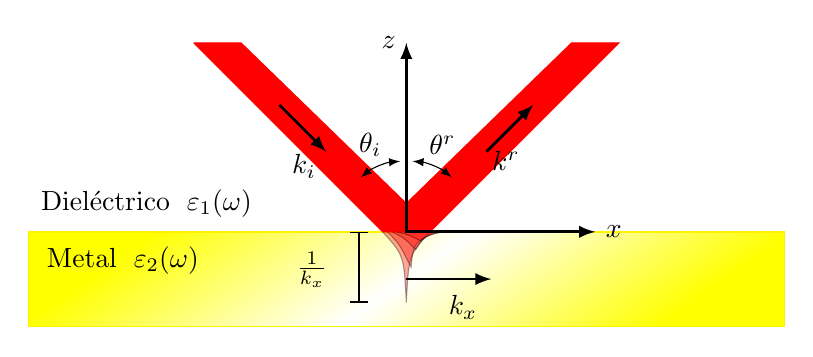
\begin{tikzpicture}[scale=1.2]
	%-------------------------------------------- Incidence media
\shadedraw[	top color = yellow,				%%%%	Color de arriba
			bottom color =yellow,				%%%%	Color de abajo
			middle color = white, 			%%	Color de en medio
			shading angle = 35]			%%%%	Ángulo de gradiente
		 (-4,-1) rectangle (4,0);
% Interface
\draw[yellow,line width=.5pt](-4,0)--(4,0)--(4,-1)--(-4,-1)--(-4,0); %%..5pt, interface]
% Media names
\node at (-2.75,.3) {Diel\'ectrico $\; \varepsilon_1(\omega)$}; 
\node at (-3,-.3) {Metal  $\; \varepsilon_2(\omega)$};

%-------------------------------------------- Laser beam outside
\draw[fill=red, opacity = 1,red](-2.25,2)--(-1.75,2)-- (0,.3)  %%% outside the metal
						--(1.75,2)--(2.25,2)
						--(.25,0)--(-.25,0)--(-2.25,2);																														
%--------------------------------------------  Incident Wave
\path (0,0)++(112.5:1cm)node{$\theta_i$};       % Angle
\draw[latex - latex](95:.75cm)arc(95:130:.75cm);
 
    \draw[- latex,line width=1pt](135:1.9cm)--(135:1.2cm);    %Wave vector
    \path (0,0)++(141:1.1cm)node[left]{$\vb{k}_i$};     %Wave vector label
    
%--------------------------------------------  Reflected Wave
\path (0,0)++(67.5:1cm)node{$\theta^r$};       % Angle
\draw[latex - latex](85:.75cm)arc(85:50:.75cm);
 
    \draw[- latex,line width=1pt](45:1.2cm)--(45:1.9cm);    %Wave vector
    \path (0,0)++(43:1.1cm)node[right]{$\vb{k}^r$};     %Wave vector label
  
%--------------------------------------------  Transmitted Wave & Skin depth
\draw[fill = red, opacity = .35] (-.25,0) ..controls (-.025,-.25) .. (0,-.75)
											..controls (.025,-.25) .. (.25,0);  %1st evanescent wave
\draw[fill = red, opacity = .35] (-.2,0) ..controls (-.075,-.125) .. (0.05,-.375)
											..controls (.075,-.125) .. (.3,0);  %2nd evanescent wave
\draw[fill = red, opacity = .35] (-.15,0) ..controls (-.025,-.0625) .. (0.1,-.1875)
											..controls (.175,-.0625) .. (.35,0);  %3rd evanescent wave
\draw[fill = red, opacity = .35] (-.1,0) ..controls (.025,-.03125) .. (0.15,-.09375)
											..controls (.225,-.03125) .. (.4,0);  %4th evanescent wave	

    \draw[- latex,line width=1pt](0,-.5)--(.9,-.5);    %Wave vector
    \node at (.6,-.8) {$\vb{k}_x$};
    
    \draw[|-|,line width=.2mm,black] (-.5,.0)--(-.5,-.75);%
    \node at (-1,-.4) {$\frac{1}{k_x}$};
%--------------------------------------------  Axes
\draw[latex - latex, line width =1pt] (0,2)node[left]{$z$}--(0,0) -- (2,0)node[right]{$x$};
\end{tikzpicture}
	\caption{ Esquema de la interfaz entre un medio dieléctrico y un medio metálico; ambos homogéneos, lineales e isótropos. Un haz de luz incide en el metal desde el medio dieléctrico.  La reflexión es total debido a la naturaleza metálica del material sin embargo, se presenta una onda evanescente que se propaga en dirección paralela a la interfaz.}\label{fig:SPP}
	\end{figure}
	
En la Fig. \ref{fig:SPP} se observa en el medio metálico, $z<0$, se presenta una onda evanescente que se propaga en la dirección $\vu{e}_x$, cuya amplitud decae exponencialmente y cuyo máximo valor $1/k_x$ es la longitud de penetración, con $k_x$ la componente paralela a la interfaz del vector de onda. Los campos EMs de la onda evanescente se proponen como 

	\begin{subequations}\eqhalf{	\vb{E}(\vb{r},t) = \vb{E}(z)e^{ik_x x-\omega t },}
	\eqhalf{\vb{H}(\vb{r},t) = \vb{H}(z)e^{ik_x x-\omega t},}
	\label{eq:EHbetax}\end{subequations}
	
\noindent Si $z>0$, entonces $\vb{E}(z)=\vb{E}_1$, con $E_1$ la magnitud de del campo eléctrico dentro del dieléctrico, y si $z<0$, entonces $\vb{E}(z)=\vb{E}_2$, la magnitud de del campo eléctrico en el medio metálico; la misma distinción se hace para el campo $\vb{H}$ y para la función dieléctrica $\varepsilon(z)$. Dado que los campos EMs cumplen con la ecuación de Helmholtz [Ec. \eqref{eq:Helmholtz}], al sustituir las expresiones de las Ecs. \eqref{eq:EHbetax}, se obtiene

	\begin{subequations}
	\eqhalf{	\pdv[2]{\vb{E}}{z} + \qty[k_0^2\frac{\varepsilon(z)}{\varepsilon_0} - k_x^2 ] \vb{E}= 0,\label{eq:helmE}}
	\eqhalf{\pdv[2]{\vb{H}}{z} + \qty[k_0^2\frac{\varepsilon(z)}{\varepsilon_0}  - k_x^2 ] \vb{H}= 0, \label{eq:helmH}}
	\end{subequations} 
	
\noindent en donde $k_0 = \omega/c$.	La polarización de la onda plana incidente interviene en la relación de dispersión del SPP, por lo que se calcularan los los campos EMs para las polarizaciones \emph{s} y \emph{p}. Se considera, además, que  hay homogeneidad en la dirección $y$ y que la única dependencia en la variable $x$  es en el término de propagación, es decir, que $\partial/\partial x\to ik_x$. Bajo estas consideraciones, al desarrollar la ley de Faraday-Lenz y la ley de Ampère-Maxwell con las expresiones de las Ecs. \eqref{eq:EHbetax} se obtiene el conjunto de ecuaciones

	\begin{subequations}
	\eqhalf{	\mqty(-\pdv*{E_y}{z} \\ \pdv*{E_x}{z}-ik_x E_z\\ik_x E_y)
				= i\omega\mu_0 \mqty(H_x\\H_y\\h_z),}
	\eqhalf{	\mqty(-\pdv*{H_y}{z} \\ \pdv*{H_x}{z}-ik_x H_z\\ik_x H_y)
				= i\omega\varepsilon(z) \mqty(E_x\\E_y\\E_z).}	
	\end{subequations}\noindent 

En la configuración de polarización \emph{s}, las componentes no nulas de los campos EM son $E_y$, $H_z$ y $H_x$, por los campos EMs cumplen con las relaciones

	\begin{subequations}
	\eqhalf{	H_x =  \frac{i}{\omega \mu_0} \pdv{E_y}{z},\label{eq:Hx}}
	\eqhalf{H_z =  \frac{q}{\omega \mu_0} E_y, \label{eq:Hz}}	
	\label{eq:ondaS}	\end{subequations} 

\noindent además de la Ec. \eqref{eq:helmE} con $\vb{E} = E_y\vu{e}_y$, cuya solución se propone como
	\begin{align}
	E_y(z) = \begin{dcases}
		E_1 e^{ik_x x} e^{-k_{1,z}z}, & z>0,\\
		E_2 e^{ik_x x} e^{k_{2,z} z}, & z<0,
		\end{dcases}\label{eq:AnsatzEy}
	\end{align}
con $k_{j,z} = k_j\cos\theta_i$ y $k_j = k_0 \sqrt{\varepsilon_j(\omega)/\varepsilon_0}$, con $j = 1,2$; donde se escribe de forma explícita el comportamiento de decaimiento exponencial en la amplitud y se omite el término $e^{-i\omega t}$ por simplicidad. Se impone que $\Re[\sqrt{\varepsilon_j(\omega)}] >0$, para que la amplitud de los campos EMs ---y por tanto la energía--- sea una cantidad acotada. Al calcular el campo $\vb{H}$ con las Ecs. \eqref{eq:ondaS} y \eqref{eq:AnsatzEy}, se obtienen a las expresiones 
	
	\eqhalf{	H_x(z) = \begin{dcases}
	-i \frac{E_1}{\omega\mu_0}k_{1,z} e^{ik_x x} e^{-k_{1,z} 	z}, & z>0,\\
	i \frac{E_2}{\omega\mu_0}k_{2,z} e^{ik_x x} e^{k_{2,z} z}, & z<0,
	\end{dcases}\notag}
	\eqhalf{	H_z(z) = \begin{dcases}
	\frac{E_1}{\omega\mu_0}k_x  e^{ik_x x} e^{k_{1,z} z} & z>0,\\
	\frac{E_2 }{\omega\mu_0}k_x  e^{ik_x x} e^{k_{2,z}z} & z<0.
	\end{dcases}\notag}
	
\noindent   Las condiciones a la frontera de los campos EMs imponen que la componente paralela a la interfaz del campo eléctrico, $E_y$, y del campo$\vb{H}$, $H_z$, sean continuas, por lo que $E_1 = E_2$. Adicionalmente, por la continuidad de la componente paralela a la interfaz del  campo $\vb{H}$, $H_x$, se concluye que
	\begin{align}
	E_1\qty(k_{1,z}+k_{2,z})= E_1 k_0\cos\theta_i \qty[\sqrt{\frac{\varepsilon_1}{\varepsilon_0}} + \sqrt{\frac{\varepsilon_2}{\varepsilon_0}}] = 0. \label{eq:condS}
	\end{align}
Por el \emph{Ansatz} propuesto en la Ec. \eqref{eq:AnsatzEy} se cumple que $\Re[\sqrt{\varepsilon_j(\omega)}]$, por tanto, la Ec. \eqref{eq:condS} se satisface si $E_1 = E_2 = 0$, es decir  que no existe un acoplamiento entre los electrones libres del metal en la interfaz plana y la onda EM incidente para polarización \emph{s}.

El cálculo de la relación de dispersión del SPP cuando incide una onda plana con polarización \emph{p} es análogo al cálculo con polarización \emph{s} al intercambiar el campo eléctrico por el campo $\vb{H}$ y al intercambiar la permitividad magnética por la función dieléctrica, es decir, $\vb{E}\leftrightarrow\vb{H}$ y $\varepsilon(z)\leftrightarrow\mu_0$. Al considerar las condiciones de continuidad del campo $\varepsilon(z)\vb{E}$ y el campo $\vb{H}$ se llega a la condición
	\begin{align}
	\frac{k_{1,z}}{k_{2,z}} = - \frac{\varepsilon_1}{\varepsilon_2}. \label{eq:condP}
	\end{align}
Asimismo, la ecuación de Helmholtz para el campo $\vb{H}$ [Ec. \eqref{eq:helmH}] impone que
	\begin{align}
	k_{j,z}^2 = k_x^2 - k_0^2 \frac{\varepsilon_j}{\varepsilon_0}.
	\label{eq:kdkm}
	\end{align}
Al elevar al cuadrado la Ec. \eqref{eq:condP}, sustituir con la Ec. \eqref{eq:kdkm}, y  despejar $k_x$  empleando la identidad de diferencia de cuadrados,  se calcula la relación de dispersión del SSP. Adicionalmente, como  $k_0^2 \varepsilon_j(\omega)= k_x^2 +k_{j,z}^2$, entonces\vspace*{-.75em}\begin{subequations}
	\begin{tcolorbox}[title = Relación de dispersión del SPP, breakable ]
	\eqhalf{k_x^2 = \frac{k_0^2}{\varepsilon_0} \frac{\varepsilon_1 \varepsilon_2}{\varepsilon_1 + \varepsilon_2},
	\label{eqs:kx}}
	\eqhalf{	k_{j,z}^2 = \frac{k_0^2}{\varepsilon_0} \frac{\varepsilon_j^2}{\varepsilon_1 + \varepsilon_2},}
	
	con $j=1$, el medio dieléctrico; y $j=2$, el medio metálico.
	\end{tcolorbox}\label{eq:SPPRelDiso}\end{subequations}\vspace*{-.75em}
\noindent La frecuencia de resonancia $\omega$ del SPP se encuentra cuando la Ec. \eqref{eqs:kx} es máxima, es decir, cuando $\varepsilon_1(\omega)+\varepsilon_2(\omega)$ es mínima. Si se emplea el modelo de Drude-Sommerfeld [Ec. \eqref{eq:Drude}] en el límite $\gamma\ll\omega$, entonces  \vspace*{-.75em}
	\begin{tcolorbox}[title =Frecuencia de resonancia del SPP, ams align,  breakable ]
	\omega = \frac{\omega_p}{\sqrt{1+\varepsilon_1/\varepsilon_0}}.
	\end{tcolorbox}\vspace*{-.75em}\noindent

\begin{figure}[h!]\centering
	\begin{tikzpicture}
	\node[inner sep=0pt] at (0,0)
    {\includegraphics[scale=1]{1-Teoria/figs/1-4-RelacionDispersion.pdf}};
    \draw [thick, decorate, decoration={brace,amplitude=10pt,mirror}]
(6.5,-.8) -- (6.5,4.0);
\node at (8,2.5){\footnotesize Modo};
\node at (8,2.){\footnotesize radiativo};
\node at (8,1.5){\footnotesize $k_x\to\text{Real}$};
\node at (8,1.){\footnotesize $k_z\to\text{Real}$};
    \draw [thick, decorate, decoration={brace,amplitude=10pt,mirror}]
(6.5,-3.25) -- (6.5,-1.3);
\node at (8,-1.5){\footnotesize Modo};
\node at (8,-2.){\footnotesize ligado};
\node at (8,-2.5){\footnotesize $k_x\to\text{Real}$};
\node at (8,-3.){\footnotesize $k_z\to\text{Imaginario}$};
\end{tikzpicture}
\vspace*{-1em}
	\caption{Relación de dispersión en términos de $\omega/\omega_p$ como función de $k_xc/\omega_p$ de una onda plana en vacío (línea sólida negra), del plasmón de volumen (línea sólida roja) y del SPP (líneas sólida azul) para materiales con una función dieléctrica tipo Drude en el límite $\gamma\ll\omega$ y sobre una interfaz con el vacío ($\varepsilon_1 =\varepsilon_0$). El régimen de modos radiativos se encuentra en $\omega_p\leq\omega$ (igualdad denotada por la línea punteada roja), donde $k_x$ y $k_z$ son cantidades reales; el régimen de modos ligados se encuentra en $\omega\leq\omega_p/\sqrt{2}$ (igualdad denotada por la línea punteada azul), donde $k_x$ es una cantidad real pero $k_z$ es una cantidad imaginaria. Para excitar a SPP es necesario cambiar el índice de refracción de la matriz, por ejemplo empleando un prisma para obtener una onda plana viajando en vidrio(línea punteada negra); la región sombreada delimita las frecuencias a las que el SPP puede excitarse.}
	\label{fig:Relaciones_de_dispersion}
	\end{figure}	


La Fig. \ref{fig:Relaciones_de_dispersion} muestra la relación de dispersión como la dependencia de la frecuencia $\omega$ como función de la componente paralela del vector de onda $k_x$ respecto a una interfaz entre el vacío ($\varepsilon_1=\varepsilon_0$) y un material descrito por le modelo de Drude-Sommerfeld [Ec. \eqref{eq:Drude}] en el límite $\gamma\ll\omega$ para una onda plana  (línea continua negra), para el plasmón de volumen (línea continua roja) y para un SPP (línea continua roja). Las líneas discontinuas roja y azul corresponden a los valores $\omega=\omega_p$ y $\omega=\omega_p/\sqrt{2}$, respectivamente, que son valores de omega que delimitan el régimen de modos radiativos ($\omega>\omega_p$), donde las dos componentes del vector de onda $\vb{k}$ son cantidades reales, y el régimen de modos ligados ($\omega<\omega_p/\sqrt{2}$), donde $k_x$ es una cantidad real pero la componente del vector de onda perpendicular a la interfaz $k_z$ es una cantidad imaginaria. Las líneas continua negra y discontinua negra corresponden a la relación de dispersión de una onda plana propagándose en el vacío y en un medio con $n=1.5$, respectivamente.

	

Dado que la relación dispersión de la onda plana propagándose en el vacío (línea continua negra en la Fig. \ref{fig:Relaciones_de_dispersion}) no es igual a la del SPP (línea continua azul) para valores distintos de $k_x=0$, no es posible excitar al SPP con este tipo de ondas, dado que el momento de la onda plana incidente es menor al del SPP \cite{trugler2011properties}. Sin embargo, es posible complementar el momento faltante para excitar al SPP al emplear un tercer medio (dieléctrico) con un índice de refracción mayor al del dieléctrico que forma la interfaz con el medio metálico donde se excitará el SPP \cite{trugler2011properties}. Experimentalmente es posible excitar al SPP sobre la interfaz formada por una placa metálica con una función dieléctrica $\varepsilon_2(\omega)$ y la matriz dieléctrica donde se encuentra inmersa con $\varepsilon_1(\omega)$ al emplear una configuración de reflexión total atenuada (Atenuatted Total Reflexión, ATR) \cite{kabashin2009plasmonic}, en donde una onda evanescente interactúa con un objeto \cite{hecht1998optics}, como puede ser una segunda interfaz o bien, NPs soportadas sobre el sustrato. En la Fig. \ref{fig:ATR} se muestra una configuración en ATR al colocar la placa metálica inmersa en un dieléctrico sobre un sustrato cuya función dieléctrica $\varepsilon_3(\omega)$ cumpla con $\varepsilon_3(\omega)>\varepsilon_1(\omega)$. Cuando un haz de luz incide la interfaz entre la placa metálica y el sustrato, se produce una onda evanescente que se propaga en la dirección $\vb{k}_x=k_x\vu{e}_x$ y si la longitud de penetración $1/k_x$ es mayor a la altura de la placa metálica, ésta penetra la interfaz entre la matriz y la placa que permite excitar al SPP sobre esta interfaz \cite{trugler2011properties}. 	
	
\begin{figure}[h!]\centering
	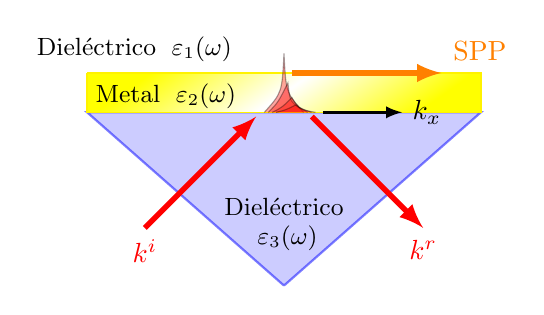
\begin{tikzpicture}
%-------------------------------------------- Incidence media
\def\a{.3}
\def\d{.3}
\def\dd{.2}
\def\l{2.5}

\fill[blue, opacity = .2] (0,-\l)--(\l,-\d)--(-\l,-\d);
\draw[blue, opacity = .5,thick] (0,-\l)--(\l,-\d)--(-\l,-\d)--(0,-\l);


%
%\foreach \x in {-4,-2.9,-1,.1,1.2,2.4,3.8}{
%\fill[ball color=yellow, opacity=1] (\x,0) circle(\a);}

\shadedraw[	top color = yellow,				%%%%	Color de arriba
			bottom color =yellow,				%%%%	Color de abajo
			middle color = white, 			%%	Color de en medio
			shading angle = 35]			%%%%	Ángulo de gradiente
		 (-\l,-\d) rectangle (\l,\dd);
% Interface
\draw[yellow,line width=.5pt](-\l,\dd)--(\l,\dd)--(\l,-\d)--(-\l,-\d)--(-\l,\dd); %%..5pt, interface]

% Media names
\node at (0,-1.5) {\small Diel\'ectrico}; 
\node at (0,-1.9) {\small $\; \varepsilon_3(\omega)$}; 
\node at (-1.5,-.1) {\small Metal  $\; \varepsilon_2(\omega)$};
\node at (-1.9,.5) {\small Diel\'ectrico $\; \varepsilon_1(\omega)$}; 

%\draw[thick, dashed] (-4.5,0)--(4.5,0);
%\draw[thick, dashed] (-4.5,-\d) rectangle (4.5,\d);

\draw[latex -, thick, red, line width = 2](225:.5)--(225:2.5) node[anchor= north]{$\vb{k}^i$};
\draw[- latex, thick, red, line width= 2](-45:.5)--(-45:2.5)node[anchor=north ]{$\vb{k}^r$};
\draw[- latex, thick,   line width = 1](.5,-\d)--(1.5,-\d) node[anchor= west ]{$\vb{k}_x$};
\draw[- latex, thick, orange,  line width = 2](.1,\dd)--(2,\dd) node[anchor= south west ]{SPP};



\draw[fill = red, opacity = .35] (-.25,-\d) ..controls (-.025,.25-\d) .. (0,.75-\d)
											..controls (.025,.25-\d) .. (.25,-\d);  %1st evanescent wave
\draw[fill = red, opacity = .35] (-.2,0-\d) ..controls (-.075,.125-\d) .. (0.05,.375-\d)
											..controls (.075,.125-\d) .. (.3,0-\d);  %2nd evanescent wave
\draw[fill = red, opacity = .35] (-.15,0-\d) ..controls (-.025,.0625-\d) .. (0.1,.1875-\d)
											..controls (.175,.0625-\d) .. (.35,0-\d);  %3rd evanescent wave
\draw[fill = red, opacity = .35] (-.1,0-\d) ..controls (.025,.03125-\d) .. (0.15,.09375-\d)
											..controls (.225,.03125-\d) .. (.4,0-\d);  %4th evanescent wave	

\end{tikzpicture}	
	\caption{ Esquema de la configuración ATR para una placa metálica con una función dieléctrica $\varepsilon_2(\omega)$ inmersa en una matriz dieléctrica con $\varepsilon_1(\omega)$ y sobre un prisma dieléctrico con $\varepsilon_3(\omega)>\varepsilon_1(\omega)$. Cuando un haz de luz con polarización \emph{p} incide sobre la interfaz entre el prisma y la placa de metal se produce una onda evanescente propagante en la dirección $\vb{k}_x=k_x\vu{e}_x$; si la longitud de penetración $1/k_x$ es mayor a la altura de la placa metálica, es posible excitar al SPP sobre la interfaz entre el medio metálico y el vacío, como se observa en la Fig. \ref{fig:Relaciones_de_dispersion} con el cruce la línea discontinua negra (onda plana viajando en un dieléctrico con $n=1.5$) y la línea continua azul (SPP propagándose en la interfaz entre el vacío y un material descrito por le modelo de Drude-Sommerfeld con $\gamma\ll\omega$).}
	\label{fig:ATR}
	\end{figure}
		
El SPP es un acoplamiento de los electrones libres sobre la interfaz entre un dieléctrico y un material metálico y es una solución a las ecuaciones de Maxwell que se propaga a través de la interfaz plana que se considera infinita. Cuando la interfaz tiene una área finita, como sucede con las NPs esféricas, el resultado no es una onda propagante, sino 


	El campo esparcido [Ec.  \eqref{eq:Es}] está en términos de los coeficientes $a_\ell$ y $b_\ell$ [Ecs.  \eqref{eq:MieCoef}], que dependen, entre otros parámetros, del índice de refracción de la partícula.  De la Ec.  \eqref{eq:Es} se observa que, para un multipolo $\ell$ fijo, la contribución del campo eléctrico es máxima cuando el denominador de los coeficientes de Mie es mínimo \cite{novotny2006principles}.  Si se considera que la respuesta óptica de la partícula es 	$\varepsilon_p (\omega) = n_p^2 (\omega)$, y se fijan los parámetros $a$, $n_m$ y $\lambda$, 	entonces a la frecuencia $\omega_\ell = c (2\pi / \lambda_\ell)$, donde el denominador de las Ecs.  \eqref{eq:MieCoef} es nulo, se le denomina \emph{modo normal} de orden $\ell$ \cite{bohren1998absorption,maciel2017momentum}.  Los modos normales eléctricos ocurren a las frecuencias en las que se cumple la condición 
	\begin{align}
	\psi_\ell(mx)\xi_\ell'(x)-m\xi_\ell(x)\psi_\ell'(mx) = 0. 
	\label{eq:an_resonance}
	\end{align}
Al considerar el límite de partícula pequeña ($x\ll 1$) para esferas inmersas en vacío ($n_m=1$), haciendo un desarrollo en serie de Taylor de las funciones de Bessel y Hankel alrededor del origen y sustituyéndolas en la Ec.  \eqref{eq:an_resonance}, se obtiene que los modos normales eléctricos cumplen la relación \cite{maciel2017momentum}
	\begin{align}
	\varepsilon_p(\omega_\ell) = - \frac{\ell+1}{\ell}.  
	\label{eq:NormalModes}
	\end{align}

	\begin{figure}[h!]\centering
		\includegraphics[scale=1]{1-Teoria/figs/1-4-DrudeMultipoles.pdf}\vspace*{-1em}
	\caption{Frecuencias de resonancia $\omega_\ell/\omega_p$ para una esfera con una función dieléctrica tipo Drude, como función del parámetro adimensional  $\omega_p a / c$, para los multipolos $\ell = 1,2,3$ y $4$. }
	\label{fig:NormalModes}
	\end{figure}			
	
Si se emplea la función dieléctrica del modelo de Drude-Sommerfeld [Ec.  \eqref{eq:Drude}] para $\omega = \omega_\ell$	y se sustituye en la Ec.  \eqref{eq:NormalModes}, al despejar $\omega_\ell$ tras considerar además el límite $\gamma\to 0$, la expresión para la frecuencia de resonancia del  modo normal del multipolo $\ell$ es \cite{maciel2017momentum}
	\begin{align}
	\frac{\omega_\ell}{\omega_p} = \sqrt{ \frac{\ell}{2\ell+1}}. \label{eq:PPequeña}
	\end{align}
Adicionalmente, si se considera la contribución de todos los órdenes multipolares ($\ell\to \infty$), la mayor frecuencia de resonancia es $\omega_\infty = \omega_p/\sqrt{2}$, que corresponde a la SPR de superfice.	
	
Para partículas esféricas de radio arbitrario $a$ con una función dieléctrica dada por el modelo de Drude-Sommerfeld, la frecuencia de resonancia $\omega_\ell$ sufre un corrimiento al rojo debido al tiempo de acomplamiento $a/c$ entre la interacción EM de la esfera y  la densidad de carga inducida que corresponde al plasmón de superficie \cite{aizpurua1998coupling}.  En la Fig.  \ref{fig:NormalModes} se muestran las frecuencias de resonancia $\omega_\ell$ normalizadas respecto a la frecuancia de plasma $\omega_p$, como función del parámetro adimensional $a\omega_p / c$ para los multipolos $\ell = 1,2,3$ y $4$.  El límite de partícula pequeña [Ec.  \eqref{eq:PPequeña}]	se recupera cuando  $a\to 0$ (lado izquierdo de la gráfica en la Fig.  \ref{fig:NormalModes}).  Para una función dieléctrica arbitraria, los modos normales se calculan como la frecuencia a la que la partícula extingue\footnote{Extinción se entiende como la pérdida de luz ocacionada por la absorción y esparcimiento de luz de la partícula; esta relación es conocida como el  \emph{teorema óptico} \cite{bohren1998absorption}. } la mayor cantidad de luz \cite{kreibig1995clusters}. 


\section{Modelo de esparcimiento coherente}


La solución de Mie, en conjunto con la corrección por tamaño de la función dieléctrica para algún material, permite estudiar la respuesta electromagnética (EM) de una nanopartícula (NP) esférica individual, tales como los plasmones localizados de superficies (Localized Surface Plasmons, LSPs), lo cuales son empleados en la espectroscopía \cite{novotny2006principles}, el sensado \cite{jain2008noble}, la litografía \cite{stockman2011nanoplasmonics}. Sin embargo, no siempre es posible emplear la respuesta EM de una partícula individual para la descripción del sistema por lo que se han empleado diversos enfoques entre los que se encuentran la aproximación cuasiestática y las teorías de esparcimiento \cite{pena-gomar2006coherent}. En el caso límite de partícula pequeña, donde el parámetro de tamaño $x=ka= 2\pi n_m$, con $n_m$  el índice de refracción del medio donde se encuentra inmersa NP, es mucho menor que la unidad, es posble emplear  la aproximación cuasiestática, que considera que sólo la excitación dipolar contribuye al campo total. En partícular, para la reflectancia de una monocapa de NPs, la aproximación cuasiestática conduce a una teoría de medio efectivo \cite{pena-gomar2006coherent}. Sin embargo, cuando  el parámetro de tamaño es comparable o mayor a la unidad, una teoría de esparcimiento es necesaria, debido a la inducción de multipolos de ordenes mayores \cite{pena-gomar2006coherent}. El modelo de esparcimiento coeherente (CSM) toma en cuenta la interacción de esparcidores puntuales ante la presencia de un campo eléctrico promedio; este acercamiento además incluye la contribución del esparcimiento múltiple debido a la interacción entre las NPs.
    
    El cálculo de las expresiones de reflectancia y transmitancia en el formalismo del CSM considera el campo eléctrico total esparcido por una monocapa de NPs. En general, éste puede descomponerse en una componente coherente ---respuesta promedio con una dirección de propagación bien definida--- y una componente difusa ---causada por las fluctuaciones y cuya propagación es en todas las direcciones--- \cite{tsang2000scattering}. Para definir los coeficientes de amplitud de reflexión y transmisión de la manera usual, se toma en cuenta  únicamente la componente coherente al asumir que la difusa es mucho menor que la coherente. Asimismo, primero se calculan los coeficientes de amplitud de reflexión y transmisión de una monocapa de NPs suspendida en el espacio libre (Free Standing Monolayer, FSM), es decir, inmersa en un medio dieléctrico denominado matriz, seguido del efecto de introducir una interfaz con un medio denominado sustrato. La reflectancia del sistema sustrato-matriz-monocapa se resuelve al considerar  multiples reflexiones en la interfaz entre las superficies dadas por la interfaz sutrato-matriz y matriz-monocapa. Este acercamiento evita el  cálculo de la contribución de partículas \emph{imagen} causadas por la  interfaz entre los dieléctricos y es consistente con la aproximación de campo efectivo ---en donde el campo eléctrico local es aproximado por el campo eléctrico promedio--- \cite{reyes2018analytical}.
 
\subsection{Monocapa suspendida en el espacio libre}
 
Para calcular los coeficientes de amplitud de reflexión y transmisión del CSM se calcula el campo eléctrico promedio esparcido por las NPs dentro de la región del espacio, caracterizado en su totalidad por el índice de refracción real $n_m$, delimitada por  $-d/2<z<d/2$, una placa de longitud $d$ y volumen $V$, en donde se encuentran $N$ NPs esféricas e idénticas y distribuidas espacialmente de forma aleatoria. Si una onda plana $\vb{E}^i = E_0 e^{i\vb{k}^i\cdot\vb{r}}\vu{e}_i$, donde se omite la dependecia temporal, y donde $\vu{e}_i$ es un vector en el plano de polarización de la onda plana y $|\vb{k}^i| = k = 2\pi n_m /\lambda$, incide sobre la placa, el campo eléctrico esparcido  por las NPs dentro de la placa $\vb{E}^s$, al suponer que la densidad $N/V$ es baja, puede calcularse bajo la aproximación de esparcidor individual (Single Scatterer Approximation, SSA), en donde cada NP esparce la luz sin considerar la interacción entre el campo eléctrico esparcido por las otras \cite{barrera2003coherent}. 

\begin{figure}[h!]\centering
	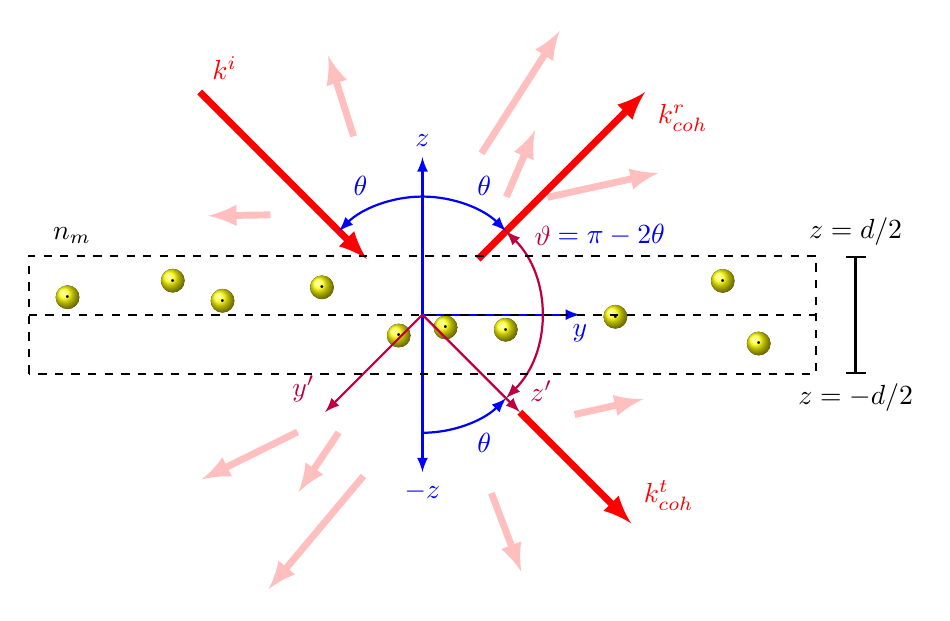
\begin{tikzpicture}[scale=1]
\def\a{.15}
\def\d{.75}
%----------------------NPs--------------
\foreach \y in {-4.5,-3.5,...,3.5,4.5}{
\fill[ball color=yellow, opacity=1] (\y+rand*.5,rand*.45) circle(\a) node[ ]{.};
}

%----------------------difussed scattered field--------------
\begin{scope}[opacity=.25, transparency group]
\foreach \s in {-1,1}{
	\draw[- latex, red, line width=2.5](0,\s*\d)++(25:\s*1.75)--(35+rand*5:\s*3.5);
	\draw[- latex, red, line width=2.5](0,\s*\d)++(35:\s*1.3)--(55+rand*5:\s*2.75);
	\draw[- latex, red, line width=2.5](0,\s*\d)++(165:\s*2)--(155+rand*5:\s*3);
	\draw[- latex, red, line width=2.5](0,\s*\d)++(120:\s*1.75)--(110+rand*5:\s*3.5);
	\draw[- latex, red, line width=2.5](0,\s*\d)++(60:\s*1.5)--(60+rand*5:\s*4);}
\end{scope}

%----------------------coherent scattered field--------------
\draw[latex -, thick, red, line width=2.5](135:1)--(135:4) node[anchor=south west]{$\vb{k}^i$};
\draw[- latex, thick, red, line width=2.5](45:1)--(45:4)node[anchor=north west]{$\vb{k}_{coh}^r$};
\draw[ - latex, thick, red, line width=2.5](-45:1.75)--(-45:3.75) node[anchor=south west]{$\vb{k}_{coh}^t$};

%----------------------Main system--------------
\draw[- latex, thick, blue] (0,0)--(90:2) node[anchor = south]{$z$};
\draw[- latex, thick, blue] (0,0)--(-90:2) node[anchor = north]{$-z$};
\draw[- latex, thick, blue] (0,0)--(0:2) node[anchor = north]{$y$};
\path (0,0)++(135/2:1.5)node[anchor=south west, blue]{$\theta$}; 
\draw[- latex, thick, blue](90:1.5)arc(90:45:1.5);
\path (0,0)++(-135/2:1.5)node[anchor=north west, blue]{$\theta$}; 
\draw[- latex, thick, blue](-90:1.5)arc(-90:-45:1.5);
\path (0,0)++(90+45/2:1.5)node[anchor=south east, blue]{$\theta$}; 
\draw[- latex, thick, blue](90:1.5)arc(90:135:1.5);

----------------------Mie system--------------
\draw[- latex, thick, purple] (0,0)--(-45:1.75) node[anchor = south west]{$z'$};
\draw[- latex, thick, purple] (0,0)--(-135:1.75) node[anchor = south east]{$y'$};
\path (0,0)++(30:1.5)node[anchor=south west, purple]{$\vartheta$}; 
\path (0,0)++(30:1.5)node[anchor=south west, blue]{$\;\;\; =  \pi - 2\theta$}; 
\draw[latex - latex, thick, purple](-45:1.5)arc(-45:45:1.5);

%----------------------thickness and slab-------------
\draw[thick, dashed] (-5,-\d) rectangle (5,\d);
\draw[thick, dashed] (-5, 0) --  (5,0);
\draw[ |-|, thick,] (5.5,-\d) node[anchor = north]{$z=-d/2$} -- (5.5,\d) node[anchor = south]{$z=d/2$};
\node at (-4.5,1) {$\; n_m$};
\end{tikzpicture}
	\caption{  Película de grosor $d$ con y volumen $V$ con $N$ partículas esféricas idénticas y una onda incidente en la dirección $\vb{k}^i$. La dirección de los campos esparcidos coeherentes están dadas por $\vb{k}^r_{coh}$ y $\vb{k}^t_{coh}$. Las flechas rojas sólidas representan las componentes coehrentes del campo esparcido mientras que las rosas represetan su componente difusa. }\label{fig:CSM-Slab}
	\end{figure}


Al considerar la interacción del campo eléctrico incidente con las $N$ NPs dentro de la placa, el campo eléctrico esparcido por todas las partículas tiene componentes espaciales en todas las direcciones, por lo que le campo eléctrico esparcido puede descomponerse en una componente coherente y una difusa. El  campo eléctrico esparcido promedio $\langle \vb{E}^s\rangle$, que corresponde a la componente coherente, se calcula al considerar el promedio espacial de las NPs dentro de la placa al suponer que la posición de una NPs es independiente de la de las demás y que la probabilidad de encontrar el centro de una NPs, punto negro dentro de las NPs en la Fig. \ref{fig:CSM-Slab},  dentro del volumen de la placa es uniforme, por lo que la componente coherente del campo esparcido es  \cite{garcia2012multiple} 
	\begin{align}
	\langle \vb{E}^s\rangle =
	\begin{dcases} 
	      \langle \vb{E}^s_{r,SSA}\rangle e^{i\vb{k}^r_{coh}\cdot\vb{r}} =
	    			i \frac{N}{V}  \frac{d E_0}{2} \frac{\sin(k_z^id)}{k_z^i d} 
				\frac{\mathbb{F}(\vu{k}^r,\vu{k}^i)\cdot \vu{e}_i}{k_z^i }	e^{i\vb{k}^r_{coh}\cdot\vb{r}},									& d/2<z \\
      \langle \vb{E}^s_{t,SSA}\rangle e^{i\vb{k}^t_{coh}\cdot\vb{r}} =
 				i\frac{N}{V} \frac{d E_0}{2}\frac{\mathbb{F}(\vu{k}^i,\vu{k}^i)\cdot \vu{e}_i}{k_z^i}		
				e^{i\vb{k}^t_{coh}\cdot\vb{r}},
							& z<-d/2
   \end{dcases}
   	\label{eq:AvErEt}
	\end{align}
en donde $k^i_z = k^i\cos\theta$; $\vb{k}^i$ es el vector de onda del campo eléctrico incidente $\vb{E}^i = \vb{E}_0 e^{i\vb{k}^i\cdot\vb{r}}$, polarizado en la dirección $\vu{e}_i$; $\vb{k}^r_{coh}$ es la dirección de propagación de la componente coherente reflejada; $\vb{k}^t_{coh}=\vb{k}^i$, de la componente coherente transmitida; y $\mathbb{F}$ es la diadica de esparcimiento de campo lejano [Ec. \eqref{eq:FarFieldDyadic}] que depende de la dirección de propagación de la onda plana incidente $\vb{k}^i$ y la del campo esparcido $\vb{k}^s$; el término de $\mathbb{F}$ no limita la solución del campo eléctrico esparcido promedio al campo lejano puesto que es un resultado derivado del promediar la respuesta EM \cite{gutierrez2012overview}. En la Fig, \ref{fig:CSM-Slab} se observa que la dirección de propagación de  $\langle \vb{E}^s_{r,SSA}\rangle$ en $d/2<z$ y la de $\langle \vb{E}^s_{t,SSA}\rangle$ en  $z<-d/2$ es de $\theta$ respecto a la dirección normal a la monocapa (sitema coordenado azul). Asimismo, se muestra en rojo claro la componente difusa del campo eléctrico esparcido que, al calcular el campo esparcido promedio, es nula. A diferencia la componente difusa, la componente coherente del campo eléctrico esparcido es distinta de cero ya que los campos eléctricos esparcidos por cada NP en la placa interfieren constructivamente en las direcciones de esparcimiento $\vu{k}^s =\vu{k}^i=\vu{k}^t_{coh}$ y $\vu{k}^s =\vu{k}^r_{coh}$ \cite{garcia2012multiple}. Puesto que las NPs dentro de la placa son esféricas e idénticas, se calcula la expresión de la diadica de esparcimiento $\mathbb{F}(\vu{k}^s,\vu{k}^i)$ al comparar su expresión general [Ec. \eqref{eq:FarFieldDyadic}] con la matriz de esparcimiento de Mie [Ec. \eqref{eq:MieMatrix}], por lo que la diadica de esparcimiento de campo lejano es
	\begin{align}
	\mathbb{F}(\vu{k}^s,\vu{k}^i) = \frac{1}{-ik} 
	 \mqty(S_2(\vartheta) & 0 \\ 0 & S_1(\vartheta)),
	 \label{eq:FFDydadic-Mie}
	\end{align}
en donde ángulo entre la dirección del campo esparcido $\vu{k}^s$ y del campo incidente $\vu{k}^i$, se denota con $\vartheta$ que toma los valores $\vartheta = 0$ para $\vu{k}^s = \vu{k}^t_{coh}$ y $\vartheta = \pi-2\theta$  para $\vu{k}^s = \vu{k}^r_{coh}$ como se observa en la Fig. \ref{fig:CSM-Slab}.
	
Al sustituir la Ec. \eqref{eq:FFDydadic-Mie} en la Ec. \eqref{eq:AvErEt} y multiplicar las expresiones resultantes por $(3ka^3)/(3ka^3)$, con $a$ el radio de las NPs y $k = 2\pi n_m /\lambda$, y agrupar términos, se llegan a las expresiones 
	\begin{subequations}\begin{align}
		\langle \vb{E}^s_{r,SSA}\rangle & = - \frac{E_0}{\cos\theta_i} \frac32  \qty(\frac{N}{V} \frac43\pi a^3)\frac{kd}{(ka)^3}   \frac{\sin(k_z^id)}{k_z^i d}  S_n(\vartheta)\vu{e}_i =
		-\alpha  \frac{\sin(k_z^id)}{k_z^i d}   S_n(\vartheta) \vb{E}_0,
		\label{eqs:EsSSAr}\\
	\langle \vb{E}^s_{t,SSA}\rangle &=  - \frac{E_0}{\cos\theta_i} \frac32
						 \qty(\frac{N}{V}\frac43\pi a^3  ) \frac{kd}{(ka)^3}  S_n(0) \vu{e}_i  
						 = - \alpha S(0) \vb{E}_0
		\label{eqs:EsSSAt}
	\end{align}\label{eq:EsSSA}\end{subequations}
donde  se emplea $n=1$ para polarización $s$ y $n_2$ para $p$ en las entradas no nulas de la matriz de esparcimiento de Mie $S_n(\vartheta)$ y donde se define $S(0) \equiv S_1(0)=S_2(0)$. Al sustituir con el parámetro de tamaño $x=ka$ se obtiene que  
\begin{align*}
	\alpha \equiv \frac32 \qty(\frac{N}{V}\frac43 \pi a^3  )\frac{kd}{x^3\cos\theta_i} = \frac32\frac{kd}{ x^3\cos\theta_i} f,
	\end{align*}
con $f= N 4\pi a^3/(3V)$ la fracción de llenado que es el cociente entre el neto de las NPs entre el volumen de la placa. Si se considera el límite $d\to 0$, lo que equivale a tener una monocapa de partículas esféricas desordenadas y al asumir que la componente difusa del campo esparcido por las partículas es despreciable en comparación a la componente coherente, es posible definir los coeficientes de amplitud de reflexión y transimisión en la SSA a partir de las Ecs. \eqref{eq:EsSSA} como \vspace*{-.75em}	
	
	\begin{subequations}\eqhalf{r_{coh}^{SSA} = -\alpha S_n(\vartheta),}
	\eqhalf{t_{coh}^{SSA} = 1 - \alpha S(0), }
	\label{eq:rtcohSSA}\end{subequations}\vspace*{-.75em}	
	
\noindent en donde para el coeficiente de amplitud de transmisión se suma la contribución de la onda plana a la Ec. \eqref{eqs:EsSSAt}, y al considerar que $V = A d$, el coeficiente $\alpha$ se reescribe como
	\begin{align}
	\alpha = \frac{2\Theta}{x^2 \cos\theta_i}
	\label{eq:alpha}
	\end{align}
donde $\Theta = N \pi a^2 / A$ es la fracción de cubierta que corresponde al área proyectada por las esferas sobre el área de la placa. Al analizar  las Ecs. \eqref{eq:rtcohSSA} y \eqref{eq:alpha}, para ángulos rasantes $\theta\to \pi/2$ se observa que $\alpha\to \infty$, además de que para partículas pequeñas $x\ll 1$ el producto $r_{coh}^{SSA}r_{coh}^{SSA*}$ puede tomar valores mayores a la unidad. Por tanto los coeficientes de amplitud calculadas a partir de la SSA son válidos únicamente para ángulos de incidencia no rasantes y para partículas grandes. 

Para calcular coeficientes de amplitud a partir de la SSA pero que no estén límitados a ángulos de incidencia bajos ni al tamaño de las partículas que conforman a la monocapa, se deben considerar contribuciones de esparcimiento múltiple (Multiple Scattering, MS) en el cálculo del campo eléctrico $\vb{E}^{exc}$  que excita a las partículas dentro de la placa, el cual se puede descomponer como 
	\begin{align}
	\vb{E}^{exc} = \vb{E}^{exc}_{t} e^{i\vb{k}^t_{coh}\cdot\vb{r}}+
					\vb{E}^{exc}_{r} e^{i\vb{k}^r_{coh}\cdot\vb{r}}
	\end{align}
donde  $\vb{E}^{exc}_t$ tiene la misma polarización y dirección de propagación de $\langle \vb{E}^s_{t,SSA}\rangle$  y $\vb{E}^{exc}_{r}$, de $\langle \vb{E}^s_{r,SSA}\rangle$, de las Ecs. \eqref{eq:EsSSA}, como se observa en la Fig. \ref{fig:MScatt-slab-MS}. Entonces, el campo eléctrico esparcido promedio considerando el MS $\vb{E}^s_{MS}$, toma en cuenta  las reflexiones y transmisiones de $\vb{E}^{exc}$ según las Ecs. \eqref{eq:EsSSA} en el límite $d\to 0$ \cite{gutierrez2012overview}, y la contribución del campo eléctrico incidente $\vb{E}^i$, por lo que  \cite{reyes2018analytical}
	\begin{subequations}\begin{align}
		\langle \vb{E}^s_{r,coh}\rangle & =	\langle \vb{E}^s_{r,MS}\rangle
					= \qty[-\alpha S_n(\vartheta)E^{exc}_t -\alpha S(0)E^{exc}_r
					]\vu{e}_i e^{i\vb{k}^r_{coh}\cdot\vb{r}},\\
		\langle \vb{E}^s_{t,coh}\rangle & =\vb{E}^i+\langle\vb{E}^s_{r,MS}\rangle
					= \qty[E_0 -\alpha S(0)E^{exc}_t 
					-\alpha	 S_n(\vartheta)E^{exc}_r
					]\vu{e}_i e^{i\vb{k}^t_{coh}\cdot\vb{r}}.
	\end{align} \label{eq:EsMS}\end{subequations}

	\begin{figure}[h!]\centering
		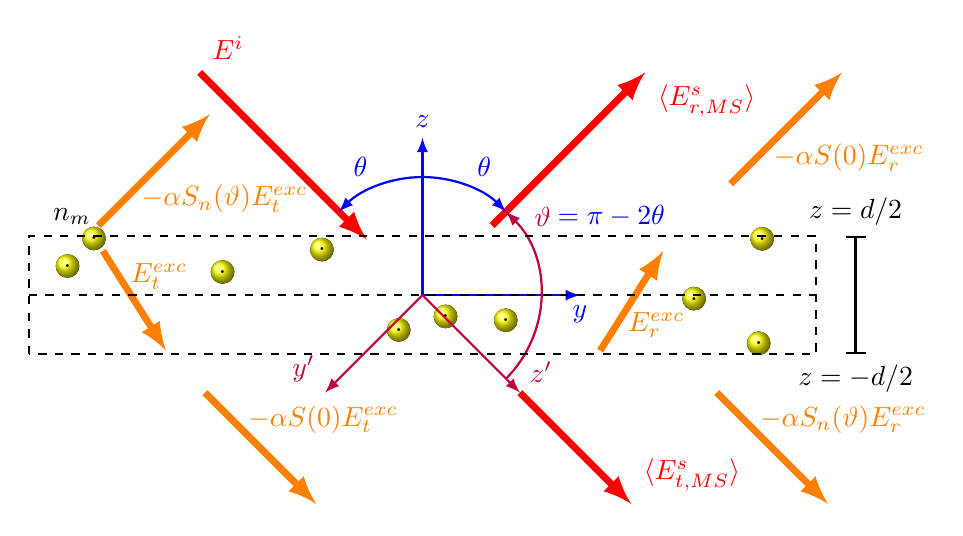
\begin{tikzpicture}[scale=1]
\def\a{.15}
\def\d{.75}

%----------------------NPs--------------
\foreach \y in {-4.5,-4.5,-2.5,-1.5,-.5,.5,1.5,3.5,4,4.5}{
\fill[ball color=yellow, opacity=1] (\y+rand*.5,rand*\d) circle(\a) node[ ]{.};
}

%----------------------averged fields ---------------------
\draw[latex -, thick, red, line width=2.5](135:1)--(135:4) node[anchor=south west]{$\vb{E}^i$};
\draw[- latex, thick, red, line width=2.5](45:\d+.5)--(45:4)node[anchor=north west]{$\langle\vb{E}_{r,MS}^s\rangle$};
\draw[ - latex, thick, red, line width=2.5](-45:1.75)--(-45:3.75) node[anchor=south west]{$\langle\vb{E}_{t,MS}^s\rangle$};

%---------------------- Exciting fields ---------------------
\draw[- latex , thick,  orange, line width=2.5,shift ={(-3,0)}](152:1.2)node[anchor= north west]{$\;\;\vb{E}^{exc}_t$}--(250:\d);
\draw[latex - , thick, orange, line width=2.5,shift ={(2,0)}](28:1.2)--(-70:\d) node[anchor= south west]{$\;\;\vb{E}^{exc}_r$};

%-------------- reflected and transmitted exciting fields UP ---------------------
\draw[latex - , thick, orange, line width=2.5,shift={(2.5, 0)}](-45:3.75)--(-45:1.75) node[anchor=north west]{$\;\;\;\;-\alpha S_n(\vartheta)\vb{E}^{exc}_r$};
\draw[latex - , thick, orange, line width=2.5,shift={(-4, 0)}](-45:3.75)--(-45:1.75) node[anchor=north west]{$\;\;\;\;-\alpha S(0)\vb{E}^{exc}_t$};

%-------------reflected and transmitted exciting fields DOWN ---------------------
\draw[latex -, thick, orange, line width=2.5,shift={(2.5, 0)}](45:4)--(45:2)node[anchor=south west]{$\;\;\;\;-\alpha S(0) \vb{E}^{exc}_r$};
\draw[latex -, thick, orange, line width=2.5,shift={(-5, 0)}](45:3.25)--(45:\d+.5)node[anchor=south west]{$\;\;\;\;-\alpha S_n(\vartheta) \vb{E}^{exc}_t$};

%----------------------main system---------------------
\draw[- latex, thick, blue] (0,0)--(90:2) node[anchor = south]{$z$};
\draw[- latex, thick, blue] (0,0)--(0:2) node[anchor = north]{$y$};
\path (0,0)++(135/2:1.5)node[anchor=south west, blue]{$\theta$}; 
\draw[- latex, thick, blue](90:1.5)arc(90:45:1.5);
\path (0,0)++(90+45/2:1.5)node[anchor=south east, blue]{$\theta$}; 
\draw[- latex, thick, blue](90:1.5)arc(90:135:1.5);

%----------------------Mie system---------------------
\draw[- latex, thick, purple] (0,0)--(-45:1.75) node[anchor = south west]{$z'$};
\draw[- latex, thick, purple] (0,0)--(-135:1.75) node[anchor = south east]{$y'$};
\path (0,0)++(30:1.5)node[anchor=south west, purple]{$\vartheta$}; 
\path (0,0)++(30:1.5)node[anchor=south west, blue]{$\;\;\; =  \pi - 2\theta$}; 
\draw[- latex, thick, purple](-45:1.5)arc(-45:45:1.5);

%----------------------thickness and slab ---------------------
\draw[thick, dashed] (-5,-\d) rectangle (5,\d);
\draw[thick, dashed] (-5, 0) --  (5,0);
\draw[ |-|, thick,] (5.5,-\d) node[anchor = north]{$z=-d/2$} -- (5.5,\d) node[anchor = south]{$z=d/2$};
\node at (-4.5,1) {$\; n_m$};
\end{tikzpicture}
		\caption{  Película de grosor $d\to 0$ con y volumen $V$ con $N$ partículas esféricas idénticas y una onda incidente en la dirección $\vb{k}^i$. La dirección de los campos esparcidos coeherentes están dadas por $\vb{k}^r_{coh}$ y $\vb{k}^t_{coh}$. Las flechas rojas sólidas representan las componentes coehrentes del campo esparcido mientras que las rosas represetan su component difusa. }\label{fig:MScatt-slab-MS}
	\end{figure}	
	
	
Para determinar la expresión del campo eléctrico que excita a las NPs en la placa $\vb{E}^{exc}$ considerando el MS\footnote{El procedimiento descrito en este texto emplea un enfoque heurístico que se publicó en \cite{reyes2018analytical} sin emabargo, un enfoque más riguroso se encuentra en \cite{barrera2003coherent}.}, se divide la placa donde se encuentras las NPs en dos de grosor $d/2$, y se calcula el promedio de  $\vb{E}^{exc}$ en la interfaz entre las dos placas ($z=0$) mediante autoconsistencia, por lo que las NPs en la placa no sólo son iluminadas por el campo eléctrico incidente $\vb{E}^i$, sino también por $\vb{E}^{exc}$ \cite{reyes2018analytical}. La componente de $\vb{E}^{exc}$ que se propaga en la dirección del campo eléctrico incidente $\vb{E}^{exc}_{t}$ se calcula como el campo incidente más los campos esparcidos por las NPs es la placa superior ($0<z<d/2$) que son  igual a la suma del la transmisión del campo $E^{exc}_t$ y a la reflexión del campo $E^{exc}_r$ por la placa superior, es decir,
	\begin{subequations}\begin{align}
		\vb{E}^{exc}_t  e^{i\vb{k}^i\cdot\vb{r}}  =
				\qty[E_0  - \frac12 \qty(
					\alpha S(0)E^{exc}_t + \alpha S_n(\vartheta)E^{exc}_r
				)] e^{i\vb{k}^t_{coh}\cdot\vb{r}}  \vu{e}_i.
	\end{align}
donde el factor de $1/2$ considera que es la respuesta promedio dentro de la placa. Asimismo, el campo $\vb{E}^{exc}_{r}$ se calcula como la reflexión  del campo $E^{exc}_t$ y a la transmisión del campo $E^{exc}_r$ por la placa inferior ($-d/2<z<0$), por lo que su expresión es	
	\begin{align}
	\vb{E}^{exc}_r  e^{i\vb{k}^r\cdot\vb{r}}  =
				\qty[- \frac12 \qty(
					\alpha S_n(\vartheta)E^{exc}_t + \alpha S(0)E^{exc}_r
				)] e^{i\vb{k}^r_{coh}\cdot\vb{r}}  \vu{e}_i.
	\end{align} \label{eq:Eexc}\end{subequations}
En la Fig. \ref{fig:Eexc} se muestra una representación gráfica de las Ecs. \eqref{eq:Eexc}, que són válidas únicamente en $-d/2<z<d/2$.

\begin{figure}[h!]\centering
	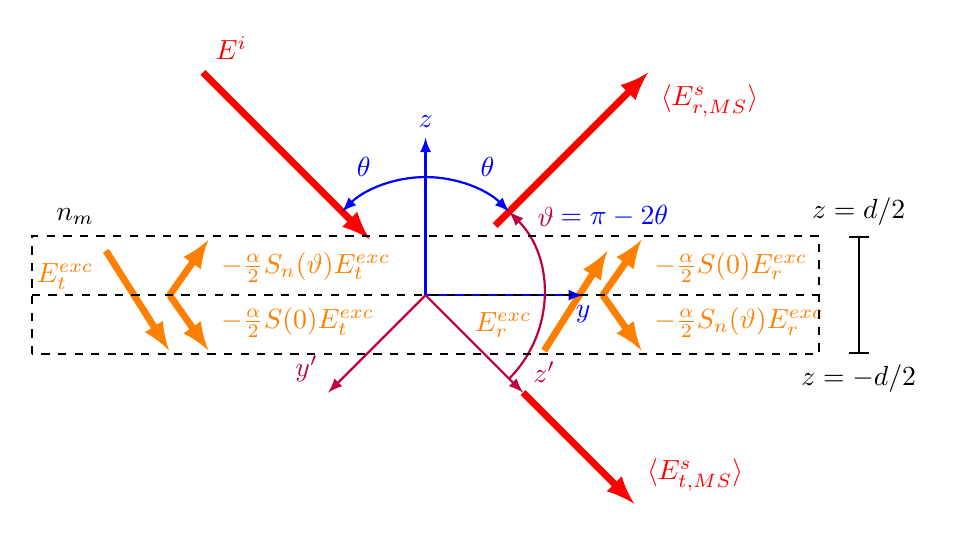
\begin{tikzpicture}[scale=1]
\def\a{.15}
\def\d{.75}

%\foreach \y in {-4.5,-3.5,-2.5,-.5,.5,2.5,3.5,4.5}{
%\fill[ball color=yellow, opacity=1] (\y+rand*.5,rand*\d) circle(\a) node[ ]{.};
%}


\draw[latex -, thick, red, line width=2.5](135:1)--(135:4) node[anchor=south west]{$\vb{E}^i$};
\draw[- latex, thick, red, line width=2.5](45:\d+.5)--(45:4)node[anchor=north west]{$\langle\vb{E}_{r,MS}^s\rangle$};
\draw[ - latex, thick, red, line width=2.5](-45:1.75)--(-45:3.75) node[anchor=south west]{$\langle\vb{E}_{t,MS}^s\rangle$};

%---------------------- Exciting transmitted field ---------------------
\draw[latex - , thick,  orange, line width=2.5,shift={(-3., 0)}](250:\d)--(152:1.2) node[anchor= north east]{$\vb{E}^{exc}_t$};

\draw[- latex , thick,  orange, line width=2.5, shift={(-2.5, 0)}](180:\d)--(250:\d) node[anchor= south west]{$-\frac{\alpha}{2} S(0)\vb{E}^{exc}_t$};
\draw[- latex , thick,  orange, line width=2.5, shift={(-2.5, 0)}](180:\d)--(110:\d) node[anchor= north west]{$-\frac{\alpha}{2} S_n(\vartheta)\vb{E}^{exc}_t$};

%---------------------- Exciting reflected field ---------------------
\draw[ latex -, thick, orange, line width=2.5,shift={(1.25, 0)}](28:1.2)--(-70:\d) node[anchor= south east]{$\vb{E}^{exc}_r$};

\draw[- latex , thick,  orange, line width=2.5, shift={(3., 0)}](180:\d)--(250:\d) node[anchor= south west]{$-\frac{\alpha}{2} S_n(\vartheta)\vb{E}^{exc}_r$};
\draw[- latex , thick,  orange, line width=2.5, shift={(3., 0)}](180:\d)--(110:\d) node[anchor= north west]{$-\frac{\alpha}{2}S(0)\vb{E}^{exc}_r$};

%----------------------Main system---------------------
\draw[- latex, thick, blue] (0,0)--(90:2) node[anchor = south]{$z$};
\draw[- latex, thick, blue] (0,0)--(0:2) node[anchor = north]{$y$};
\path (0,0)++(135/2:1.5)node[anchor=south west, blue]{$\theta$}; 
\draw[- latex, thick, blue](90:1.5)arc(90:45:1.5);
\path (0,0)++(90+45/2:1.5)node[anchor=south east, blue]{$\theta$}; 
\draw[- latex, thick, blue](90:1.5)arc(90:135:1.5);

%----------------------Mie system---------------------
\draw[- latex, thick, purple] (0,0)--(-45:1.75) node[anchor =south west]{$z'$};
\draw[- latex, thick, purple] (0,0)--(-135:1.75) node[anchor =south east]{$y'$};
\path (0,0)++(30:1.5)node[anchor=south west, purple]{$\vartheta$}; 
\path (0,0)++(30:1.5)node[anchor=south west, blue]{$\;\;\; =  \pi - 2\theta$}; 
\draw[- latex, thick, purple](-45:1.5)arc(-45:45:1.5);

%----------------------thickness and slab ---------------------
\draw[thick, dashed] (-5,-\d) rectangle (5,\d);
\draw[thick, dashed] (-5, 0) --  (5,0);
\draw[ |-|, thick,] (5.5,-\d) node[anchor = north]{$z=-d/2$} -- (5.5,\d) node[anchor = south]{$z=d/2$};
\node at (-4.5,1) {$\; n_m$};

\end{tikzpicture}
	\caption{  Película de grosor $d\to 0$ con y volumen $V$ con $N$ partículas esféricas idénticas y una onda incidente en la dirección $\vb{k}^i$. La dirección de los campos esparcidos coeherentes están dadas por $\vb{k}^r_{coh}$ y $\vb{k}^t_{coh}$. Las flechas rojas sólidas representan las componentes coehrentes del campo esparcido mientras que las rosas represetan su componente difusa. }\label{fig:Eexc}
	\end{figure}	
	

Al resolver para $E^{exc}_t$ y $E^{exc}_r$ se obtienen las expresiones
	\begin{align}
	\vb{E}^{exc}_t  &= \frac{\qty[1+\frac12\alpha S(0)]}
				{1+\alpha S(0) +\frac14\alpha^2\qty[S^2(0)-S_n^2(\vartheta)]}\vb{E}_0,\\
	\vb{E}^{exc}_r  &= \frac{-\frac12\alpha S_n(\vartheta)}
				{1+\alpha S(0) +\frac14\alpha^2\qty[S^2(0)-S_n^2(\vartheta)]}\vb{E}_0.
	\end{align}
por lo que, al sustituilas en las expresiones de los campos esparcidos promedio reflejados y transmitidos [Ecs. \eqref{eq:EsMS}] se obtienen
	\begin{align*}
	\langle \vb{E}^s_{r,coh}\rangle &=
			\frac{-\alpha S_n(\vartheta)}{1+\alpha S(0)+\frac14 \alpha^2 \left[S^2(0)-S_n^2 (\vartheta) \right]} \vb{E}_0 e^{i\vb{k}^r_{coh}\cdot\vb{r}},\\
	\langle \vb{E}^s_{r,coh}\rangle &=
			\frac{1-\frac14\alpha^2\qty[S^2(0)-S_n^2(\vartheta)]}{1+\alpha S(0)+\frac14 \alpha^2 \left[S^2(0)-S_n^2 (\vartheta) \right]} \vb{E}_0 e^{i\vb{k}^t_{coh}\cdot\vb{r}},
	\end{align*}
de donde es posible calcular los coeficientes de amplitud del CSM al considerar que $\vartheta = \pi-2\theta$, que el campo eléctrico que excita a las NPs toma en cuenta el esparcimiento múltiple y que la componente coherente del campo esparcido es mucho mayor que la contribución de la componente difusa, dando como resultado \vspace*{-.75em}
	\begin{subequations}\begin{tcolorbox}[title = Coeficientes de amplitud del CSM, breakable ]
	\begin{align}
	r_{coh}&=\frac{-\alpha S_n(\pi-2\theta)}
				{1+\alpha S(0)+\frac14 \alpha^2 \left[S^2(0)-S_n^2 (\pi-2\theta) \right]},
			\label{eqs:rcoh}\\
	t_{coh}&=\frac{1-\frac14\alpha^2\qty[S^2(0)-S_n^2(\pi-2\theta)]}
				{1+\alpha S(0)+\frac14 \alpha^2 \left[S^2(0)-S_n^2 (\pi-2\theta) \right]}.
		\label{eqs:tcoh}
	\end{align}
	con $n=1$ para polarización $s$, $n=2$ para $p$ y $S(0)=S_1(0)=S_2(0)$.
	\end{tcolorbox}\label{eq:rtcoh}\end{subequations}\vspace*{-.75em}\noindent


	 \subsection{Monocapa sobre un sustrato}

Las Ecs. \eqref{eq:rtcoh} son los coeficientes de amplitud de reflexión y transmisión de una onda plana $\vb{E}^i$ que incide a un ángulo $\theta$ sobre una monocapa de NPs esféricas, idénticas, de radio $a$ e índice de refracción $n_p$ ordenadas de forma aleatoria e inmersa en una matriz con índice de refracción $n_m$. Sin embargo, de forma experimental las NPs no están en un espacio libre, sino que son soportadas por un sustrato, de índice de refracción $n_s$; adicionalmente la incidencia del haz de luz puede ser en configuración externa, como se muestra en la Fig. \ref{figs:CSM-Ext}, o en una configuración en ATR, como se muestra en la Fig. \ref{figs:CSM-ATR}.

	\begin{figure}[h!]\centering
	\begin{subfigure}{.05\textwidth}\vspace{-4.5cm}\caption{}\label{figs:CSM-Ext}\end{subfigure}\hspace*{-2em}
	\begin{subfigure}{.48\textwidth}
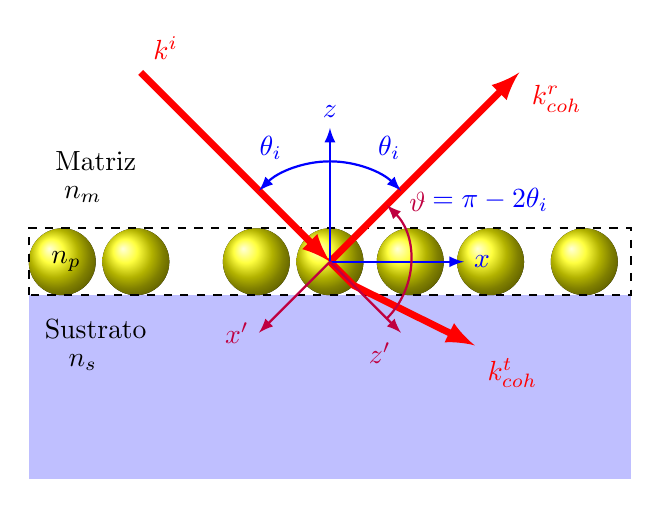
\begin{tikzpicture}[scale=.85]
\def\a{. 5}
\def\d{. 5}

\fill[blue, opacity=. 25] (-4. 5,-6.5*\d) rectangle (4. 5,-\d);

\foreach \x in {-4,-2. 9,-1. 1,0,1. 2,2. 4,3. 8}{
\fill[ball color=yellow, opacity=1] (\x,0) circle(\a);}


\draw[thick, dashed] (-4. 5,-\d) rectangle (4. 5,\d);

\draw[latex -, thick, red, line width=2. 5](135:0)--(135:4) node[anchor=south west]{$\vb{k}^i$};
\draw[- latex, thick, red, line width=2. 5](135:0)--(135:-.5)--(150:-2.5) node[anchor=north west]{$\vb{k}^t_{coh}$};
\draw[- latex, thick, red, line width=2. 5](45:0)--(45:4)node[anchor=north west]{$\vb{k}^r_{coh}$};

\draw[- latex, thick, blue] (0,0)--(90:2) node[anchor = south]{$z$};
\draw[- latex, thick, blue] (0,0)--(0:2) node[anchor = west]{$x$};
\path (0,0)++(135/2:1. 5)node[anchor=south west, blue]{$\theta_i$}; 
\draw[- latex, thick, blue](90:1. 5)arc(90:45:1. 5);
\path (0,0)++(90+45/2:1. 5)node[anchor=south east, blue]{$\theta_i$}; 
\draw[- latex, thick, blue](90:1. 5)arc(90:135:1. 5);

\draw[- latex, thick, purple] (0,0)--(-45:1. 5) node[anchor = north east]{$z'$};
\draw[- latex, thick, purple] (0,0)--(-135:1. 5) node[anchor = east]{$x'$};
\path (0,0)++(30:1. 2)node[anchor=south west, purple]{$\vartheta$}; 
\path (0,0)++(30:1. 2)node[anchor=south west, blue]{$\;\;\; =  \pi - 2\theta_i$}; 
\draw[- latex, thick, purple](-45:1. 2)arc(-45:45:1. 2);



\node at (-3.5,1.5) {Matriz};
\node at (-3.75,1) {$\; n_m$};
\node at (-4,0) {$\; n_p$};
\node at (-3.75,-1.5) {$\; n_s$};
\node at (-3.5,-1) {Sustrato};	
\end{tikzpicture}
	\end{subfigure}
	\begin{subfigure}{.05\textwidth}\vspace{-4.5cm}\caption{}\label{figs:CSM-ATR}	\end{subfigure}\hspace*{-2em}
	\begin{subfigure}{.48\textwidth} 
		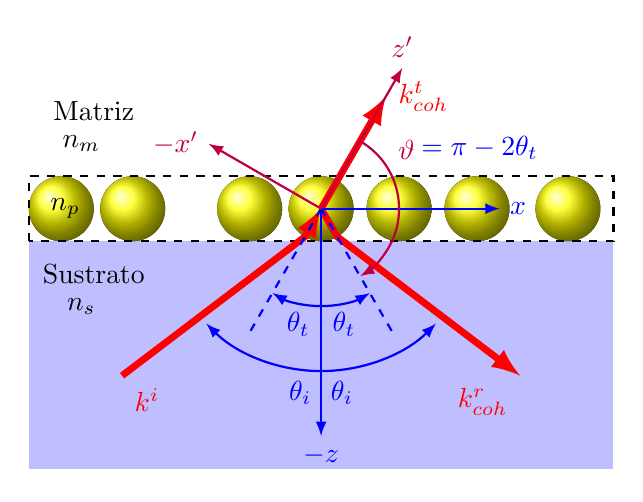
\begin{tikzpicture}[scale=.825]
\def\a{. 5}
\def\d{. 5}

\fill[blue, opacity=. 25] (-4. 5,-8*\d) rectangle (4. 5,-\d);

\foreach \x in {-4,-2. 9,-1. 1,0,1. 2,2. 4,3. 8}{
\fill[ball color=yellow, opacity=1] (\x,0) circle(\a);}


\draw[thick, dashed] (-4. 5,-\d) rectangle (4. 5,\d);

\draw[latex -, thick, red, line width=2. 5](0,0)--(-120:. 5)--(-140:4) node[anchor=north west]{$\vb{k}^i$};
\draw[- latex, thick, red, line width=2. 5](0,0)--(-120:-2)node[anchor=west]{$\vb{k}^t_{coh}$};
\draw[- latex, thick, red, line width=2. 5](0,0)--(-60:. 5)--(-40:4)node[anchor=north east]{$\vb{k}^r_{coh}$};

\draw[- latex, thick, blue] (0,0)--(-90:3. 5) node[anchor = north]{$-z$};
\draw[- latex, thick, blue] (0,0)--(0:2. 75) node[anchor = west]{$x$};

\path (0,0)++(-90:2. 5)node[anchor=north east, blue]{$\theta_i$}; 
\draw[- latex, thick, blue](-90:2. 5)arc(-90:-45:2. 5);
\path (0,0)++(-90:2. 5)node[anchor=north west, blue]{$\theta_i$}; 
\draw[- latex, thick, blue](-90:2. 5)arc(-90:-135:2. 5);

\draw[thick, blue, dashed](0,0) -- (-120:2. 25);
\draw[thick, blue, dashed](0,0) -- (-60:2. 25);
\path (0,0)++(-90-50/2:1. 6)node[anchor=north west, blue]{$\theta_t$}; 
\draw[- latex, thick, blue](-90:1. 5)arc(-90:-60:1. 5);
\path (0,0)++(-90+50/2:1. 6)node[anchor=north east, blue]{$\theta_t$}; 
\draw[- latex, thick, blue](-90:1. 5)arc(-90:-120:1. 5);

\draw[- latex, thick, purple] (0,0)--(60:2.5) node[anchor = south]{$z'$};
\draw[- latex, thick, purple] (0,0)--(150:2) node[anchor =  east]{$-x'$};
\path (0,0)++(30:1. 2)node[anchor=south west, purple]{$\vartheta$}; 
\path (0,0)++(30:1. 2)node[anchor=south west, blue]{$\;\;\; =  \pi - 2\theta_t$}; 
\draw[- latex, thick, purple](60:1. 2)arc(60:-60:1. 2);


\node at (-3.5,1.5) {Matriz};
\node at (-3.75,1) {$\; n_m$};
\node at (-4,0) {$\; n_p$};
\node at (-3.75,-1.5) {$\; n_s$};
\node at (-3.5,-1) {Sustrato};	
\end{tikzpicture}
	\end{subfigure}
	\caption{Esquema de la reflexión coeherente de una monocapa de NPs esféricas  suspendida en un a matriz con índice de refracción $n_m$ y soportada por un sustrato con índice de refracción $n_s$ en \textbf{a)} incidencia externa  y \textbf{b)} en configuración ATR.  EL sistema coordenado azul es colocado sobre la monocapa y con el eje $z$ normal a ésta; el sistema coordenado morado se alínea,  en su dirección $z$, con la dirección de propagación de la luz al incidir sobre la NP, por lo que es el sistema coordenado empleado en la solución de Mie. }	\label{fig:CSM-Diagrams}	
	\end{figure}	

En las Fig. \ref{fig:CSM-Diagrams}	 se observa que el ángulo $\theta$ a evaluar $r_{coh}$ y $t_{coh}$ en las Ecs. \eqref{eq:rtcoh} depende del medio por el que incide el campo eléctrico de la onda plana, con dirección $\vb{k}^i$. En incidencia externa, Fig. \ref{figs:CSM-Ext}, la onda plana incide sobre las NPs a n ángulo $\theta_i$ dado que no interactúa con la interfaz matriz-sustrato y no modifica su trayectoria. De forma contraria, en una configuración ATR, Fig. \ref{figs:CSM-ATR}, la onda plana cruza la interfaz sustrato-matriz, por lo que se refracta a un ángulo $\theta_t$ dado por la ley de Snell, e incide a la monocapa en $\theta=\theta_t$. Además de considerar el ángulo con el que la onda plana ilumina a las NPs, se debe calcular la contribución del sustrato en la reflectancia $R$ y transmitancia $T$ que también depende de medio por donde incida la onda plana.

Para calcular la refelctancia y transmitancia del sistema matriz-monocapa-sustrato, es decir, en incidencia externa, se consideran las múltiples reflexiones del sistema, mostradas en la Fig. \ref{fig:CSM-externa}. Cuando la onda plana con amplitud $E_i$ incide en la monocapa, en $z=2a$, se presenta una primera reflexión dada por el CSM, es decir que la amplitud del campo eléctrico en la primera reflexión es $r_{coh}E_i$. La segunda reflexión se presenta tras dos transmisiones en la monocapa y una reflexión en la interfaz matriz-sustrato, con una diferencia de fase $2\beta=2(2ak_m\cos\theta)$ respecto a la primera reflexión, es decir, que la amplitud de la segunda reflexión es $t_{coh}^2r_{ms}e^{i2\beta}E_i$. En la tercera reflexión hay dos transmisiones en la monocapa, dos reflexiones en la interfaz matriz-sustrato, y una reflexión en la monocapa, al considerar la diferencia de camino óptico con la primera relfexión, la amplitud de la tercera reflexión es $t_{coh}^2r_{coh}r_{ms}^2e^{i4\beta}E_i$. Al considerar el resto de las reflexiones, se obtiene que el coeficiente de amplitud de reflexión del sistema $r$ es
	\begin{align}
	r = r_{coh} +
		 t_{coh}^2r_{ms}e^{i2\beta}+
		 t_{coh}^2r_{coh}r_{ms}^2e^{i4\beta}+
		 t_{coh}^2r_{coh}^2r_{ms}^3e^{i6\beta}+
		 t_{coh}^2r_{coh}^3r_{ms}^4e^{i8\beta}+\ldots
%		 t_{coh}^2r_{coh}^4r_{ms}^5e^{i10\beta}+\ldots
	\label{eq:r_ext_span}
	\end{align}
Para el cálculo de la transmitancia del sistema $t$ se hace un procedimiento análogo al de $r$: la primera transmisión ocurre después de una transmisión en la monocapa y una en la interfaz matriz-sustrato y una diferencia de fase de $\beta$, por lo que la amplitud de la primera transmisión es $t_{coh}t_{ms}e^{i\beta}$. Para la $m$-ésima transmisión se presentan $m-1$ reflexiones con la monocapa y $m-1$ con el sustrato, además de una fase de $(2m-1)\beta$, es decir,
	\begin{align}
	t = t_{coh}t_{ms}e^{i\beta} +
		t_{coh}r_{ms}r_{coh}t_{ms}e^{i3\beta}+
		t_{coh}r_{ms}^2r_{coh}^2t_{ms}e^{i5\beta}+	
		t_{coh}r_{ms}^3r_{coh}^3t_{ms}e^{i7\beta}+ \ldots					
%		t_{coh}r_{ms}^4r_{coh}^4t_{ms}e^{i9\beta}+ \ldots				
%		t_{coh}r_{ms}^5r_{coh}^5t_{ms}e^{i11\beta}+\ldots
	\label{eq:t_ext_span}
	\end{align}

\begin{figure}[t!]\centering
	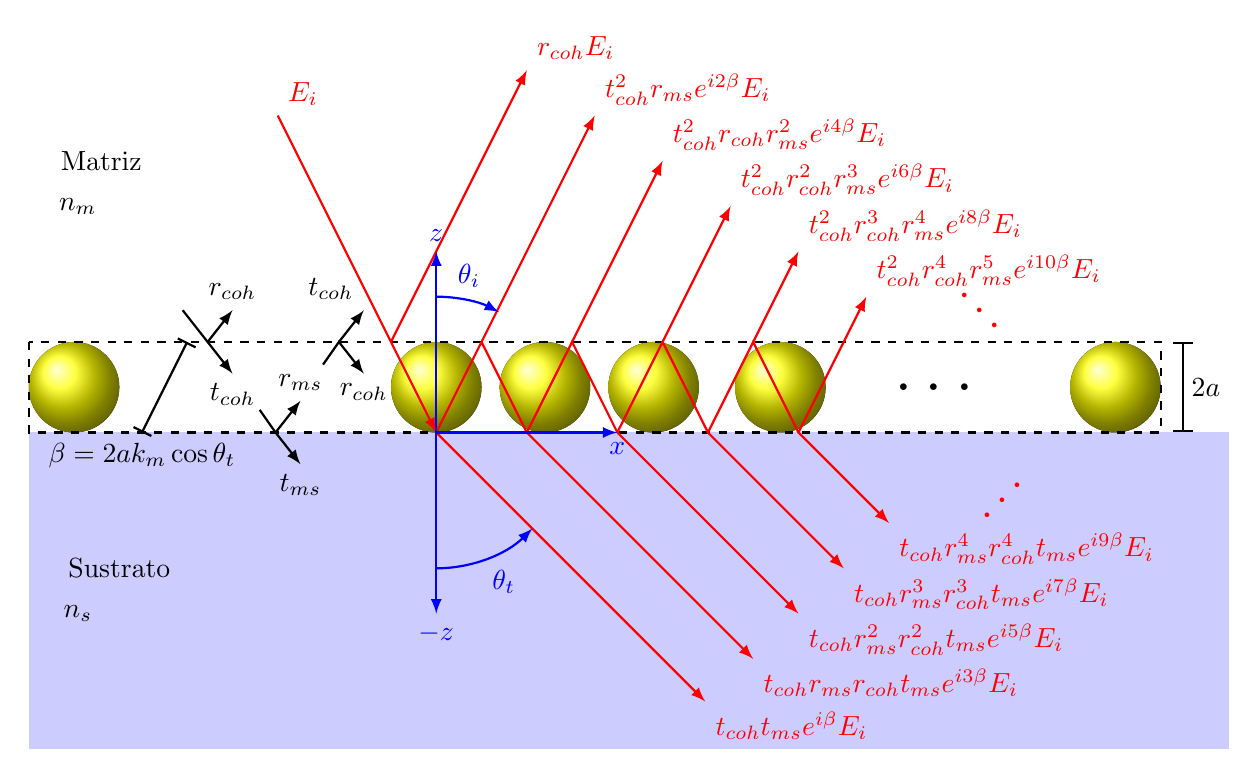
\begin{tikzpicture}[scale=1.15]
\def\a{.5}
\def\d{.5}
\def\t{.3}

\fill[blue, opacity = .2] (-4.5,-3.5) rectangle(8.75,0);

\foreach \x in {-4,0,1.2,2.4,3.8,7.5}{ %-2.9,-1.1
\fill[ball color=yellow, opacity=1] (\x,\d) circle(\a);}

\draw[thick, dashed] (-4.5,2*\d) rectangle (8,0);
\node at (5.5,\d) {\Huge $\ldots$};

%%%%%%%%%%%%%-------------transmisiones

\draw[- latex, thick, red](-135:0)--(-45:4.2) node[anchor=north west]{$t_{coh}t_{ms}e^{i\beta}E_i$};
\draw[- latex, thick, red](0,0)--(1*\d,2*\d)--(2*\d,0)--(3+\d,-3+\d) node[anchor=north west]{$t_{coh}r_{ms}r_{coh}t_{ms}e^{i3\beta}E_i$};
\draw[- latex, thick, red](2*\d,0)--(3*\d,2*\d)--(4*\d,0)--(3+2*\d,-3+2*\d) node[anchor=north west]{$t_{coh}r_{ms}^2r_{coh}^2t_{ms}e^{i5\beta}E_i$};
\draw[- latex, thick, red](4*\d,0)--(5*\d,2*\d)--(6*\d,0)--(3+3*\d,-3+3*\d) node[anchor=north west]{$t_{coh}r_{ms}^3r_{coh}^3t_{ms}e^{i7\beta}E_i$};
\draw[- latex, thick, red](6*\d,0)--(7*\d,2*\d)--(8*\d,0)--(3+4*\d,-3+4*\d) node[anchor=north west]{$t_{coh}r_{ms}^4r_{coh}^4t_{ms}e^{i9\beta}E_i$};
\draw[-, thick, red](8*\d,0)--(9*\d,2*\d);
\node[rotate={45}] at (6.25,-.75) {\color{red}\LARGE $\ldots$};


%%%%%%%%%%%%%-------------reflexiones
\draw[latex -, thick, red](0,0)--(-1.75,3.5) node[anchor=south west]{$E_i$};
\draw[- latex, thick, red](-1*\d,2*\d)--(2-2*\d,4+0*\d) node[anchor=south west]{$r_{coh}E_i$};
\draw[- latex, thick, red](1*\d,2*\d)--(1.75,3.5) node[anchor=south west]{$t_{coh}^2r_{ms}e^{i2\beta}E_i$};
\draw[- latex, thick, red](3*\d,2*\d)--(2+1*\d,4-2*\d) node[anchor=south west]{$ t_{coh}^2r_{coh}r_{ms}^2e^{i4\beta}E_i$};
\draw[- latex, thick, red](5*\d,2*\d)--(2+2.5*\d,4-3*\d) node[anchor=south west]{$ t_{coh}^2r_{coh}^2r_{ms}^3e^{i6\beta}E_i$};
\draw[- latex, thick, red](7*\d,2*\d)--(2+4*\d,4-4*\d) node[anchor=south west]{$ t_{coh}^2r_{coh}^3r_{ms}^4e^{i8\beta}E_i$};
\draw[- latex, thick, red](9*\d,2*\d)--(2+5.5*\d,4-5*\d) node[anchor=south west]{$t_{coh}^2r_{coh}^4r_{ms}^5e^{i10\beta}E_i$};
\node[rotate={-45}] at (6,1.35) {\color{red}\LARGE $\ldots$};



\node at (-4,2.5) {$\; n_m$};
\node at (-3.7,3) {Matriz};
\node at (-4,-2) {$\; n_s$};
\node at (-3.5,-1.5) {Sustrato};

%.55,0
%2,0
%1.2,2*\ḑ
%%\draw[latex - , thick](-2.8,-.5)--(-3.5,.5) node[anchor=north]{$r_{sm},\,t_{sm}$};
\draw[latex - , thick, shift ={(2,2*\d)}](-2.8,-.35)node[anchor=north]{$r_{coh}$}--(-3.075,0)--(-3.25,-.25);
\draw[latex -,thick, shift ={(2,2*\d)}](-2.8,.35)node[anchor=south east]{$t_{coh}$}--(-3.075,0);
\draw[latex - , thick, shift ={(.55,2*\d)}](-2.8,-.35)node[anchor=north]{$t_{coh}$}--(-3.075,0)--(-3.35,.35);
\draw[latex -,thick, shift ={(.55,2*\d)}](-2.8,.35)node[anchor=south]{$r_{coh}$}--(-3.075,0);
\draw[latex - , thick, shift ={(1.3,0)}](-2.8,-.35)node[anchor=north]{$t_{ms}$}--(-3.075,0)--(-3.25,+.25);
\draw[latex -,thick, shift ={(1.3,0)}](-2.8,.35)node[anchor=south]{$r_{ms}$}--(-3.075,0);

\draw[|-|,thick, shift ={(-3.25,0)}](0,0)node[anchor=north]{$\beta = 2ak_m\cos\theta_t$}--(1*\d,2*\d) ;

\draw[|-|,thick, shift ={(8.25,0)}](0,0)--(0,2*\d) ;
\node at (8.5,\d){$2a$};

\draw[- latex, thick, blue] (0,0)--(90:2) node[anchor = south]{$z$};
\draw[- latex, thick, blue] (0,0)--(90:-2) node[anchor = north]{$-z$};
\draw[- latex, thick, blue] (0,0)--(0:2) node[anchor = north]{$x$};
\path (0,0)++(85:1.5)node[anchor=south west, blue]{$\theta_i$}; 
\draw[- latex, thick, blue](90:1.5)arc(90:62.5:1.5);
\path (0,0)++(-70:1.5)node[anchor=north west, blue]{$\theta_t$}; 
\draw[- latex, thick, blue](-90:1.5)arc(-90:-45:1.5);


\end{tikzpicture}
	\caption{ Esquema de las múltiples reflexiones en incidencia externa del sistema matriz-monocapa-sustrato producidos por una onda plana $\vb{E}^i$ que incide en la interfaz de un sustrato, con índice de refracción $n_s$, que sostiene a una monocapa de NPs esféricas de radio $a$ inmerza en una matriz con $n_m$, a un ángulo $\theta_i$ respecto a la dirección normal a la interfaz. Las reflexiones y transmisionees en la interfaz sustrato-matriz ($z=0$) es descrita por los coeficientes de amplitud de Fresnel [Ecs. \eqref{eq:rs}--\eqref{eq:tp}], mientras que en la intfaz monocapa-matriz ($z=2a$) las reflexiones y transmisiones son descritsd por el CSM [Ecs. \eqref{eq:rtcoh}]. Los coeficientes de amplitud son evaluados en $\theta_i$ en $z=2a$. En los coeficientes de amplitud  $r_{\alpha\beta}$ y $t_{\alpha\beta}$ el medio de incidencia del haz de luz es $\alpha$ y el de transmisión en $\beta$.}\label{fig:CSM-externa}
	\end{figure}

Al factorizar $r_{ms}t_{coh}^2e^{2i\beta}$ en la Ec. \eqref{eq:r_ext_span}, a excepción del primer término $r_{coh}$, y factorizar $t_{coh}t_{ms}e^{i\beta}$ en la Ec. \eqref{eq:t_ext_span} se obtienen las expresiones
	\begin{align*}
	r &= r_{coh} + r_{ms}t_{coh}^2e^{2i\beta}\left[1+r_{coh}r_{ms}e^{2i\beta}+\qty(r_{coh}r_{ms}e^{2i\beta})^2+\qty(r_{coh}r_{ms}e^{2i\beta})^3+\ldots,\right.\\
	t &= t_{coh}t_{ms}e^{i\beta} \left[1+r_{coh}r_{ms}e^{2i\beta}+\qty(r_{coh}r_{ms}e^{2i\beta})^2+\qty(r_{coh}r_{ms}e^{2i\beta})^3+\ldots\right. ,
	\end{align*}
y dado que $\norm{r_{coh}r_{ms}e^{2i\beta}}<1$, es posible reescribir los coeficientes de amplitud del sistema como \vspace*{-.75em}\begin{subequations}
	\begin{tcolorbox}[title = Coeficientes de amplitud de CSM en incidencia externa, breakable ]
	\eqhalf{r = r_{coh}(\theta_i)+ \frac{r_{ms}(\theta_i)t_{coh}(\theta_i)e^{i2\beta}}
										{1-r_{coh}(\theta_i)r_{ms}(\theta_i)e^{2i\beta}},
	\label{eqs:rCSMext}}
	\eqhalf{t = \frac{t_{ms}(\theta_i)t_{coh}(\theta_i)e^{i\beta}}
									{1-r_{coh}(\theta_i)r_{ms}(\theta_i)e^{2i\beta}},
	\label{eqs:tCSMext}}
	
	con $\beta = 2a k_0n_m\cos\theta_i$.
	\end{tcolorbox}\label{eq:rtCSMext}\end{subequations}\vspace*{-.75em}

Cuando se considera que el haz de luz incide sobre el sistema con un ángulo $\theta_i$ en una confiuración  ATR, el haz de luz se refleja por la interfaz sustrato-matriz ($z=0$) a un ángulo  $\theta_i$ pero se transmite a un ángulo  $\theta_t$. El haz de luz ilumina a las NPs al ángulo $\theta_t$, y a este mismo ángulo se refleja y transmite a través de la monocapa (en $z=2a$), como se observa e la Fig. \ref{fig:CSM-ATR}, donde, por claridad, los subíndices $sm$ corresponden a los coeficientes de Fresnel evaluados en $\theta_i$; mientras que $ms$ y $coh$, en $\theta_t$. De forma análoga al caso de incidencia externa, el coeficiente de amplitud de reflexión y transmisión del sistema son
	\begin{align}
	r &= r_{sm}+ 
		t_{sm}r_{coh}r_{ms}e^{i2\beta}+
		t_{sm}r_{coh}^2r_{ms}e^{i4\beta}+
		t_{sm}r_{coh}^3r_{ms}^2e^{i6\beta}+
		t_{sm}r_{coh}^4r_{ms}^3e^{i8\beta}\ldots,
	\label{eq:r_ATR_span}\\		
	t &= t_{sm}t_{coh}e^{i\beta}+ 
		t_{sm}r_{coh}r_{ms}t_{coh}e^{i3\beta}+
		t_{sm}r_{coh}^2r_{ms}^2t_{coh}e^{i5\beta}+
		t_{sm}r_{coh}^3r_{ms}^3t_{coh}e^{i7\beta}+\ldots,	
%		t_{sm}r_{coh}^4r_{ms}^4t_{coh}e^{i9\beta}+\ldots,	
	\label{eq:t_ATR_span}
	\end{align}
donde $\beta = 2ak_m\cos\theta_t$. Al factorizar $t_{sm}r_{coh}t_{ms}e^{2i\beta}$ en la Ec. \eqref{eq:r_ATR_span} y $t_{sm}t_{coh}e^{i\beta}$ en la Ec. \eqref{eq:t_ATR_span}, y considerar que $\norm{r_{coh}r_{ms}e^{i2\beta}}<1$, los coeficientes de amplitud son


\begin{figure}[t!]\centering
	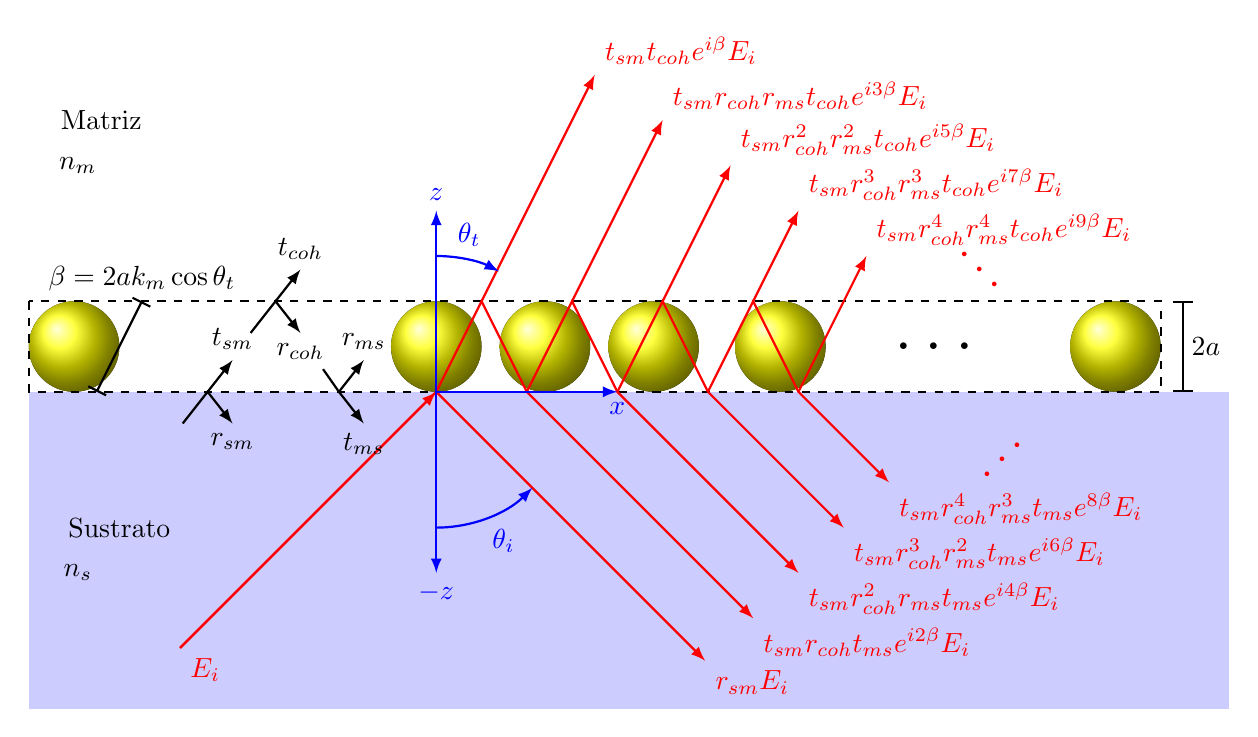
\begin{tikzpicture}[scale=1.15]
\def\a{.5}
\def\d{.5}
\def\t{.3}

\fill[blue, opacity = .2] (-4.5,-3.5) rectangle(8.75,0);

\foreach \x in {-4,0,1.2,2.4,3.8,7.5}{ %-2.9,-1.1
\fill[ball color=yellow, opacity=1] (\x,\d) circle(\a);}

\draw[thick, dashed] (-4.5,2*\d) rectangle (8,0);
\node at (5.5,\d) {\Huge $\ldots$};


%%%%%%%%%%%%%-------------Reflexiones
%
%\draw[latex -, thick, red](-135:0)--(-135:4) node[anchor=north]{$E_i$};
%\draw[- latex, thick, red](-135:4)--(-135:0)--(-45:4) node[anchor=north]{$r_{coh}E_i$};
%\draw[- latex, thick, red](0,0)--(2*\d,2*\d)--(3+2*\d,-3+2*\d) node[anchor=south west]{$t_{coh}r_{ms}t_{coh}E_i$};
%\draw[- latex, thick, red](4*\d,0)--(6*\d,2*\d)--(3+6*\d,-3+2*\d) node[anchor=south west]{$r_{coh}E_i$};


\draw[latex -, thick, red](-135:0)--(-135:4) node[anchor=north west]{$E_i$};
\draw[- latex, thick, red](-135:4)--(-135:0)--(-45:4.2) node[anchor=north west]{$r_{sm}E_i$};
\draw[- latex, thick, red](0,0)--(1*\d,2*\d)--(2*\d,0)--(3+\d,-3+\d) node[anchor=north west]{$t_{sm}r_{coh}t_{ms}e^{i2\beta}E_i$};
\draw[- latex, thick, red](2*\d,0)--(3*\d,2*\d)--(4*\d,0)--(3+2*\d,-3+2*\d) node[anchor=north west]{$t_{sm}r_{coh}^2r_{ms}t_{ms}e^{i4\beta}E_i$};
\draw[- latex, thick, red](4*\d,0)--(5*\d,2*\d)--(6*\d,0)--(3+3*\d,-3+3*\d) node[anchor=north west]{$t_{sm}r_{coh}^3r_{ms}^2t_{ms}e^{i6\beta}E_i$};
\draw[- latex, thick, red](6*\d,0)--(7*\d,2*\d)--(8*\d,0)--(3+4*\d,-3+4*\d) node[anchor=north west]{$t_{sm}r_{coh}^4r_{ms}^3t_{ms}e^{8\beta}E_i$};
\draw[-, thick, red](8*\d,0)--(9*\d,2*\d);
\node[rotate={45}] at (6.25,-.75) {\color{red}\LARGE $\ldots$};

%%%%%%%%%%%%%-------------transmisiones
\draw[- latex, thick, red](1*\d,2*\d)--(1.75,3.5) node[anchor=south west]{$t_{sm}t_{coh}e^{i\beta}E_i$};
\draw[- latex, thick, red](3*\d,2*\d)--(2+1*\d,4-2*\d) node[anchor=south west]{$t_{sm}r_{coh}r_{ms}t_{coh}e^{i3\beta}E_i$};
\draw[- latex, thick, red](5*\d,2*\d)--(2+2.5*\d,4-3*\d) node[anchor=south west]{$t_{sm}r_{coh}^2r_{ms}^2t_{coh}e^{i5\beta}E_i$};
\draw[- latex, thick, red](7*\d,2*\d)--(2+4*\d,4-4*\d) node[anchor=south west]{$t_{sm}r_{coh}^3r_{ms}^3t_{coh}e^{i7\beta}E_i$};
\draw[- latex, thick, red](9*\d,2*\d)--(2+5.5*\d,4-5*\d) node[anchor=south west]{$t_{sm}r_{coh}^4r_{ms}^4t_{coh}e^{i9\beta}E_i$};
\node[rotate={-45}] at (6,1.35) {\color{red}\LARGE $\ldots$};



\node at (-4,2.5) {$\; n_m$};
\node at (-3.7,3) {Matriz};
\node at (-4,-2) {$\; n_s$};
\node at (-3.5,-1.5) {Sustrato};

%\draw[latex - , thick](-2.8,-.5)--(-3.5,.5) node[anchor=north]{$r_{sm},\,t_{sm}$};
\draw[latex - , thick, shift ={(.55,0)}](-2.8,-.35)node[anchor=north]{$r_{sm}$}--(-3.075,0)--(-3.35,-.35);
\draw[latex -,thick, shift ={(.55,0)}](-2.8,.35)node[anchor=south]{$t_{sm}$}--(-3.075,0);
\draw[latex - , thick, shift ={(2.0,0)}](-2.8,-.35)node[anchor=north]{$t_{ms}$}--(-3.075,0)--(-3.25,.25);
\draw[latex -,thick, shift ={(2.0,0)}](-2.8,.35)node[anchor=south]{$r_{ms}$}--(-3.075,0);
\draw[latex - , thick, shift ={(1.3,2*\d)}](-2.8,-.35)node[anchor=north]{$r_{coh}$}--(-3.075,0)--(-3.35,-.35);
\draw[latex -,thick, shift ={(1.3,2*\d)}](-2.8,.35)node[anchor=south]{$t_{coh}$}--(-3.075,0);

\draw[|-|,thick, shift ={(-3.75,0)}](0,0)--(1*\d,2*\d) node[anchor=south]{$\beta = 2ak_m\cos\theta_t$};

\draw[|-|,thick, shift ={(8.25,0)}](0,0)--(0,2*\d) ;
\node at (8.5,\d){$2a$};

\draw[- latex, thick, blue] (0,0)--(90:2) node[anchor = south]{$z$};
\draw[- latex, thick, blue] (0,0)--(90:-2) node[anchor = north]{$-z$};
\draw[- latex, thick, blue] (0,0)--(0:2) node[anchor = north]{$x$};
\path (0,0)++(85:1.5)node[anchor=south west, blue]{$\theta_t$}; 
\draw[- latex, thick, blue](90:1.5)arc(90:62.5:1.5);
\path (0,0)++(-70:1.5)node[anchor=north west, blue]{$\theta_i$}; 
\draw[- latex, thick, blue](-90:1.5)arc(-90:-45:1.5);


\end{tikzpicture}
	\caption{ Esquema de las múltiples reflexiones en ATR del sistema matriz-monocapa-sustrato producidos por una onda plana $\vb{E}^i$ que incide en la interfaz de un sustrato, con índice de refracción $n_s$, que sostiene a una monocapa de NPs esféricas de radio $a$ inmerza en una matriz con $n_m$, a un ángulo $\theta_i$ respecto a la dirección normal a la interfaz. Las reflexiones y transmisionees en la interfaz sustrato-matriz ($z=0$) es descrita por los coeficientes de amplitud de Fresnel [Ecs. \eqref{eq:rs}--\eqref{eq:tp}] en $\theta_i$, mientras que en la intfaz monocapa-matriz ($z=2a$) las reflexiones y transmisiones son descritsd por el CSM [Ecs. \eqref{eq:rtcoh}] en $\theta_t$. En los coeficientes de amplitud  $r_{\alpha\beta}$ y $t_{\alpha\beta}$ el medio de incidencia del haz de luz es $\alpha$ y el de transmisión en $\beta$.}\label{fig:CSM-ATR}
	\end{figure}

	\begin{align}
	r =& r_{sm} + t_{sm}r_{coh}t_{ms}e^{2i\beta}\left[1+r_{coh}r_{ms}e^{2i\beta}+\qty(r_{coh}r_{ms}e^{2i\beta})^2+\qty(r_{coh}r_{ms}e^{2i\beta})^3+\ldots,\right. \notag \\
		=& r_{sm} + \frac{ t_{sm}r_{coh}t_{ms}e^{2i\beta}}
				{1-r_{ms}r_{coh}e^{i2\beta}}, \label{eq:r_ATR_preStokes} \\
	t =& t_{coh}t_{ms}e^{i\beta} \left[1+r_{coh}r_{ms}e^{2i\beta}+\qty(r_{coh}r_{ms}e^{2i\beta})^2+\qty(r_{coh}r_{ms}e^{2i\beta})^3+\ldots\right. 
	=\frac{  t_{coh}t_{ms}e^{i\beta} }
				{1-r_{ms}r_{coh}e^{i2\beta}}.\notag
	\end{align}
Es posible reescribir la Ec. \ref{eq:r_ATR_preStokes} empleando las relaciones de Stokes\footnote{Las relaciones de Stokes se deducar a partir de lainvariancia de las ecuaciones de Maxell ante inversiones temporales ($t\to -t$), y relacionan a los coeficientes de amplitud $r$ y $t$ evaluados en $\theta_i$ y $\theta_t$ para una interfaz entre medios no absorbentes. Las relaciones de Stokes son \cite{hecht1998optics,garcia2012multiple} $r_{it}(\theta_i) = -r_{ti}(\theta_t)$, $t_{it}(\theta_i) = 1+r_{it}(\theta_i)$, y $t_{ti}(\theta_t) = 1+r_{it}(\theta_t)$}, por lo que se obtiene \begin{subequations}\vspace*{-.75em}
\begin{tcolorbox}[title = Coeficientes de amplitud de CSM en configuración ATR, breakable ]
	\eqhalf{t = \frac{r_{sm}(\theta_i)+r_{coh}(\theta_t)e^{i2\beta}}
					{1+-r_{coh}(\theta_t)r_{sm}(\theta_i)e^{2i\beta}},
	\label{eqs:rCSMATR}}
	\eqhalf{t = \frac{t_{sm}(\theta_i)t_{coh}(\theta_t)e^{i\beta}}
									{1-r_{coh}(\theta_t)r_{ms}(\theta_t)e^{2i\beta}},
	\label{eqs:tCSMATR}}
	
	con $\beta = 2a k_0n_m\cos\theta_t$.
	\end{tcolorbox}\label{eq:rtCSMext}\end{subequations}\vspace*{-.75em}












